\chapter{Phase II upgrade of the CMS Tracker}  %Title of the First Chapter

\ifpdf
    \graphicspath{{Chapter7/Figs/Raster/}{Chapter7/Figs/PDF/}{Chapter7/Figs/}}
\else
    \graphicspath{{Chapter7/Figs/Vector/}{Chapter7/Figs/}}
\fi

%\section{Overview of the Phase II upgrade of the CMS Tracker}
%\label{sec:PhaseIItracker}

The Phase II upgrade of the CMS Tracker is a crucial project undertaken to maintain the effectiveness of the CMS experiment during the High Luminosity LHC (HL-LHC) run, which is expected to start in 2027. The HL-LHC will significantly increase the instantaneous luminosity, leading to a higher number of proton-proton collisions per bunch crossing. This higher collision rate poses several challenges, including increased radiation levels, higher data rates, and more complex event environments. The Phase II upgrade of the CMS tracker comprises two main components: the Inner Tracker (IT) and the Outer Tracker (OT). The Inner Tracker consists of three main sub-components: the TEPX (Tracker Endcap Pixel), the TFPX (Tracker Forward Pixel), and the TBPX (Tracker Barrel Pixel) detectors. These sub-components are designed to handle the increased radiation levels and data rates in the HL-LHC environment. The Outer Tracker is responsible for detecting charged particles in the outer region of the CMS detector. It consists of two key subsystems: the silicon strip tracker and the silicon macro pixel tracker.

%The Phase II upgrade of the CMS tracker is a major upgrade of the tracking system of the Compact Muon Solenoid (CMS) experiment at the Large Hadron Collider (LHC) at CERN. The upgrade is designed to improve the performance of the CMS tracker, enabling more precise measurements of the properties of particles produced in proton-proton collisions at the LHC.

\begin{enumerate}

\item Inner Tracker: The Inner Tracker is the innermost part of the CMS Tracker, closest to the collision point. It is designed to provide high-resolution position measurements of charged particles in a high-density environment, as well as excellent radiation tolerance. The Inner Tracker is crucial for the precise determination of the primary and secondary vertices (interaction points) and the accurate reconstruction of decay paths of short-lived particles. The Inner Tracker of the CMS experiment during the Phase II Upgrade will consist of three main subcomponents: TEPX (Tracker Endcap Pixel), TFPX (Tracker Forward Pixel), and TBPX (Tracker Barrel Pixel). These subsystems together form the new high-resolution, highly granular, and radiation-tolerant pixel tracking system.

\begin{itemize}

\item TBPX (Tracker Barrel Pixel): The TBPX subsystem is located in the central region of the Inner Tracker, arranged in a barrel geometry around the beam axis. It consists of several concentric cylindrical layers of high-resolution pixel sensors, providing precise measurements of charged particle trajectories in the xy-plane. The upgraded TBPX will feature higher granularity pixel sensors to better handle the increased event rates and radiation levels expected during the HL-LHC era.

\item TFPX (Tracker Forward Pixel): The TFPX subsystem covers the forward regions of the Inner Tracker, extending the coverage in the pseudorapidity ($\eta$) direction. Like the TBPX, it consists of high-resolution pixel sensors, arranged in multiple concentric discs around the beam axis. The TFPX will provide precise position measurements for charged particles in the forward and backward regions, complementing the coverage provided by the TBPX.

\item TEPX (Tracker Endcap Pixel): The TEPX subsystem is located further out in the forward and backward regions, surrounding the TFPX subsystem. It consists of additional concentric discs of pixel sensors, further extending the tracking coverage in the pseudorapidity direction. The TEPX helps to ensure efficient tracking performance in the high-$\eta$ regions, where the particle density is lower compared to the central region.

\end{itemize}

%The TBPX, TFPX, and TEPX subsystems will form a highly efficient, high-resolution Inner Tracker capable of providing precise position measurements for charged particles produced in proton-proton collisions at the LHC. The upgraded pixel-based Inner Tracker will be crucial for maintaining the CMS experiment's excellent performance during the high-luminosity and high-radiation environment expected during the HL-LHC era.

\item Outer Tracker: The Outer Tracker is designed to provide additional tracking points for charged particles as they traverse through the CMS detector. This extra information helps improve the overall track reconstruction accuracy and efficiency. In the Phase II Upgrade, the Outer Tracker will be based on the novel concept of "Tracker-Trigger," which combines tracking and triggering functionalities.

\begin{itemize}

\item In the upgraded Outer Tracker, silicon strip sensors will be used to form "trigger primitives" - early-stage track candidates - that are passed to the Level-1 Trigger system. This approach helps to reduce the data volume and allows the CMS experiment to maintain its excellent physics performance in the face of increased event rates.

\item The Outer Tracker will consist of multiple layers of strip sensor modules, organized in barrel and endcap regions. The sensor modules will be connected to custom-designed readout electronics that process the data in real-time and transmit the trigger primitives to the Level-1 Trigger system.

\end{itemize}

%\end{enumerate}

%\item Pixel Detector: The new pixel detector will have smaller pixels than the existing one, which will improve the spatial resolution of the detector. The new pixels will be 50 x 50 micrometers in size, compared to 100 x 150 micrometers in the existing detector. The new detector will also be more radiation tolerant, which means that it will be able to withstand the high radiation levels near the LHC beamline without losing performance. The new detector will consist of four barrel layers and six forward disks, providing coverage out to a pseudorapidity of 4.

%\begin{enumerate}
%\renewcommand{\labelenumi}{\roman{enumi})}
 %\item Tracker Endcap Pixel detector (TEPX): TEPX is a specialized pixel detector that will be added to the endcap region of the CMS tracker. It will be located in the forward region of the detector, covering a pseudorapidity range of 1.8 to 2.9. TEPX will consist of two disks on each side of the detector, with each disk containing 96 modules of pixel sensors.

%\item Tracker Forward Pixel detector (TFPX): TFPX is a specialized pixel detector that will be added to the forward region of the CMS tracker. It will be located in front of the existing pixel detector and will cover a pseudorapidity range of 2.5 to 4.0. TFPX will consist of four disks on each side of the detector, with each disk containing 24 modules of pixel sensors.

%\item Tracker Barrel Pixel detector (TBPX): TBPIX is a specialized pixel detector that will be added to the barrel region of the CMS tracker. It will be located in between the existing pixel detector layers and will cover a pseudorapidity range of 0 to 2.5. TBPIX will consist of four layers of pixel sensors, each layer containing 192 modules.

%\end{enumerate}

%\item Strip Detector: The new strip detector will have larger and thinner silicon sensors, which will improve the spatial resolution of the detector. The new sensors will be 100 micrometers thick, compared to 320 micrometers in the existing detector, and they will be up to 12 centimeters long, compared to 10 centimeters in the existing detector. The new readout electronics will be faster and more radiation tolerant than the existing ones. The new strip detector will have a total of 10 layers, providing coverage out to a pseudorapidity of 2.7.

\item Timing layer is a new addition to the CMS Tracker during the Phase II upgrade, designed to provide precise time measurements of charged particles passing through the detector. These measurements help in distinguishing between particles originating from different vertices in the same event and reducing the impact of pileup on event reconstruction. The timing layer uses Low Gain Avalanche Detectors (LGAD) as the active material. LGADs are a type of silicon sensor that incorporates a multiplication layer to generate an avalanche of charge carriers when a charged particle passes through the detector. This multiplication process results in a faster signal response and improved time resolution compared to traditional silicon sensors. When a charged particle traverses the timing layer, it creates electron-hole pairs in the LGAD sensor. The electric field within the sensor separates these charge carriers, and the multiplication layer amplifies the signal through the avalanche process. The charge carriers generated by the passing particle are collected by the pixel or strip electrodes on the LGAD sensor. These electrodes are designed to minimize the signal collection time, further improving the timing layer's time resolution. The electrical signals from the LGAD sensors are processed by custom-designed front-end electronics. These electronics amplify, shape, and digitize the signals, converting them into a form suitable for further processing and analysis. The front-end electronics also include time-to-digital converters (TDCs) to precisely measure the arrival time of the signals. The timing layer aims to achieve a time resolution of approximately 30-40 picoseconds. This high-resolution timing information enables the CMS Tracker to distinguish between particles from different vertices, effectively reducing the impact of pileup on event reconstruction and improving the accuracy of particle identification. The timing layer covers a pseudorapidity range of $|\eta| < 2.5$, providing precise timing measurements throughout the CMS Tracker. This wide coverage ensures that accurate timing information is available for particles originating from a broad range of interaction points within the detector. The timing layer's mechanical support structure is designed to be lightweight and radiation-tolerant, minimizing the impact on the overall material budget of the CMS Tracker. The support structure also incorporates efficient cooling systems to manage the heat generated by the sensors and electronics, ensuring stable operation and performance.

%\item Timing Layer: The new timing layer will consist of small, fast silicon sensors that will provide precise timing information for particles passing through the detector. The sensors will have a time resolution of less than 50 picoseconds, which will enable the separation of particles that are produced close together in time. The timing layer will be located in the forward region of the detector, where the particle flux is highest.

%\item Mechanical Support: The new tracker will be supported by a new lightweight, carbon-fiber support structure, which will reduce the amount of material in front of the detector and improve its performance. The new support structure will also be more compact than the existing one, which will allow more space for other detector components.

%\item Data Acquisition: The data acquisition system of the CMS tracker will be upgraded to handle the increased data rates and provide faster readout times. The upgraded system will use new custom-designed ASICs (Application-Specific Integrated Circuits) that will be able to process the data from the tracker at a rate of 320 gigabits per second.

\item Data Acquisition (DAQ) system for the Phase II CMS Tracker must handle the increased data rates and complexity associated with the high-luminosity phase of the LHC (HL-LHC). The HL-LHC is expected to achieve a peak luminosity of about $5-7.5 \times 10^{34} cm^{-2}s^{-1}$, which is around 5-7 times higher than the initial LHC design luminosity. This increased luminosity leads to a higher collision rate and more complex events, which the DAQ system must handle. Data Rates: The upgraded CMS Tracker will generate a large amount of data due to the increased granularity of the pixel and strip sensors. The data rates from the tracker modules are expected to be several terabits per second (Tbps) during the HL-LHC operation. Trigger Rate: The Level-1 Trigger system in the Phase II Upgrade is designed to accept events at a rate of up to 750 kHz. The DAQ system must handle the transmission of trigger primitives to the Level-1 Trigger system and buffer the full event data until the trigger decision is made. Optical Links: The high-speed optical links used for data transmission between the Front-End Electronics (FEE) and off-detector electronics are expected to operate at data rates of 10-25 Gbps or higher to handle the large data volumes generated by the upgraded tracker. Buffering and Storage: The off-detector electronics must be able to buffer and store the full event data generated by the tracker modules until the Level-1 Trigger decision is made. The required buffering capacity depends on the trigger rate and the average event size but is expected to be in the order of several terabytes to accommodate the high data rates and trigger latencies. Processing Latency: The DAQ system must process the raw detector data and form trigger primitives within a very tight time constraint. The processing latency budget for the formation of trigger primitives in the Outer Tracker is expected to be around a few microseconds.

\end{enumerate}

\section{New Inner tracker and its features}
\label{sec:tepx}

The High Luminosity (HL)-LHC will increase instantaneous luminosity to unprecedented value of $7.5 \times 10^{34} cm^{-2} s^{-1}$ which corresponds to 200 proton-proton collisions per bunch crossing (pileup). Run 2 pixel detector will not be able to handle the extreme radiation environment, resolve nearby particle tracks and operate properly to give a reliable estimate of the instantaneous luminosity for high pileup values. That is why it will be replaced by a new pixel detector which will be composed of three subdetectors: tracker barrel pixel detector (TBPX), tracker forward pixel detector (TFPX) and tracker endcap pixel detector (TEPX). TEPX will have better radiation tolerance, increased granularity, improved two-track separation, improved estimation of hit rate and statistical precision, extended tracking acceptance $|\eta|=4$ with Disk 4 Ring 1 operating as an independent luminometer \cite{Klein:2017nke}. \\

\section{Phase II TEPX detector}

Tracker endcap pixel detector (TEPX) consists of four double disks per side (-Z and +Z) with each double disk containing five rings as shown in Fig. 25 having 20, 28, 36, 44 and 48 modules respectively. One double disk has four surfaces with +Z side containing modules with even module number in front layers (L1 $\&$ L2) and modules with odd module number in back layers (L3 $\&$ L4) from Ring 1 to Ring 4 and for Ring 5, modules with odd module number in front layers and modules with even module number in back layers as shown in Fig. 26. For -Z side, four surfaces contain modules with odd module number in front layer and modules with even module number in back layer from Ring 1 to Ring 4 and for Ring 5, modules with even module number in front layer and modules with odd module number in back layer. \\

\begin{figure}[H]
  \centering
  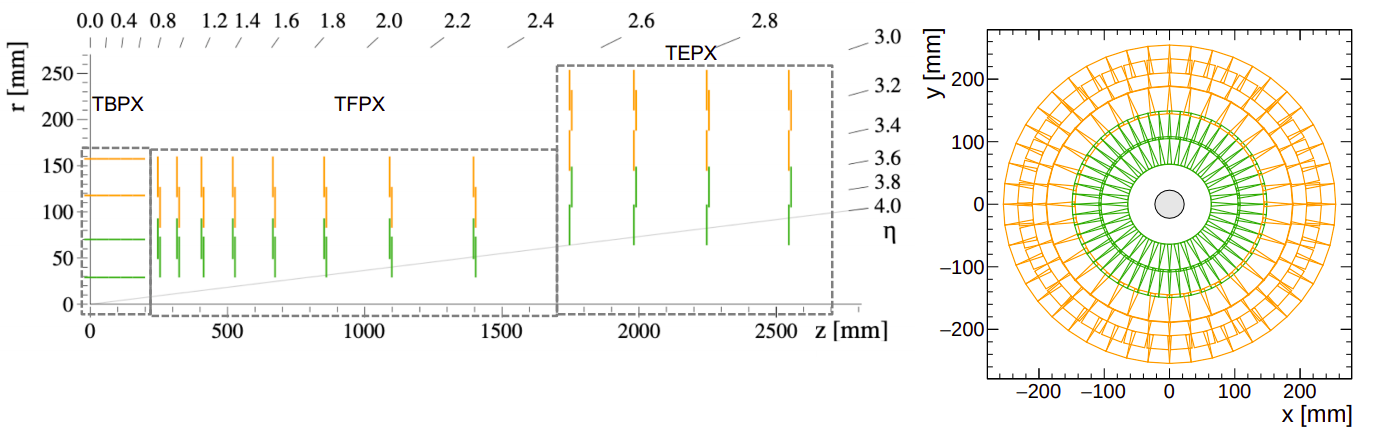
\includegraphics[width=1 \columnwidth]{./tepx_tt.png}
  \caption{ \onehalfspacing Left: A layout of the CMS Phase II inner tracker showing four TEPX disks, eight TFPX disks and four barrel layers. Right: Diagram showing one double disk of TEPX with five rings \cite{Klein:2017nke}.}
  \label{fig:CMS}
\end{figure}


\begin{figure}[H]
  \centering
  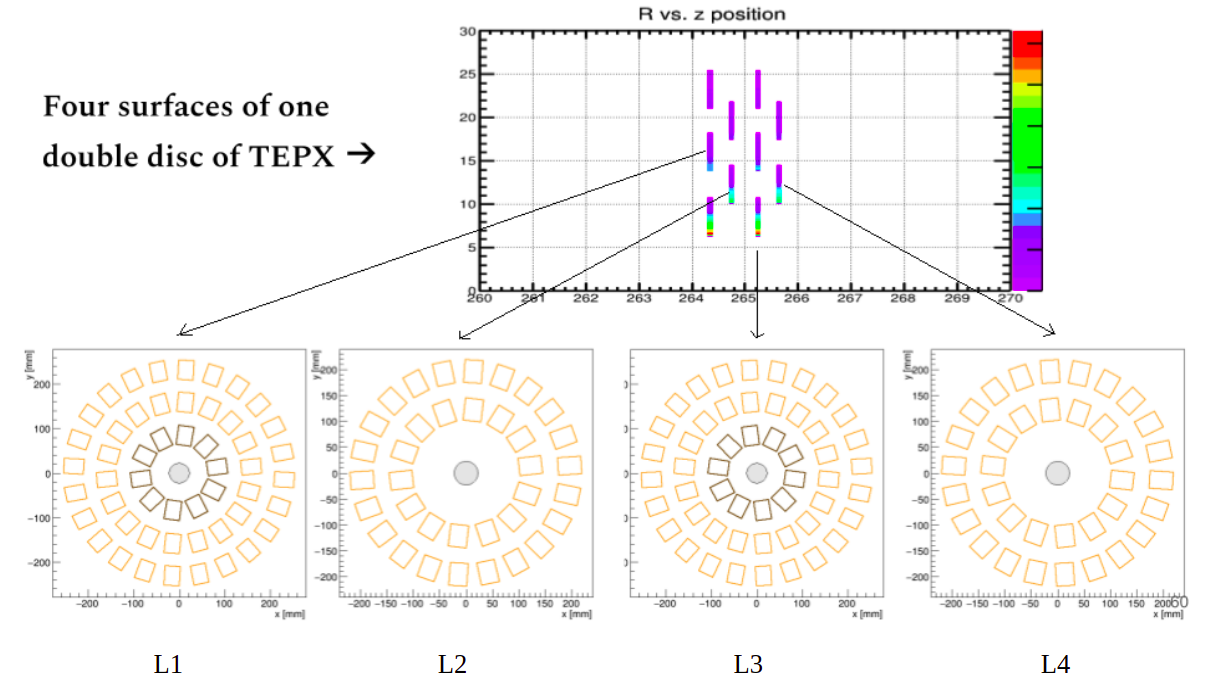
\includegraphics[width=1 \columnwidth]{./fourlayers.png}
  \caption{ \onehalfspacing Fours layers of one double disk of TEPX showing module arrangement in rings for each layer. Ring 1, 2, 3, 4 and 5 consists of 20, 28, 36, 44 and 48 modules respectively. }
  \label{fig:CMS}
\end{figure}

%\subsection{Expected improvements in luminosity measurement with the new TEPX detector}
\subsection{Phase II CMS simulation samples}

 Simulated data samples for Phase II include full CMS detector description and uses official CMS software (CMSSW) version $10-6-0-patch2$ which calls GEANT4 for particle and energy deposit simulation as well as for reconstruction \cite{Agostinelli:2002hh}. These samples contain single-neutrino event overlaid with a variable number of minimum-bias events (events with any amount of real energy detected in CMS) to simulate different pileup values. The statistics for samples with average pileup values from 0.5 to 2 is 500000 events per step and for average pileup values between 10 and 200, statistics is 100000. 

\begin{table}[htbp]
  \centering
  \caption{Phase II upgrade of CMS tracker datasets}
  \label{tab:sample}
  \begin{tabular}{ccc}
    \hline
    \textbf{pileup} & \textbf{Total number of events} & \textbf{Dataset name} \\
    \hline
    noPU  & 500000 & /RelValNuGun/CMSSW_10_6_0_patch2-106X_upgrade2023_realistic_v3_2023D42noPU-v1/GEN-SIM-RECO \\
     0.5& 500000 &  /RelValNuGun/CMSSW_10_6_0_patch2-PU25ns_106X_upgrade2023_realistic_v3_2023D42PU0p5-v1/GEN-SIM-RECO\\
     1&  & 500000 &   /RelValNuGun/CMSSW_10_6_0_patch2-PU25ns_106X_upgrade2023_realistic_v3_2023D42PU1-v1/GEN-SIM-RECO\\
     1.5 & 500000 &   /RelValNuGun/CMSSW_10_6_0_patch2-PU25ns_106X_upgrade2023_realistic_v3_2023D42PU1p5-v1/GEN-SIM-RECO\\
     2&  &  500000 &   /RelValNuGun/CMSSW_10_6_0_patch2-PU25ns_106X_upgrade2023_realistic_v3_2023D42PU2-v1/GEN-SIM-RECO\\
     10&  &  100000&   /RelValNuGun/CMSSW_10_6_0_patch2-PU25ns_106X_upgrade2023_realistic_v3_2023D42PU10-v1/GEN-SIM-RECO\\
      30&  &  100000&   /RelValNuGun/CMSSW_10_6_0_patch2-PU25ns_106X_upgrade2023_realistic_v3_2023D42PU30-v1/GEN-SIM-RECO\\
     50&  &  100000&   /RelValNuGun/CMSSW_10_6_0_patch2-PU25ns_106X_upgrade2023_realistic_v3_2023D42PU50-v1/GEN-SIM-RECO \\
     100&  & 100000 & /RelValNuGun/CMSSW_10_6_0_patch2-PU25ns_106X_upgrade2023_realistic_v3_2023D42PU100-v2/GEN-SIM-RECO\\
      140&  &  99600&  /RelValNuGun/CMSSW_10_6_0_patch2-PU25ns_106X_upgrade2023_realistic_v3_2023D42PU140-v2/GEN-SIM-RECO\\
     200&  &  100000&  /RelValNuGun/CMSSW_10_6_0_patch2-PU25ns_106X_upgrade2023_realistic_v3_2023D42PU200-v1/GEN-SIM-RECO\\
    %\hline
  \end{tabular}
\end{table}


$/RelValNuGun/CMSSW_10_6_0_patch2-PU25ns_106X_upgrade2023_realistic_v3_2023D42PU200-v1/GEN-SIM-RECO$
This dataset represents a simulated event sample generated using the CMS software framework, CMSSW, for the phase-2 upgrade of the CMS detector at the Large Hadron Collider (LHC). 

\begin{itemize}

\item RelValNuGun: This refers to the type of generated events in this dataset. "RelVal" is short for "Release Validation," meaning that this sample is used for validating the performance of the CMS software release. "NuGun" refers to the specific event generator setup used for this dataset, which is a neutrino gun. In this setup, neutrinos are produced uniformly throughout the detector, providing a simple event topology for testing the software and detector response.

\item $CMSSW_10_6_0_patch2$: This refers to the version of the CMS Software (CMSSW) used to generate and process the dataset. In this case, it is version 10.6.0 with patch 2 applied, containing specific software improvements or bug fixes.

\item $PU25ns_106X_upgrade2023_realistic_v3_2023D42PU200$: This part contains several details about the dataset conditions:

\item PU25ns: This indicates that the dataset includes simulated pileup events with an average of 25 collisions per bunch crossing, separated by 25 nanoseconds.
\item 106X: This refers to the software release cycle (10.6.X) used for this dataset.
\item $upgrade2023_realistic_v3$: This specifies that the dataset is for the planned 2023 upgrade of the CMS detector, using a "realistic" geometry and conditions version 3, which simulates the expected detector performance and environment.
\item 2023D42PU200: This is a specific identifier for the simulated detector layout (D42) and conditions for the 2023 upgrade, with an emphasis on the 200 pileup events included in the simulation.
GEN-SIM-RECO: These are the processing steps applied to the dataset:

\item GEN: The "Generator" step, where the initial particle-level events are generated using Monte Carlo methods.
\item SIM: The "Simulation" step, where the detector's response to the generated particles is simulated, taking into account the detector geometry, materials, and electronics.
\item RECO: The "Reconstruction" step, where the simulated detector hits are processed to reconstruct the physics objects (e.g., particles and their trajectories), which are then used for further analysis.

This dataset represents a set of simulated neutrino gun events, generated and processed with the CMS software version $10.6.0_patch2$, for the phase-2 upgrade of the CMS detector in 2023. The dataset includes realistic detector geometry and conditions, and 25ns pileup events, with an emphasis on 200 pileup events. The dataset has undergone the generation, simulation, and reconstruction steps, making it suitable for validation and analysis tasks.

\end{itemize}


\begin{table}[htbp]
  \centering
  \caption{Events per file for each pileup}
  \label{tab:sample}
  \begin{tabular}{ccc}
     \textbf{Pileup} & \textbf{Events per file} \\
     \hline
     noPU &   2000\\
     0.5 &   2000\\
     1&    1800\\
      1.5&  1500\\
      2&   1400\\
     10&    500\\
     30&    200\\
      50&   100\\
      100&   100\\
     140&    100\\
       200&    100\\
  \end{tabular}
\end{table}



\begin{table}[htbp]
  \centering
  \caption{Events processed for each pileup}
  \label{tab:sample}
  \begin{tabular}{ccc}
     \textbf{Pileup} & \textbf{Number of events processed} \\
     \hline
     noPU & 10000  \\
     0.5 &  100600 \\
     1&    87400\\
      1.5& 74900 \\
      2&  66200 \\
     10&   21800 \\
     30&    10000\\
      50&   5000\\
      100&   5000\\
     140&    5000\\
       200&    5000\\
  \end{tabular}
\end{table}


\section{Luminosity determination using TEPX - counting clusters/coincidences}

Luminosity determination using PCC method for Phase II HL-LHC will be based on counting the number of clusters in TEPX Disk 4 Ring 1. The innermost ring of the last disk of TEPX (D4R1) is located at 2.65 m away from the interaction point that is beyond the tracking acceptance ($|\eta| = 4$) and as this region has few tracking points, it can be solely used for the purpose of luminosity measurement by using the full available trigger rate and bandwidth.

\begin{figure}[H]
  \centering
  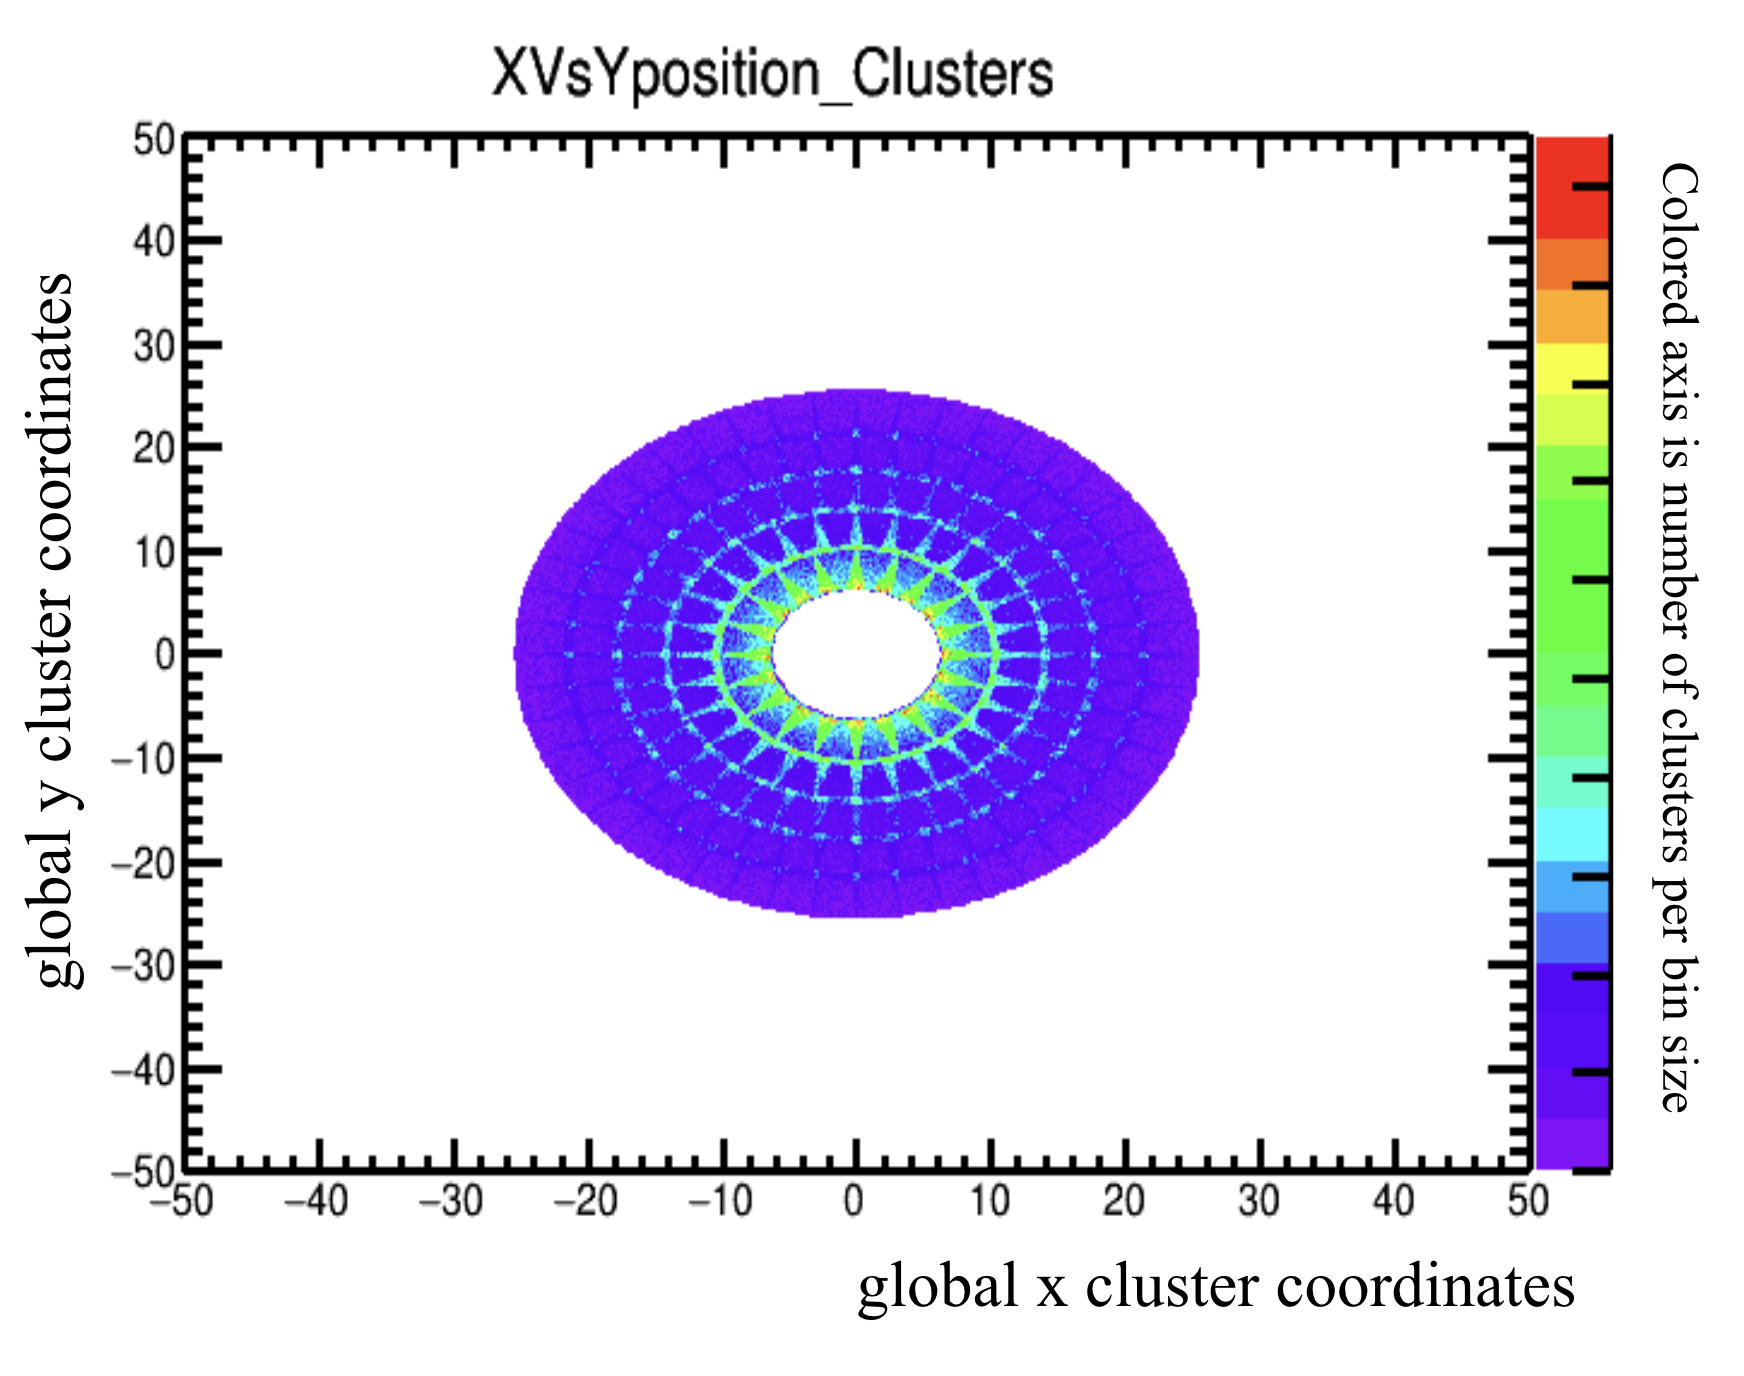
\includegraphics[width=1\columnwidth]{ashish_thesis/tepx_clusters.png}
  \caption{TEPX cluster map in the XY plane for pileup 200 simulated sample. Map showing coordinates of TEPX clusters in CMS global coordinate system. It shows clusters in one TEPX disk consisting of 5 rings. Hot regions are showing the module overlap for all rings (red, orange, green, yellow). Number of x bins is 1000, x bins range from -50 to 50. x bin size is 0.1 cm. Number of y bins is 1000, y bins range from -50 to 50. y bin size is 0.1 cm.}
  \label{fig:tepx_cl}
\end{figure}


\begin{figure}[H]
  \centering
  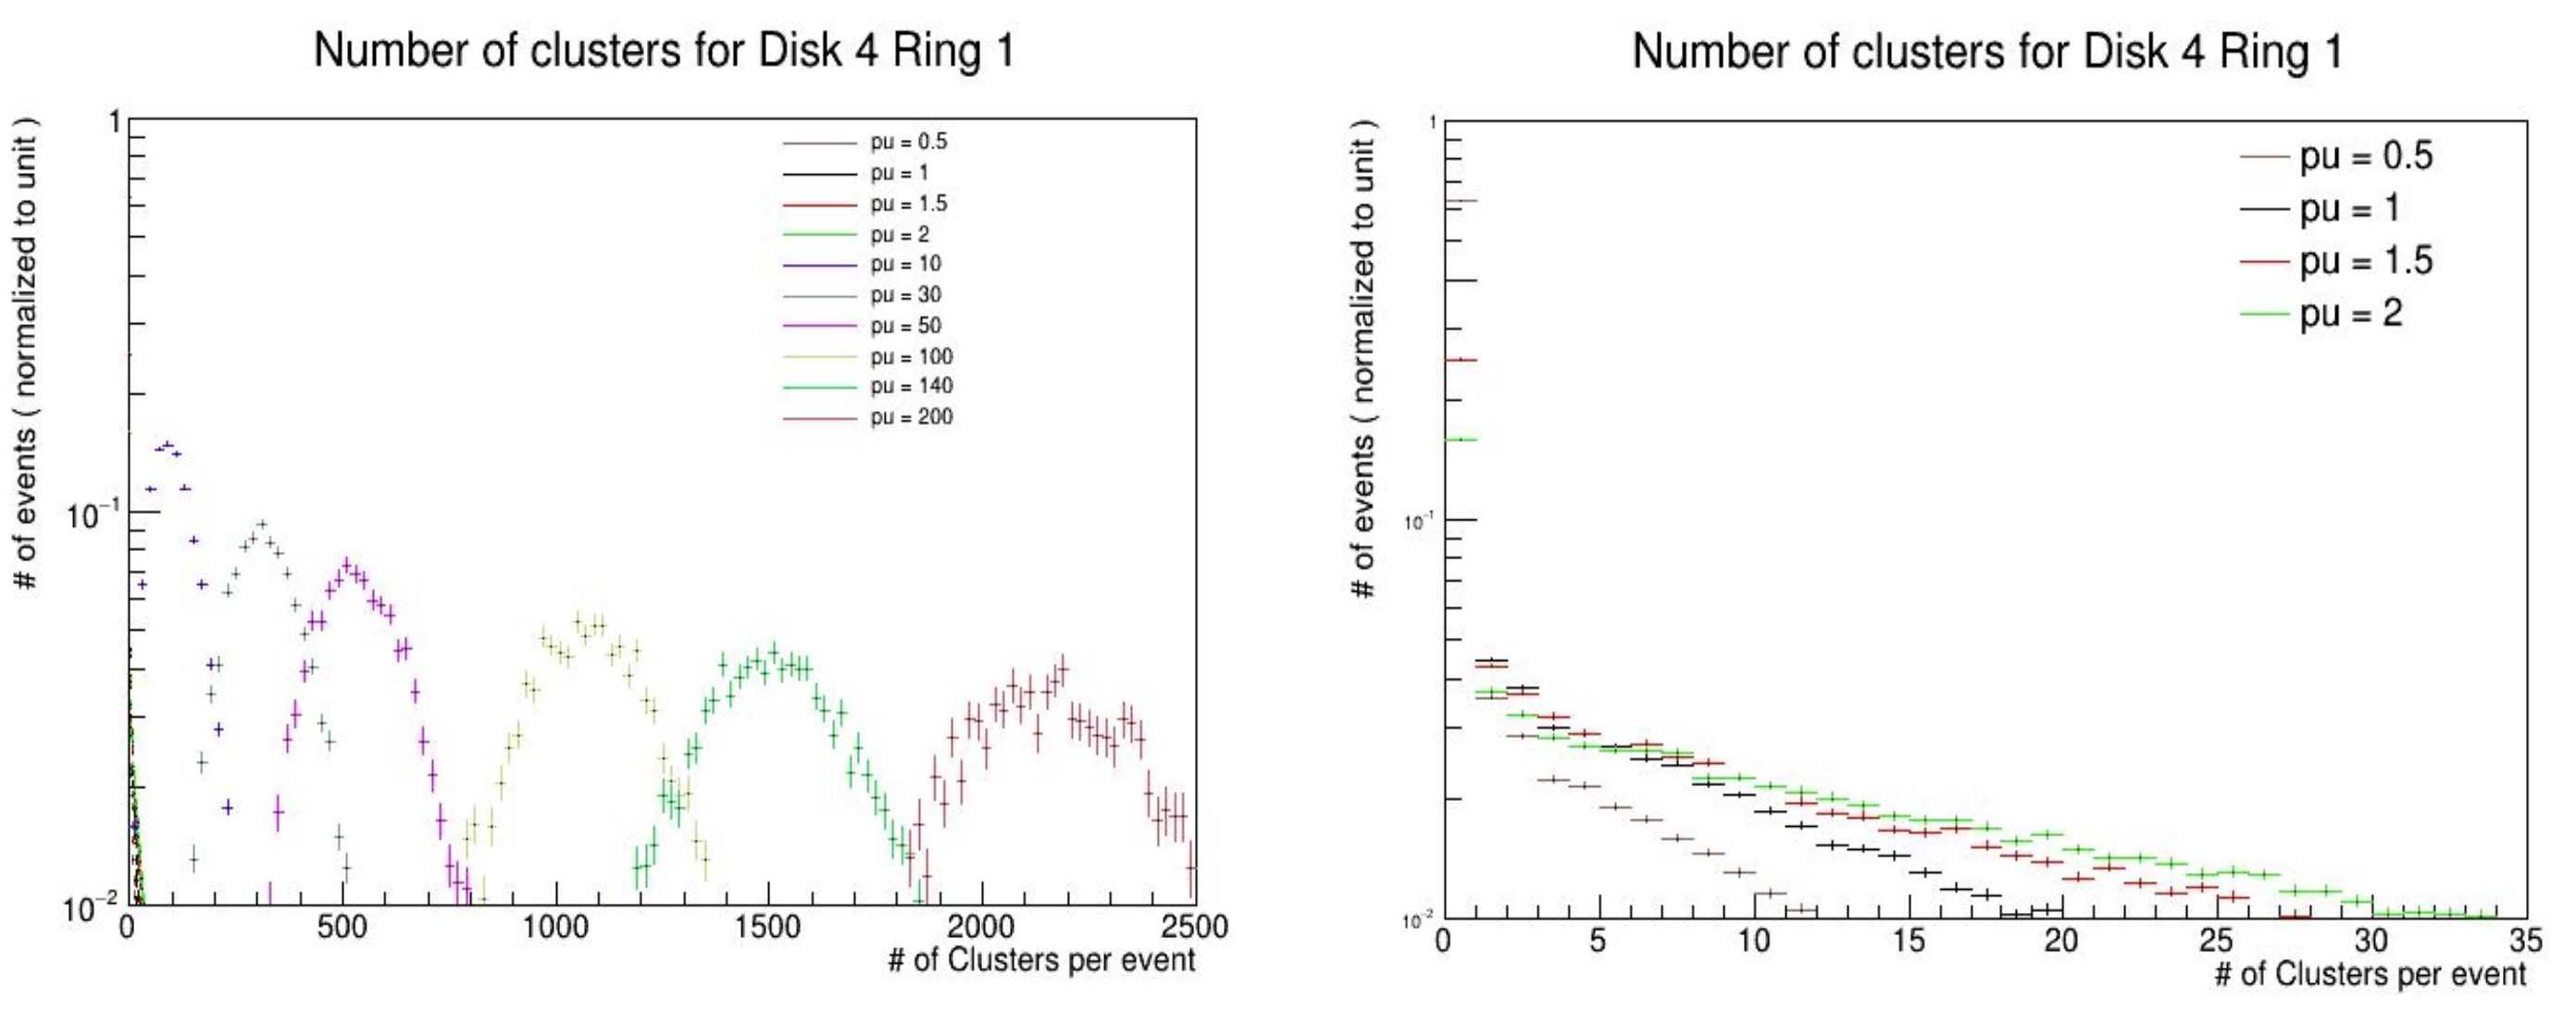
\includegraphics[width=1\columnwidth]{ashish_thesis/tepx_D4R!_clusters._allpupng.png}
  \caption{Left: Distribution of number of clusters for TEPX Disk 4 Ring 1 for all pileup values. Right: Distribution of number of clusters for TEPX Disk 4 Ring 1 for all low pileup values. }
  \label{fig:tepx_cl_allPU}
\end{figure}

\begin{figure}[H]
  \centering
  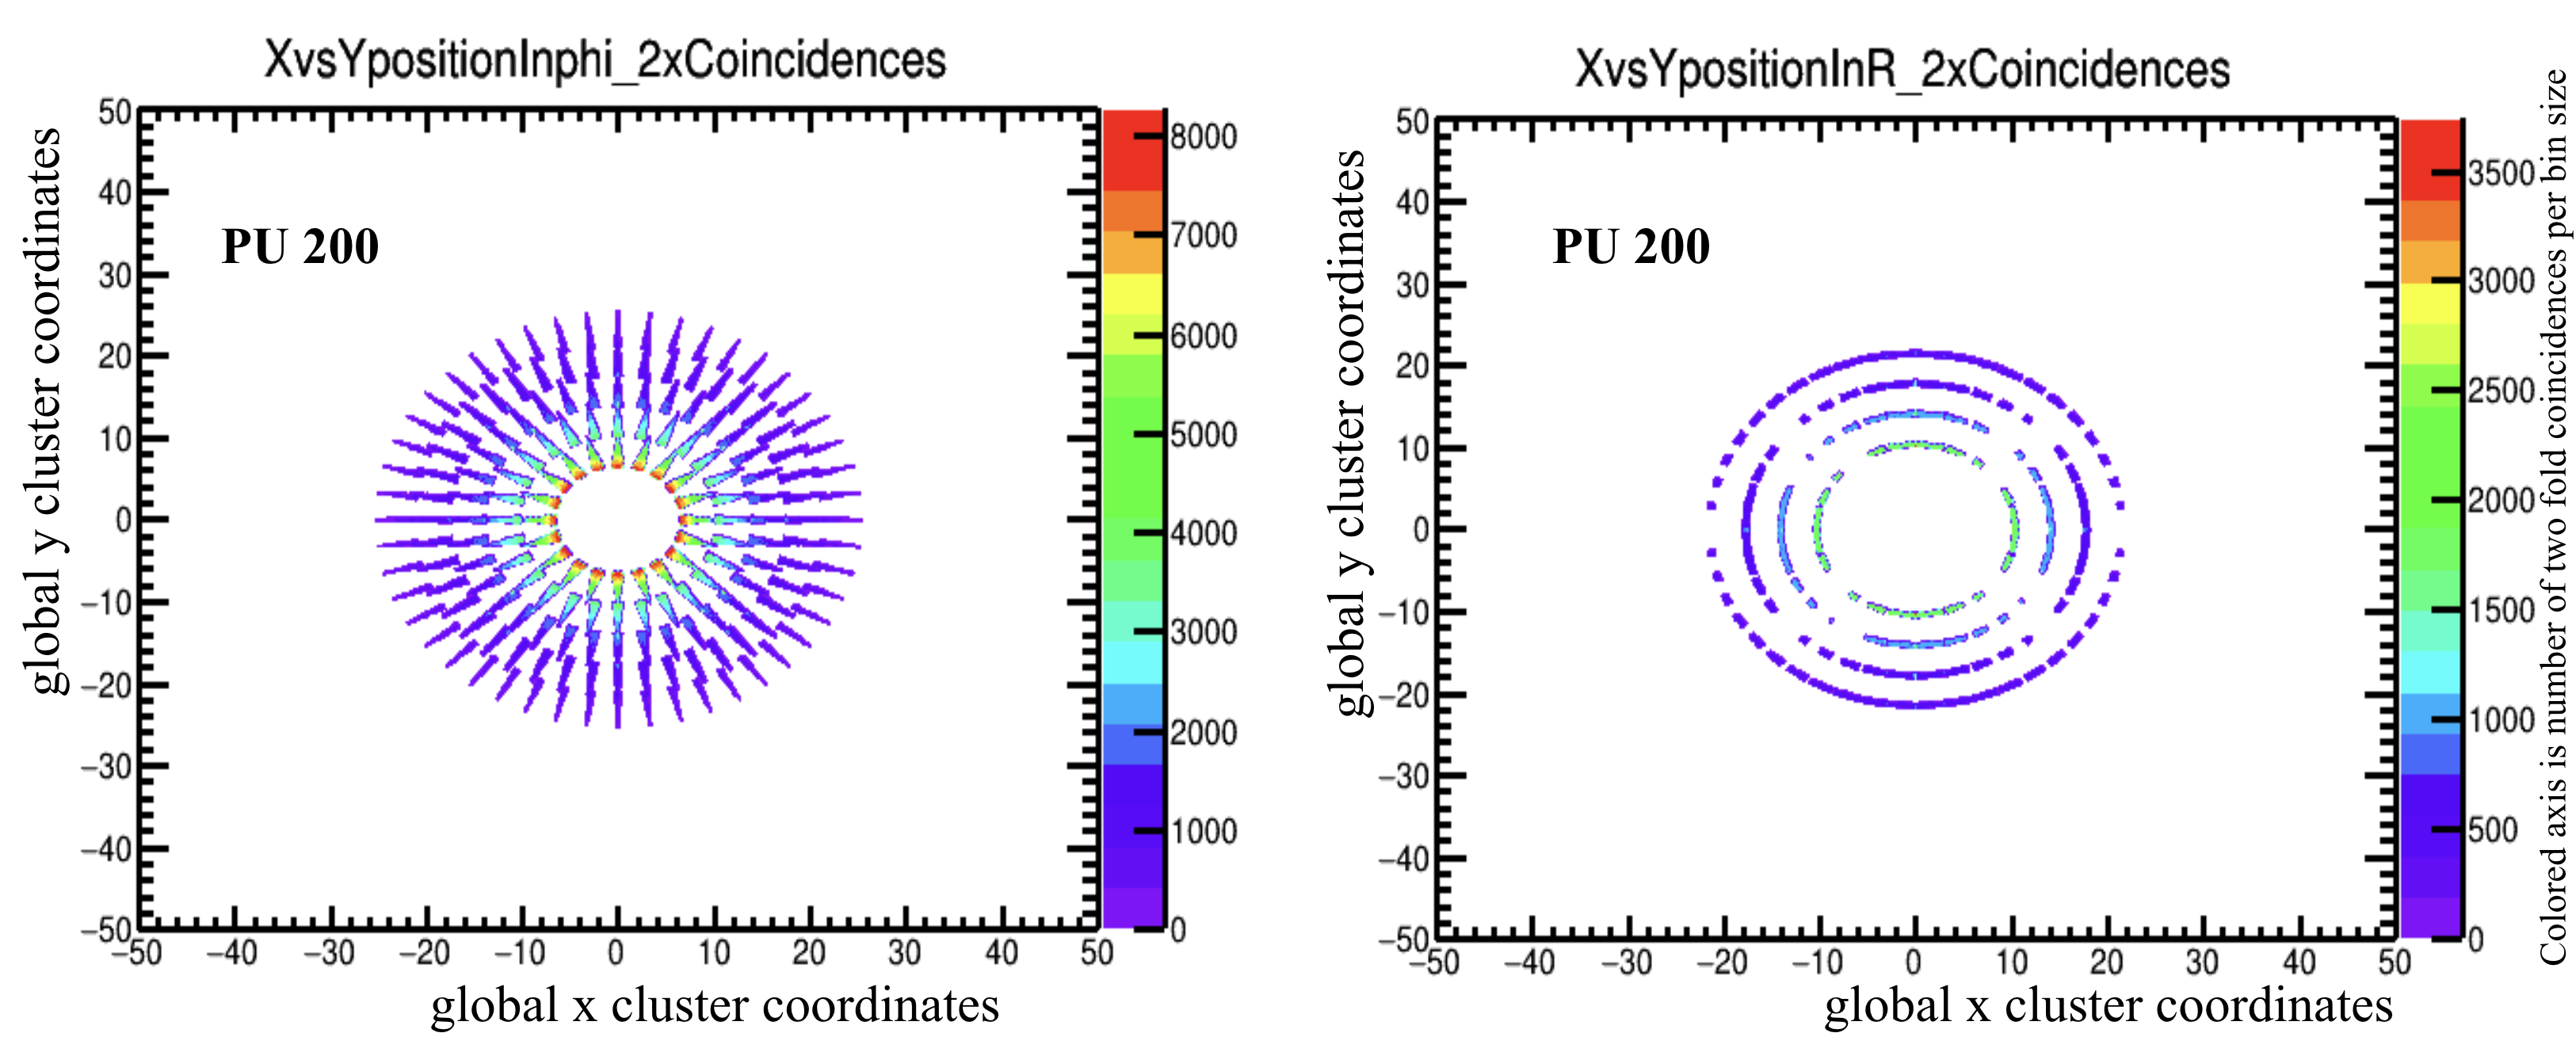
\includegraphics[width=1\columnwidth]{ashish_thesis/tepx_coincidences.png}
  \caption{Left: TEPX coincidences in phi map in the XY plane for pileup 200 simulated sample. Right:TEPX coincidences in R map in the XY plane for pileup 200 simulated sample. Number of x bins is 1000, x bins range from -50 to 50. x bin size is 0.1 cm and Number of y bins is 1000, y bins range from -50 to 50. y bin size is 0.1 cm.}
  \label{fig:tepx_coinc}
\end{figure}


\begin{figure}[H]
  \centering
  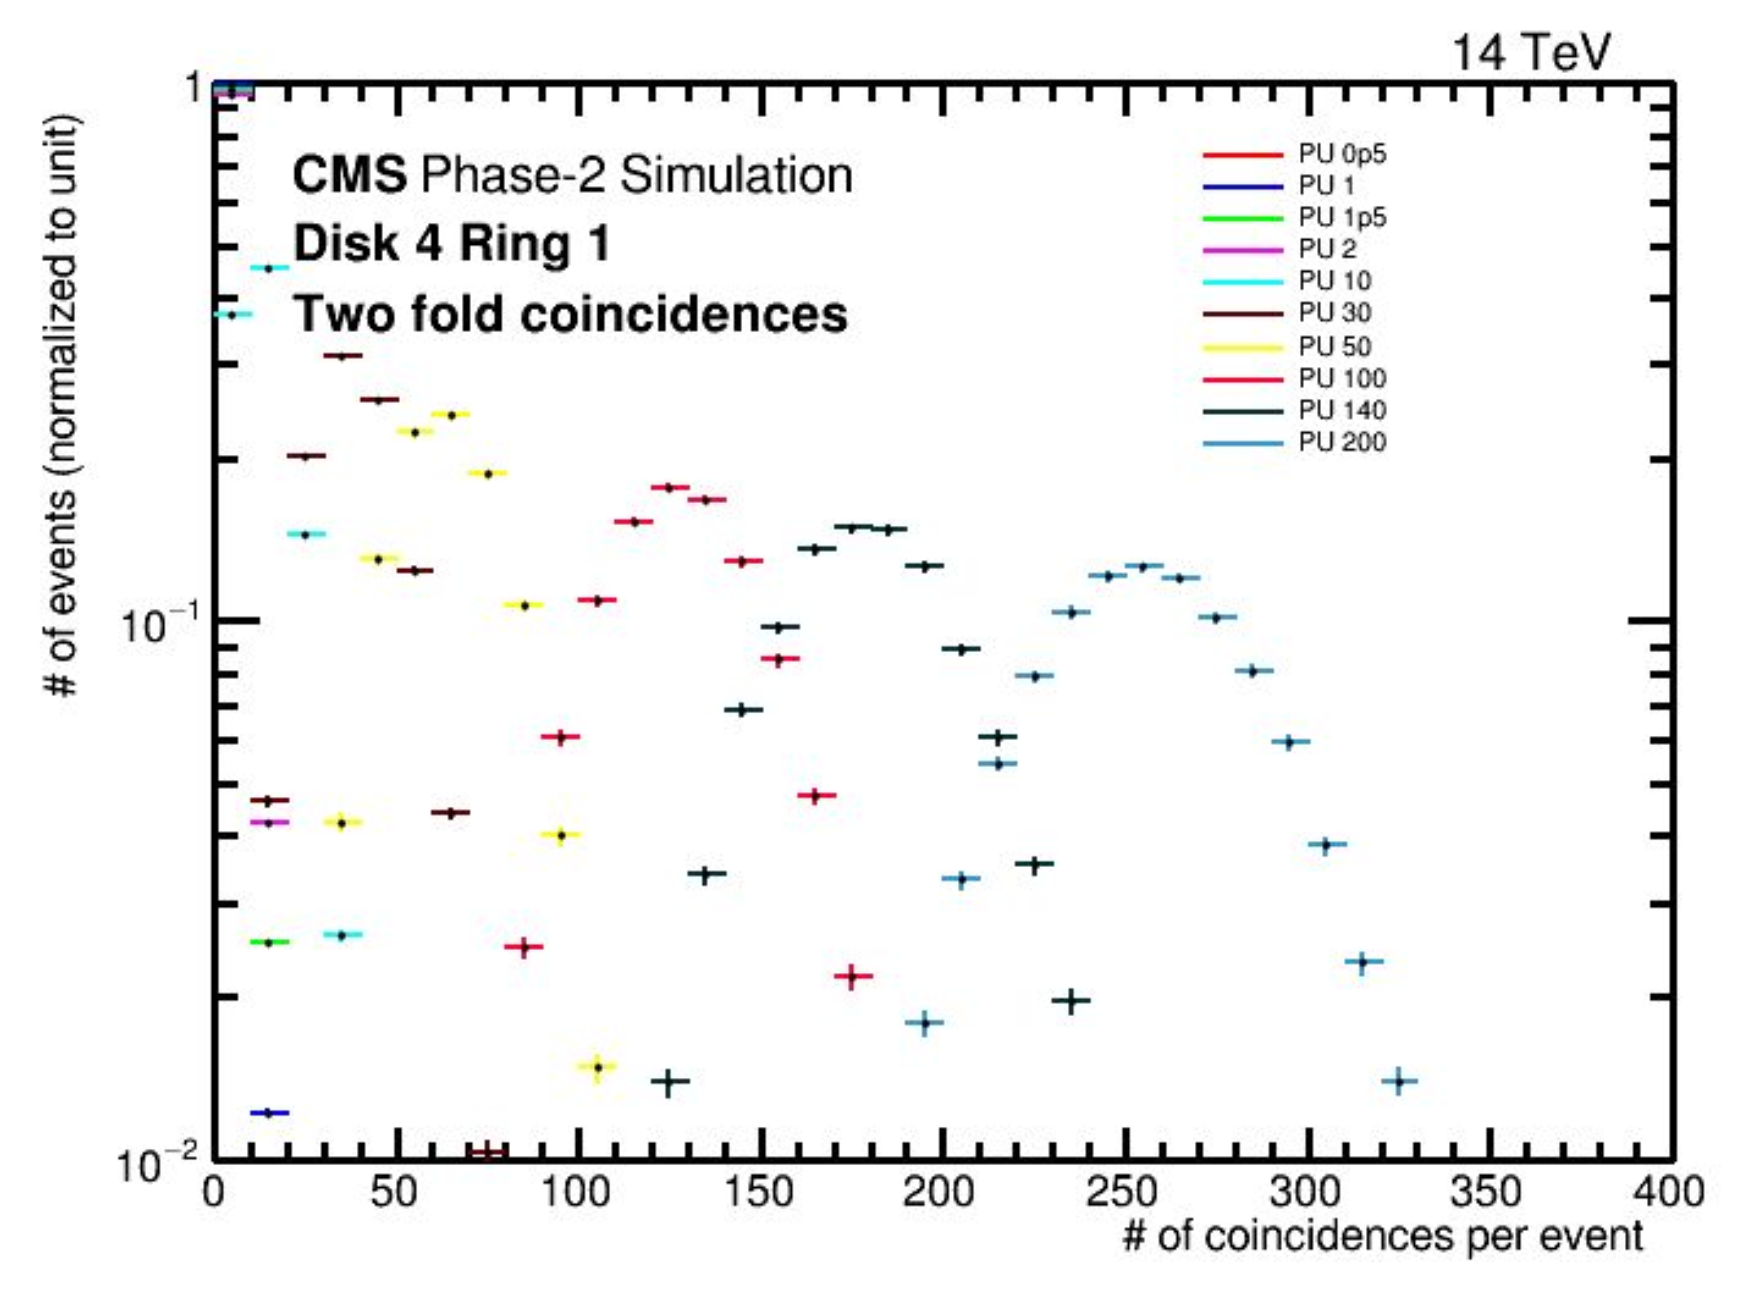
\includegraphics[width=1\columnwidth]{ashish_thesis/tepx_D4R1_coin_allpu.png}
  \caption{Left: Distribution of number of two fold coincidences for TEPX Disk 4 Ring 1 for all pileup values. Right: Distribution of number of two fold coincidences for TEPX Disk 4 Ring 1 for all low pileup values.}
  \label{fig:tepx_coin_allPU}
\end{figure}


\begin{figure}[H]
  \centering
  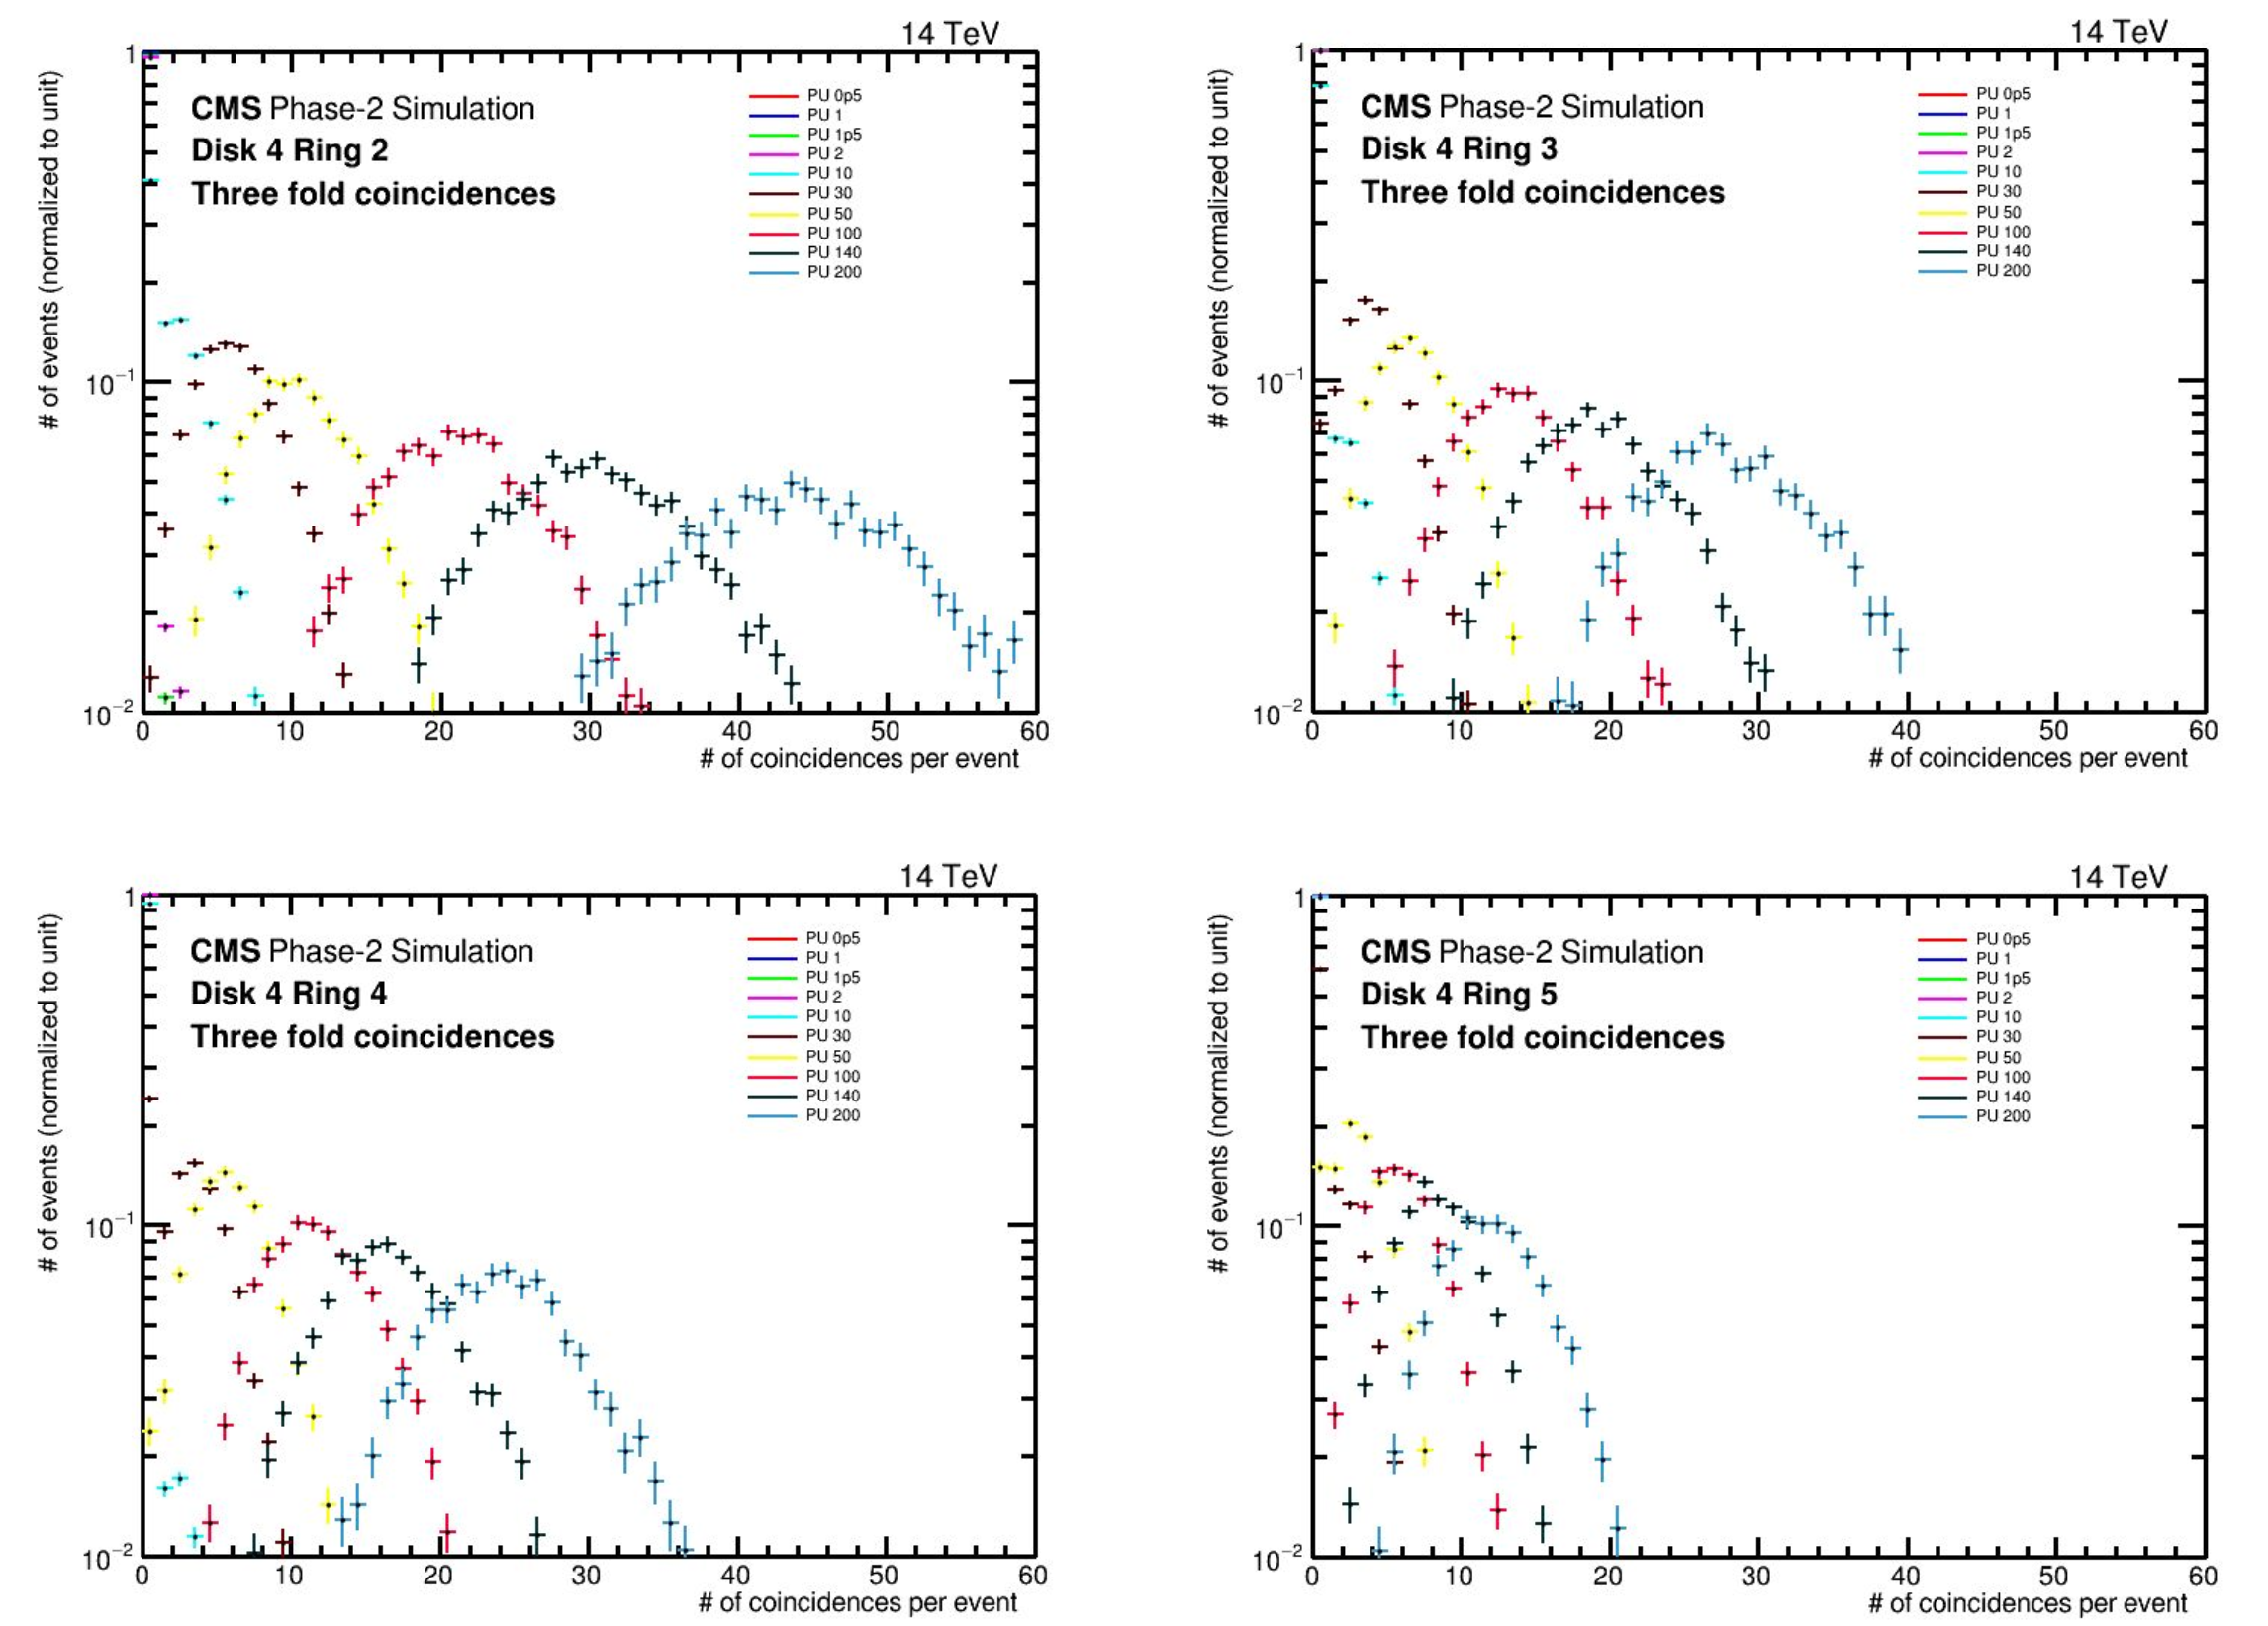
\includegraphics[width=1\columnwidth]{ashish_thesis/tepx_D4_3foldcoin_allpu.png}
  \caption{Distribution of number of three fold coincidences for TEPX Disk 4 all rings for all pileup values.}
  \label{fig:tepx_3foldcoin_allPU}
\end{figure}

\begin{figure}[H]
  \centering
  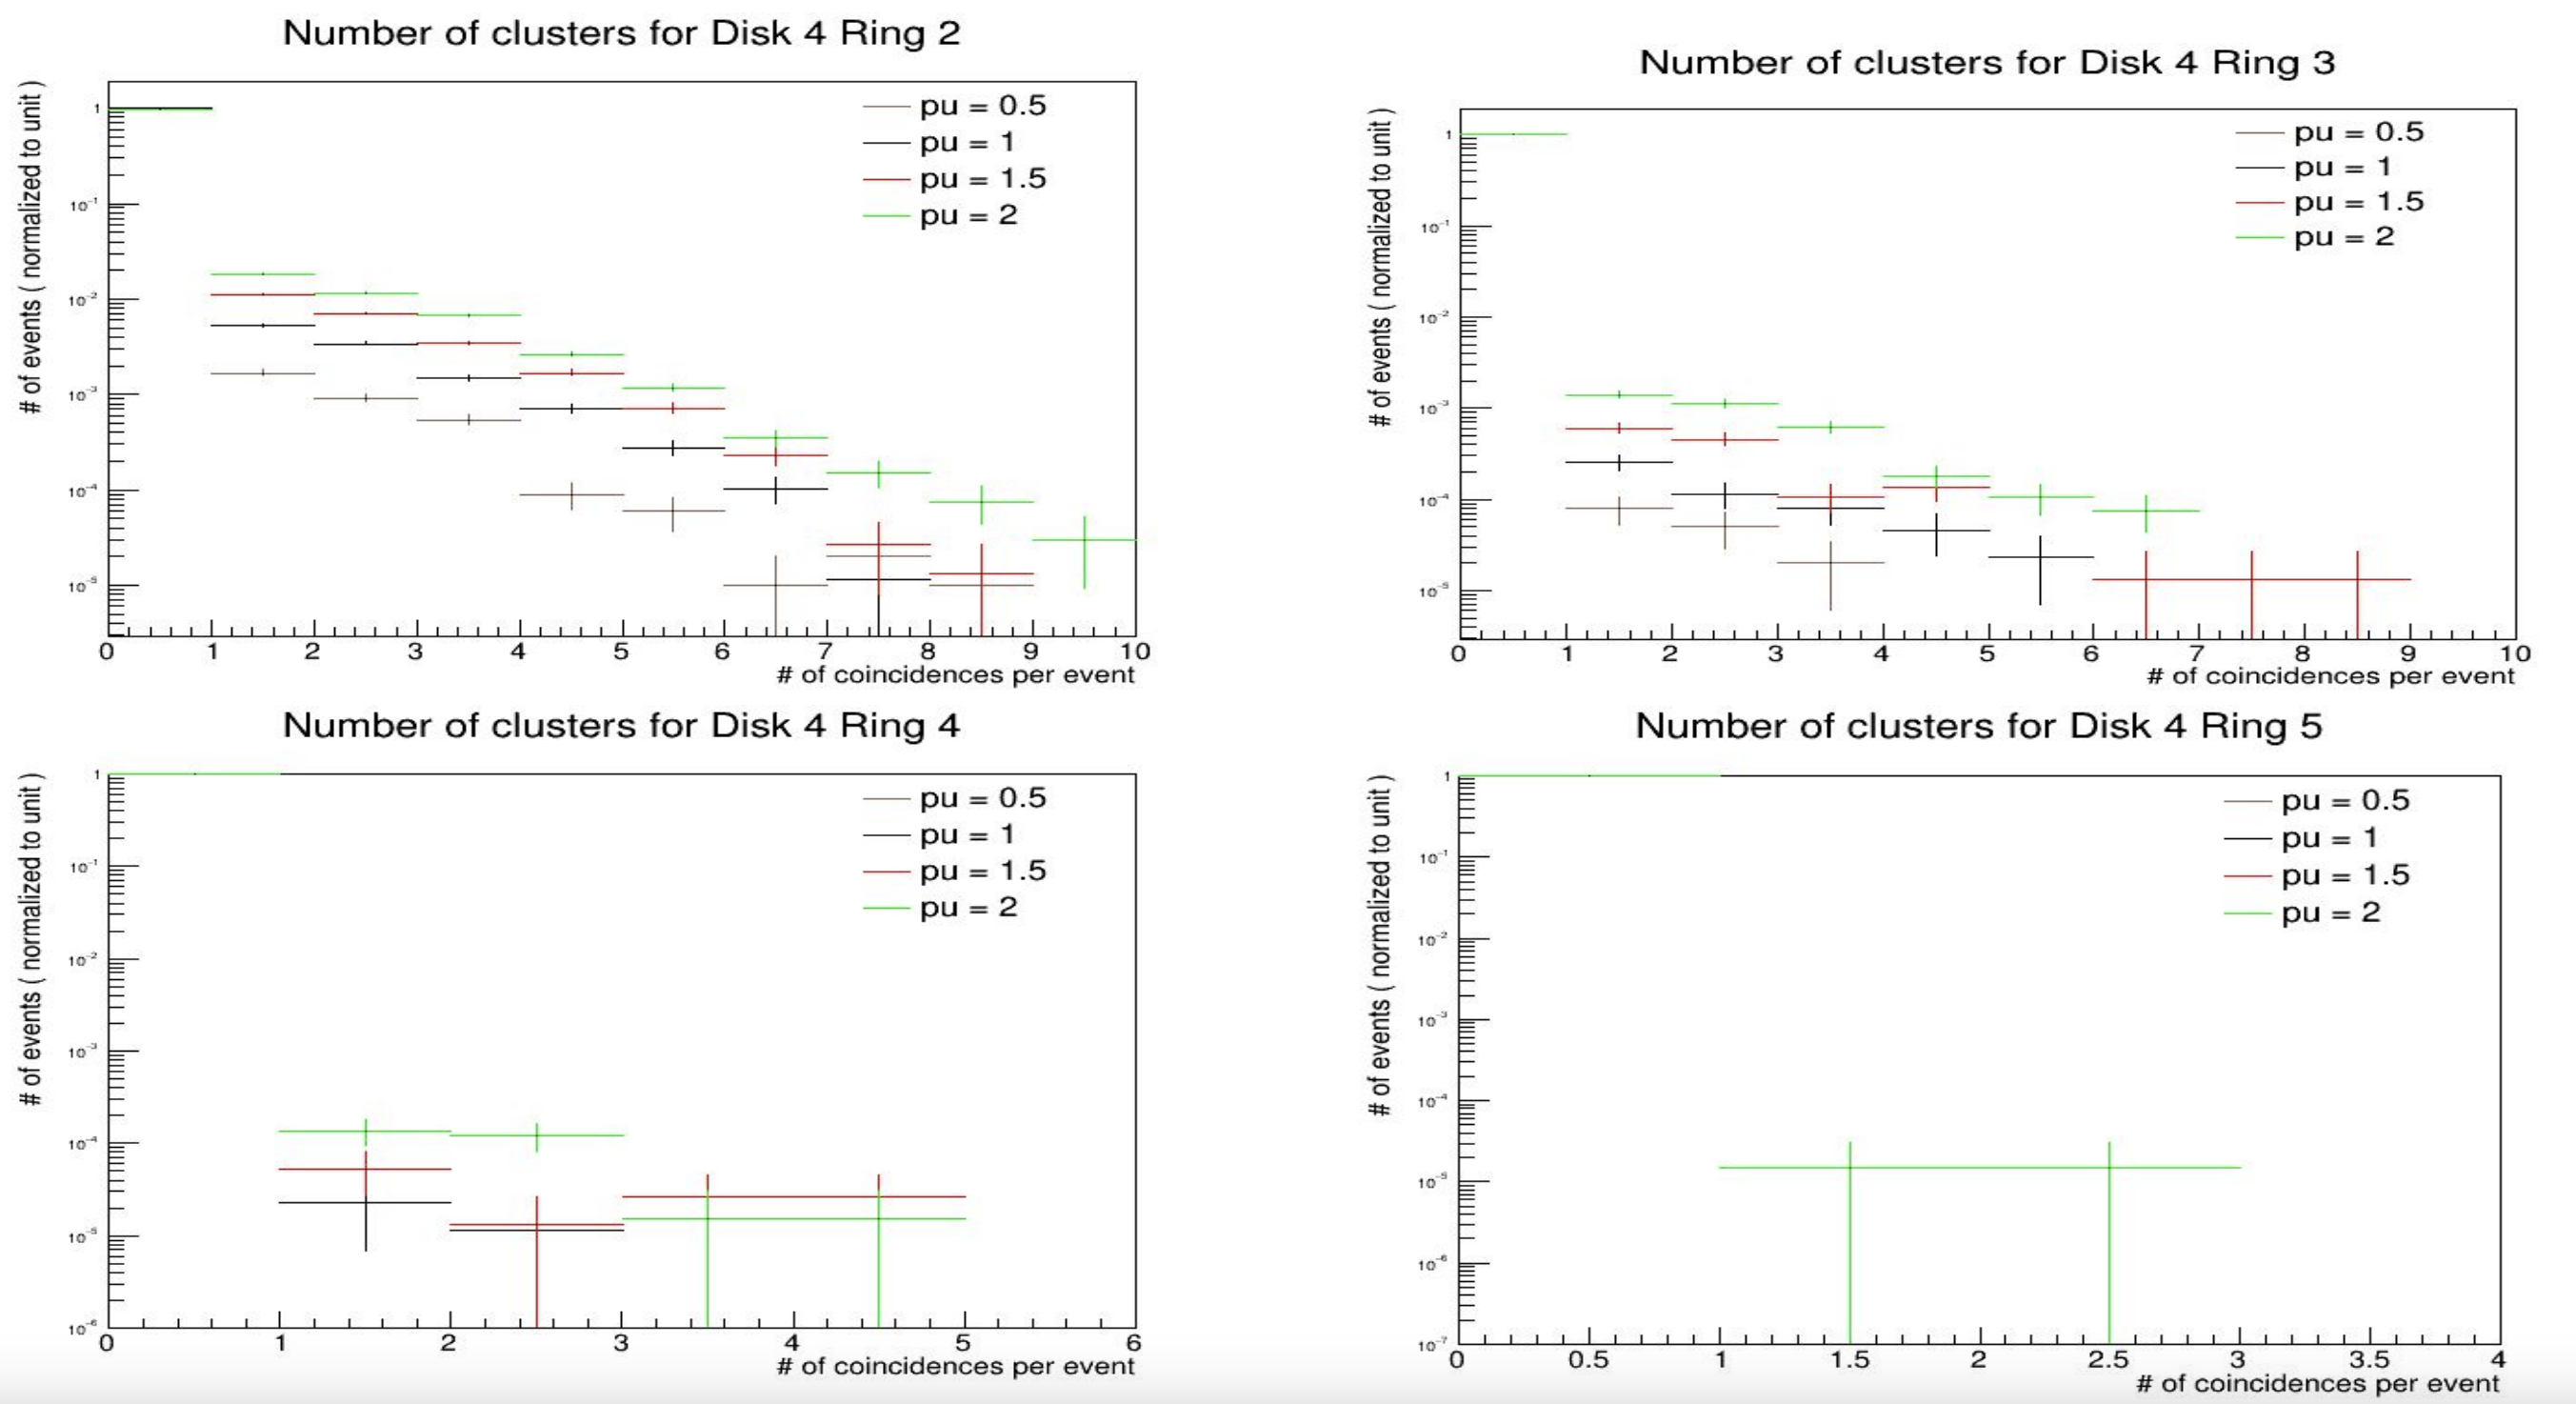
\includegraphics[width=1\columnwidth]{ashish_thesis/tepx_D4_3foldcoin_lowpu.png}
  \caption{Distribution of number of three fold coincidences for TEPX Disk 4 all rings for low pileup values.}
  \label{fig:tepx_3foldcoin_allPU}
\end{figure}

\subsubsection{Old algorithm for counting TEPX two fold coincidences}

\begin{figure}[!htp]
\centering
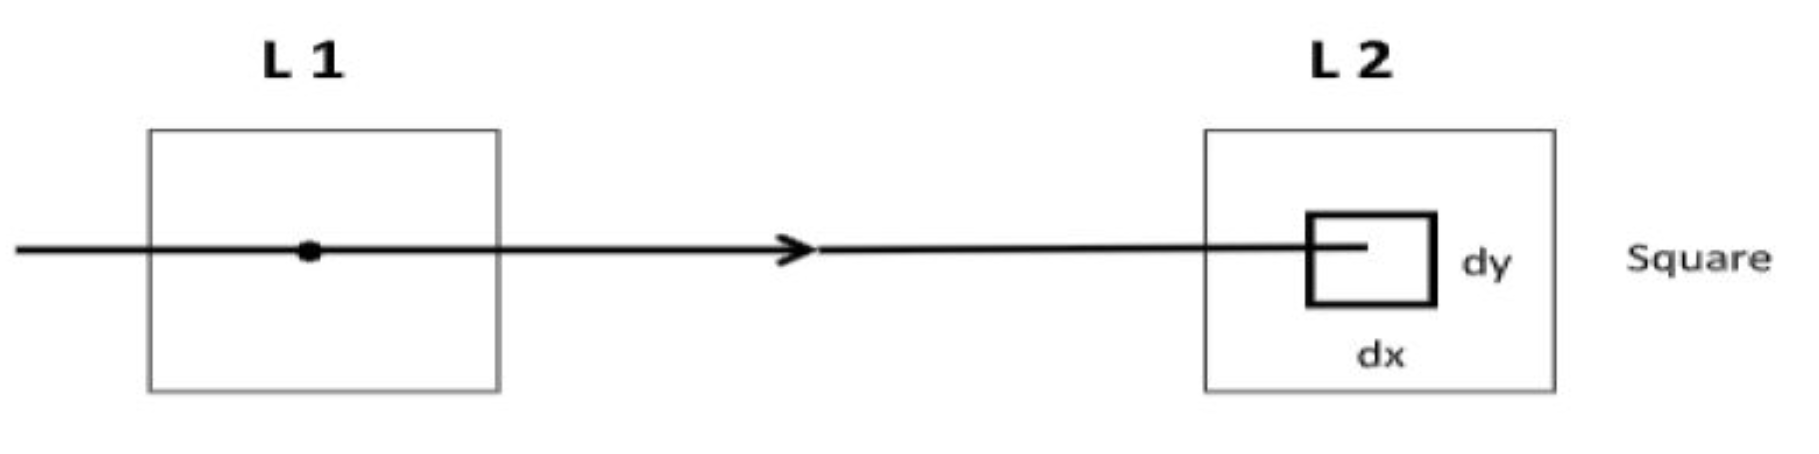
\includegraphics[width=1\textwidth]{ashish_thesis/oldvariable_xy.png}
\caption{%
   Old X, Y variables used for defining two fold coincidences clusters in phi.
}
\label{fig:oldvar_xy}
\end{figure}


\begin{figure}[!htp]
\centering
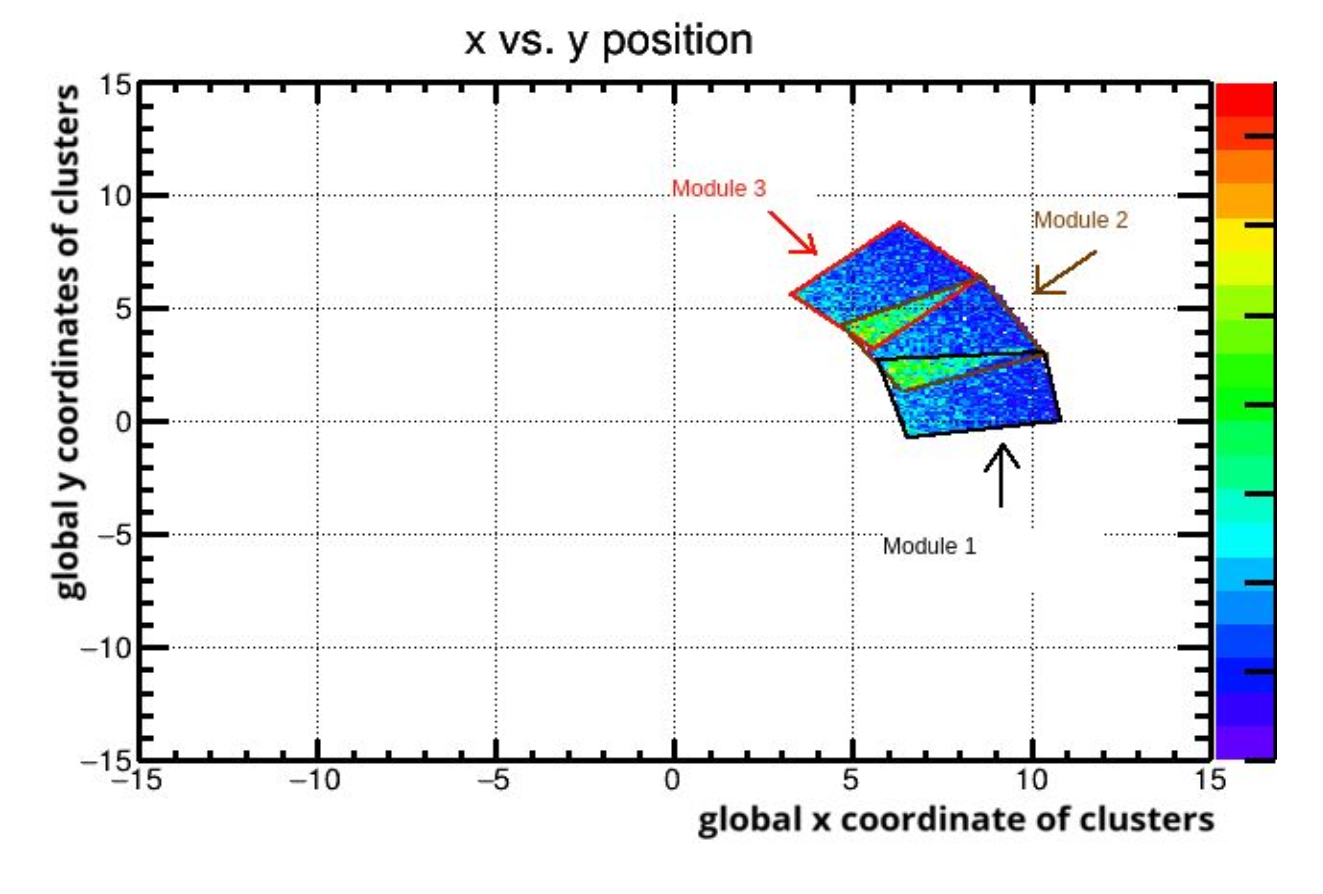
\includegraphics[width=1\textwidth]{ashish_thesis/overlap_modules2_Ring1.png}
\caption{%
 XY cluster map showing module overlap within the same ring in a disk that gives rise to two fold coincidences in phi.
}
\label{fig:overlap_2foldinphi}
\end{figure}



\begin{figure}[!htp]
\centering
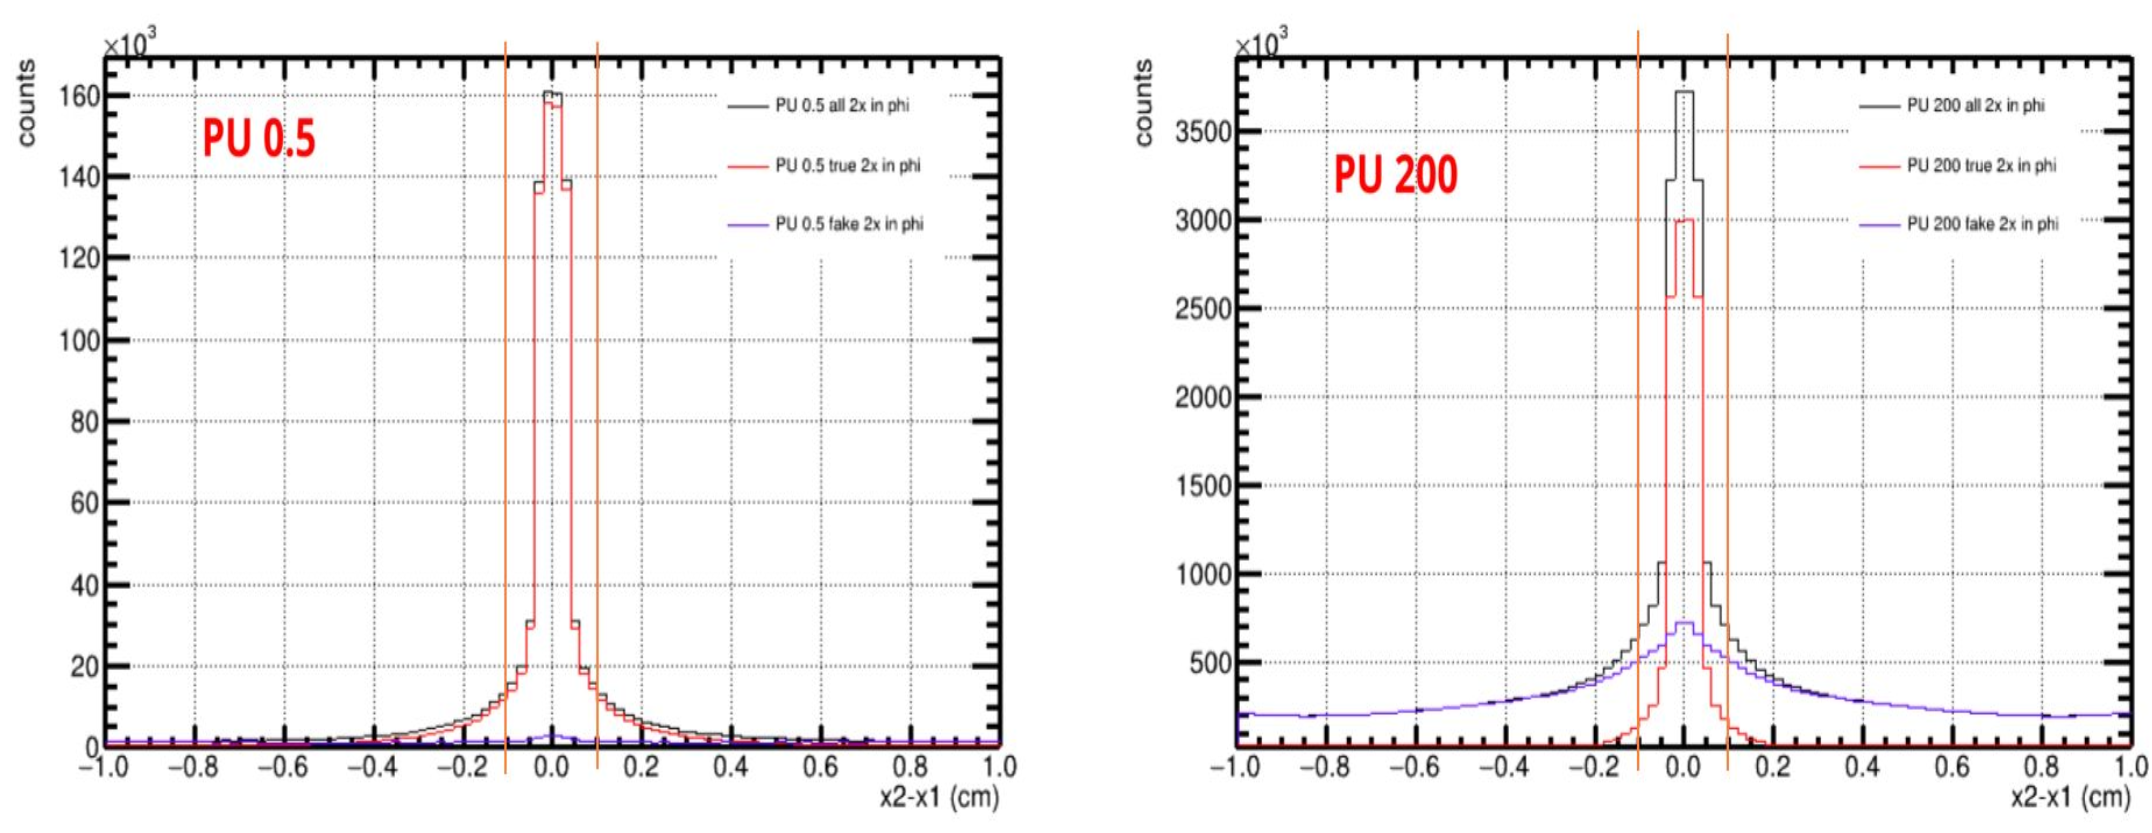
\includegraphics[width=1\textwidth]{ashish_thesis/twofoldcoin_inphi_PU0p5_200.png}
\caption{%
 Separation between X coordinates of two clusters for pileup 0.5 and 200 showing distribution total, true and fake two fold coincidences in phi.
}
\label{fig:dx_twofold}
\end{figure}



\begin{figure}[!htp]
\centering
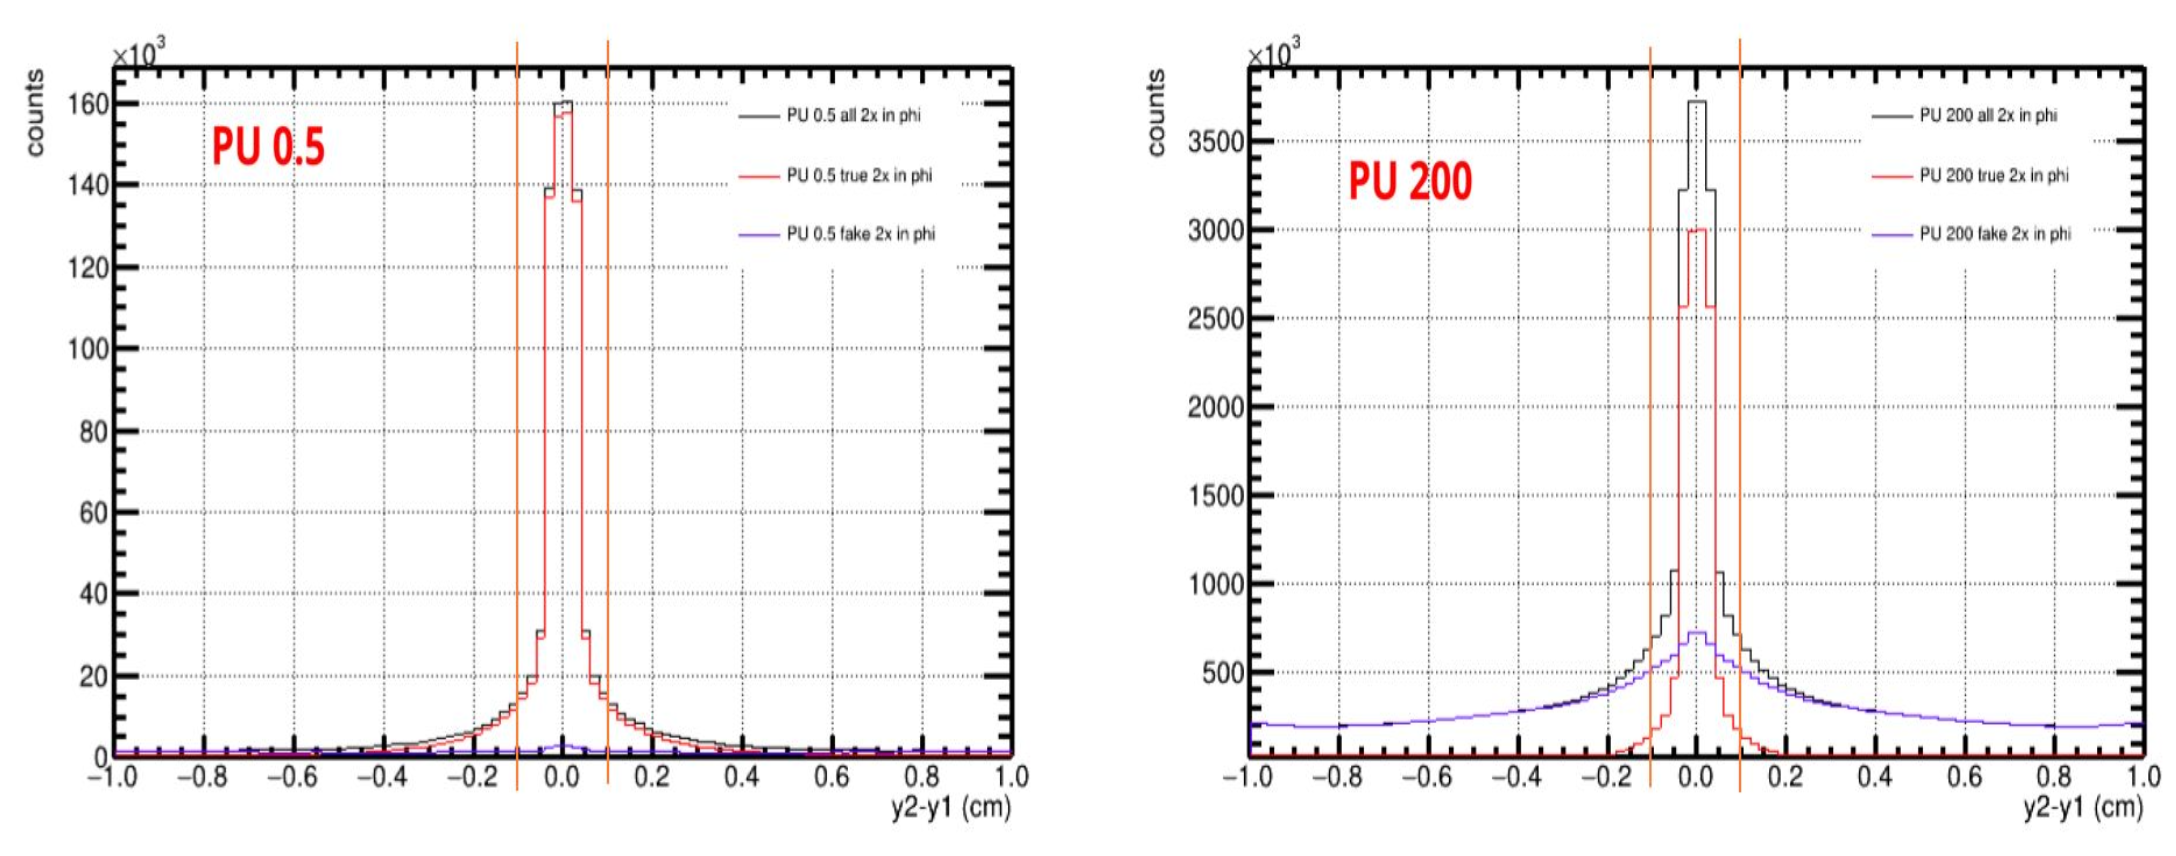
\includegraphics[width=1\textwidth]{ashish_thesis/twofoldcoin_cluster_y.png}
\caption{%
    Separation between Y coordinates of two clusters for pileup 0.5 and 200 showing distribution total, true and fake two fold coincidences in phi.
}
\label{fig:dy_twofold}
\end{figure}




\begin{figure}[!htp]
\centering
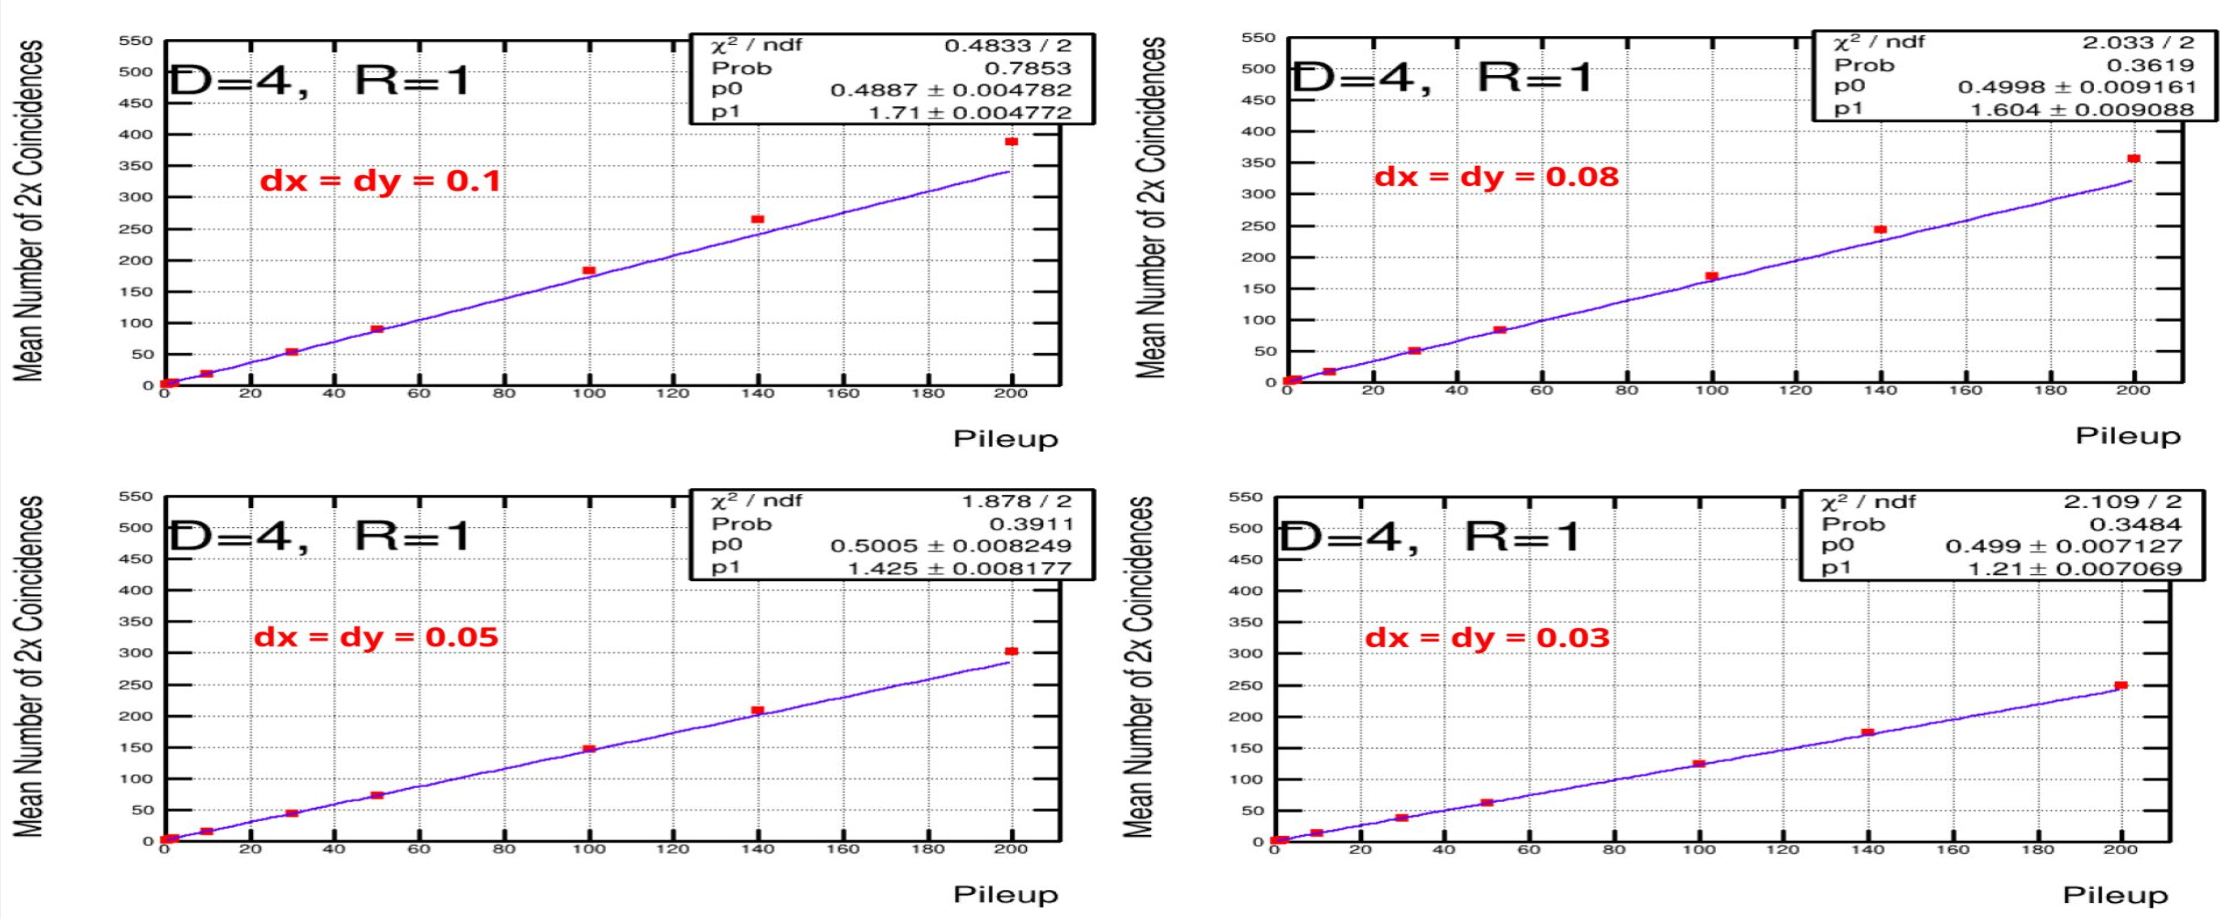
\includegraphics[width=1\textwidth]{ashish_thesis/cut_optimization_twofoldcoin.png}
\caption{%
 Cut optimization for two fold coincidences based on x, y variables to compute coincidence cluster separation.
}
\label{fig:cutopdxdy}
\end{figure}



\begin{figure}[!htp]
\centering
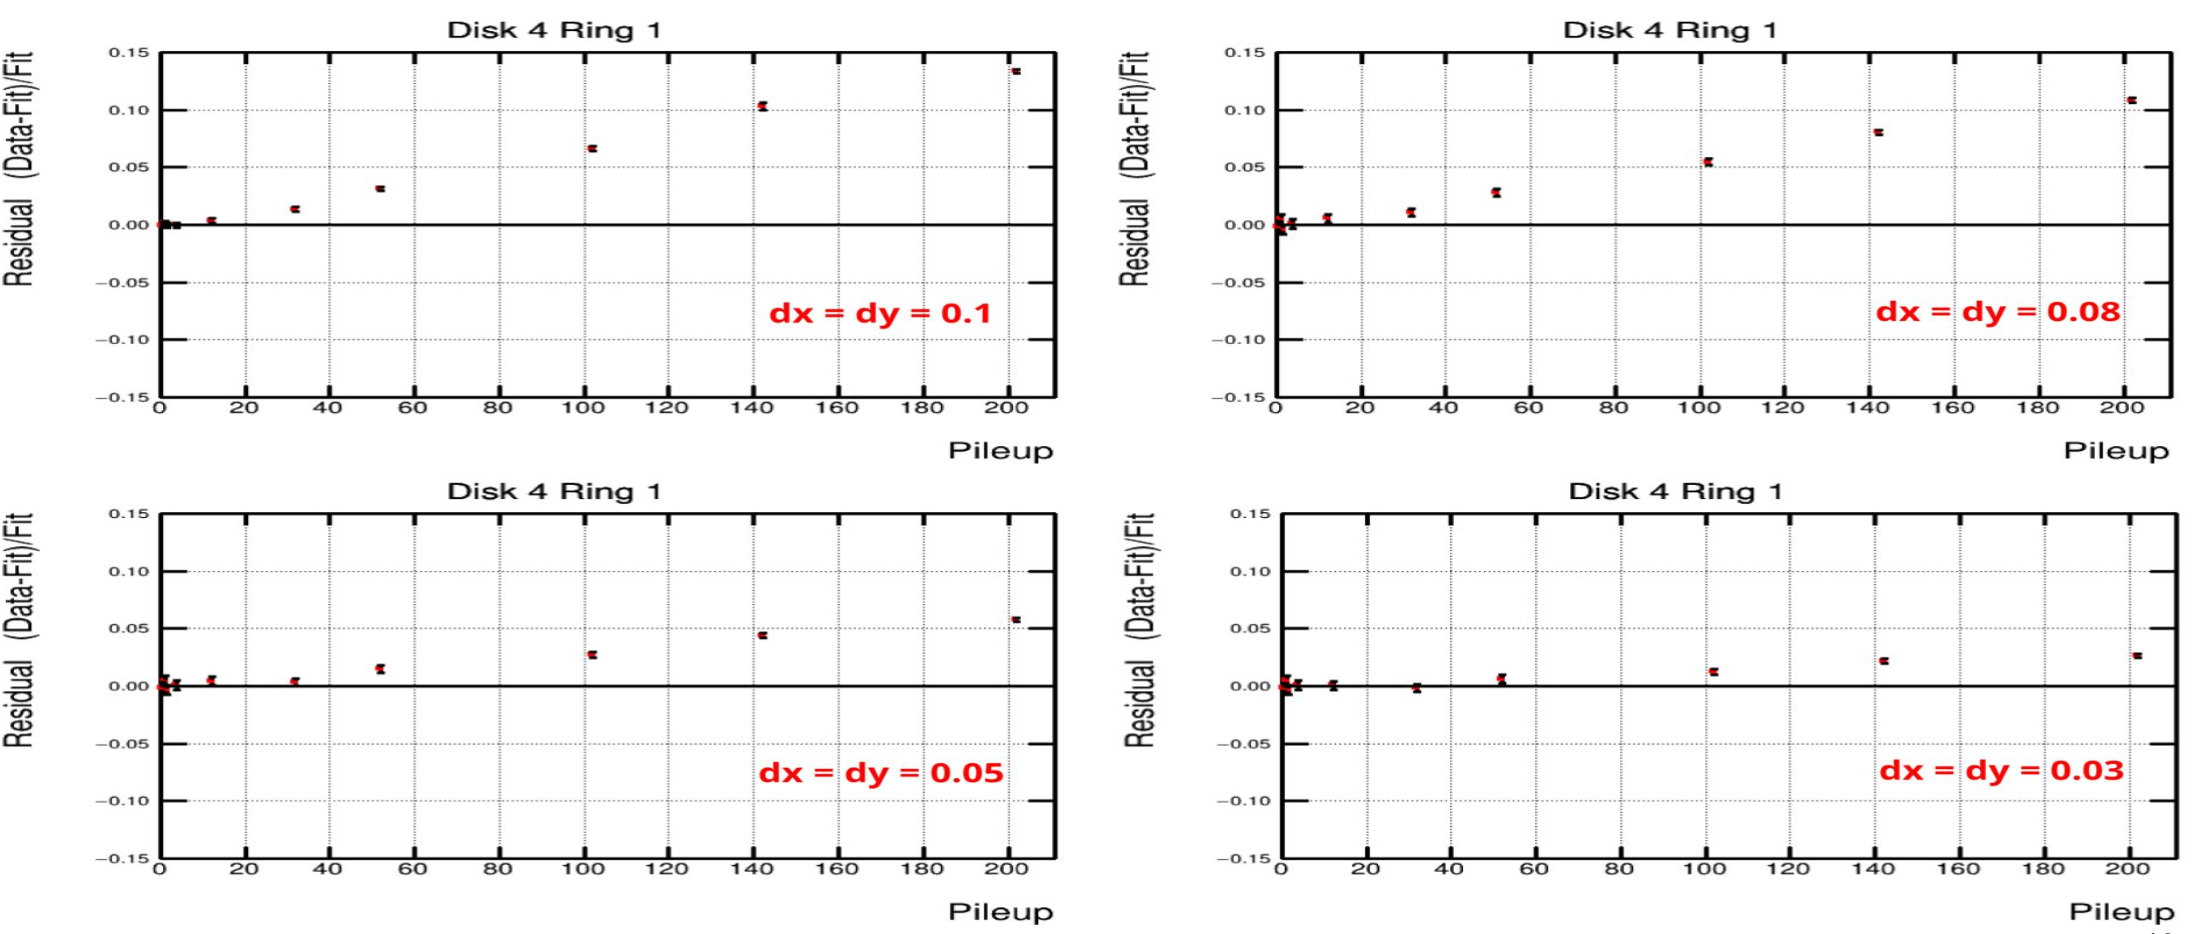
\includegraphics[width=1\textwidth]{ashish_thesis/cut_optimization_residual.png}
\caption{%
  Residual obtained after doing linear fit for different values of dx and dy. Two fold coincidences does not show decrement for high pileup when more stringent selections are applied on dx, dy variables.
}
\label{fig:res_dxdycut}
\end{figure}


\subsection{New algorithm for counting TEPX two fold coincidences}

\subsection{TEPX two fold coincidences in phi}

A new algorithm for luminosity determination based on counting two fold coincidences is proposed that applies selections using dr and $d\phi$ variables to minimize non-linearity for high pileup values as these variables take into account track angle and its curvature. Two fold coincidences are those hits which are created by the module overlap regions between various layers of one TEPX double disk. Two fold coincidences are better way to distinguish between a real hit and random electrical noise. They are more likely to be real hit than random electrical noise. Two fold coincidence in $\phi$ will involve modules overlapping in the same ring in front and back layers of one double disk as shown in top part of Fig. 27 and Fig. 28 while two fold coincidence in r will require modules overlapping between successive rings in the front (L1 $\&$ L2) and back layers (L3 $\&$ L4) of one double disk as shown in bottom part of Fig. 27. Luminosity calculated based on counting coincidences has an advantage over clusters that afterglow effects are tiny in the case of coincidences  %\cite{Collaboration:2706512} \cite{brilsim} \cite{brilsim1}\cite{brilsim2}.

\begin{figure}[!htp]
\centering
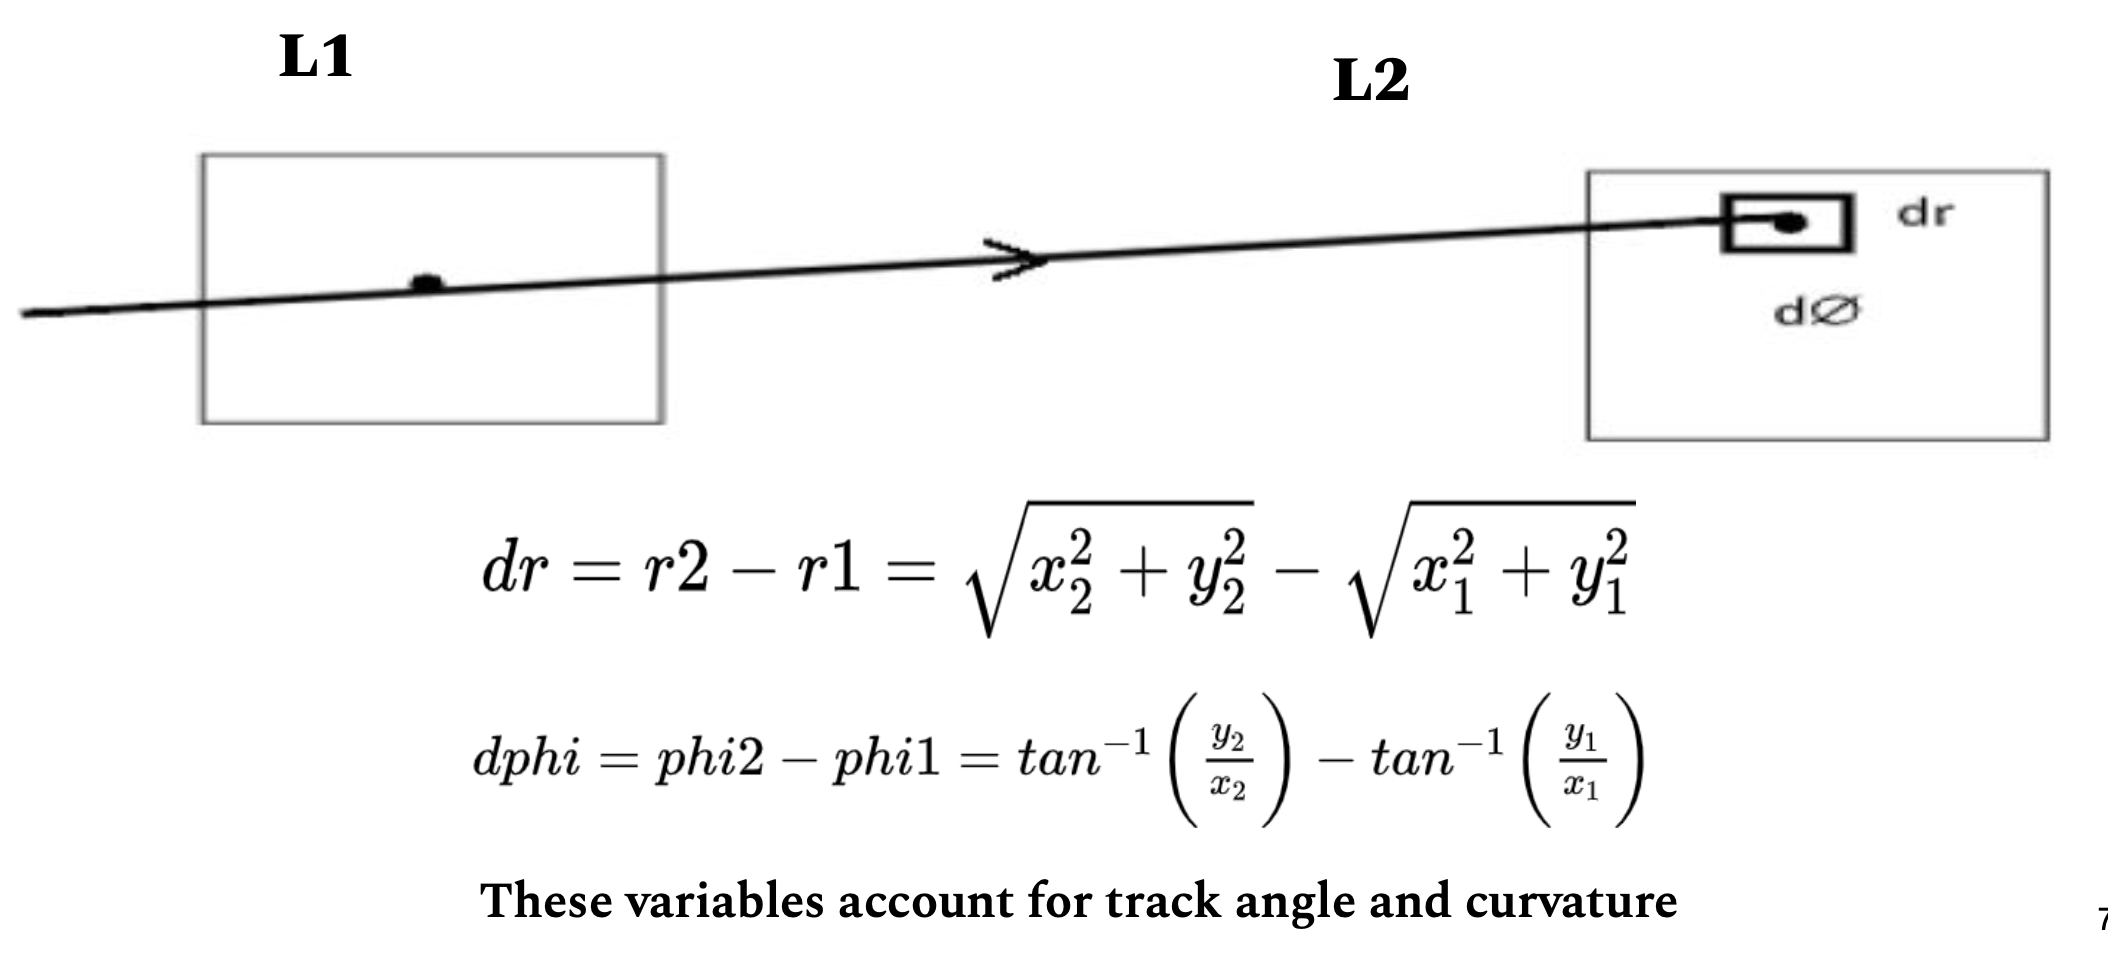
\includegraphics[width=1\textwidth]{ashish_thesis/dr_dphi_variables.png}
\caption{%
  New r, phi variables used to define coincidence clusters. These variables take into account track angle and curvature.
}
\label{fig:drdphi_diagram}
\end{figure}


\begin{figure}[!htp]
\centering
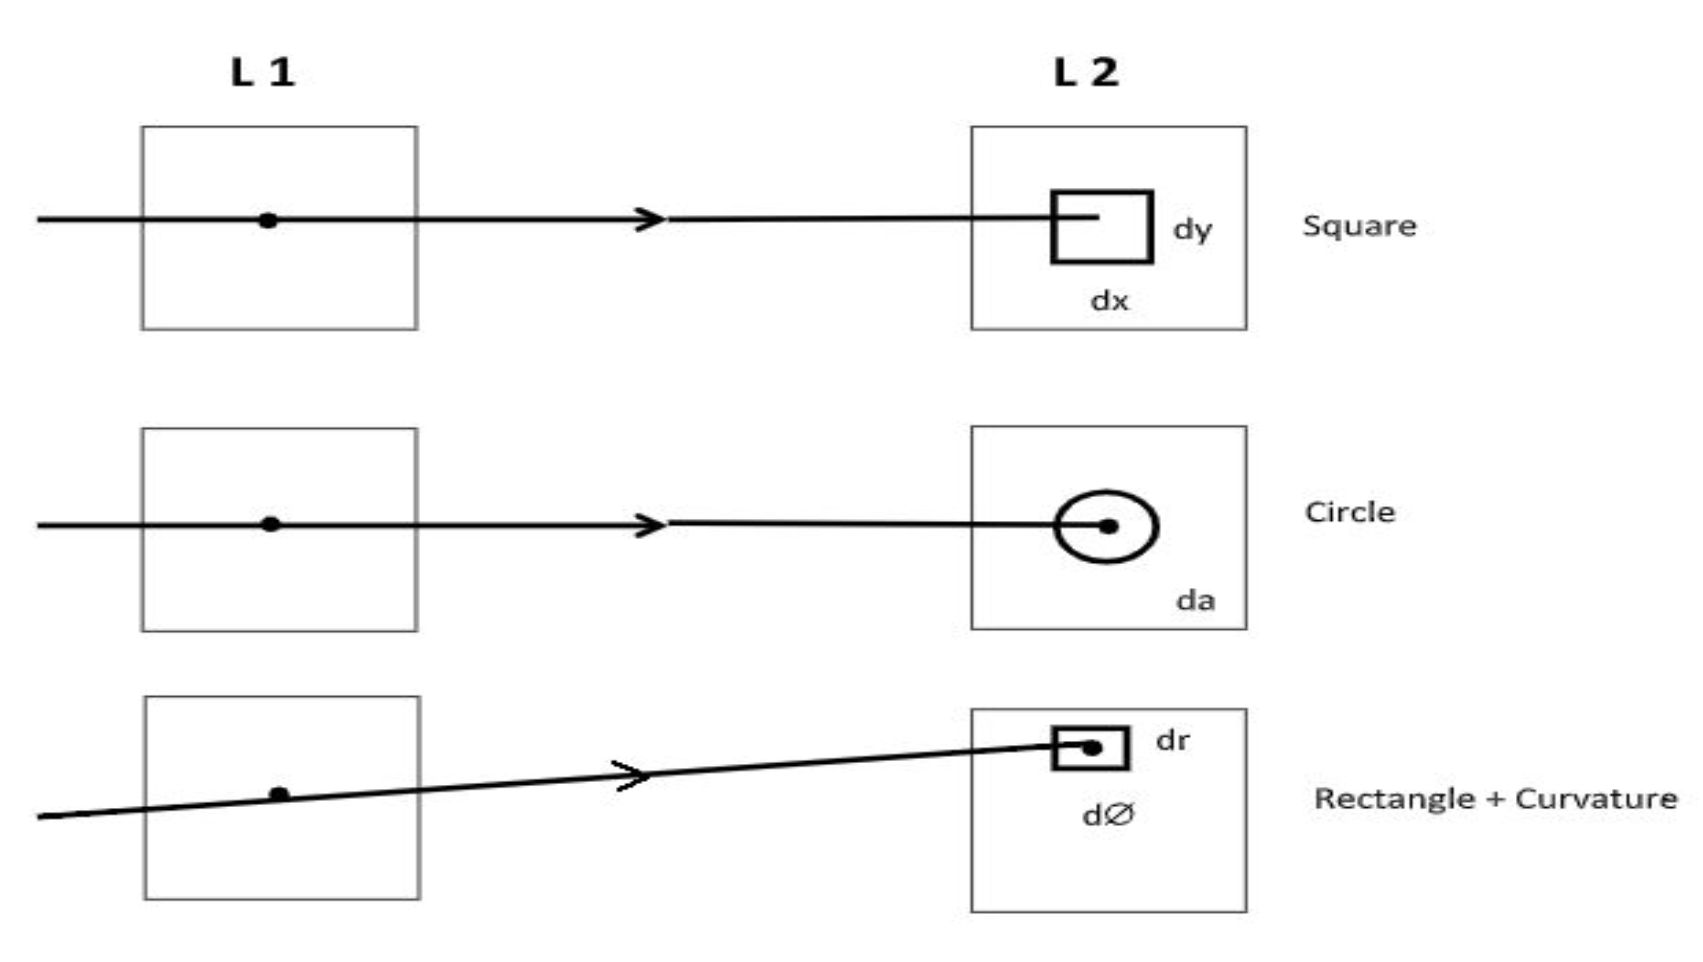
\includegraphics[width=1\textwidth]{ashish_thesis/new_variables.png}
\caption{%
   Possible new variable to replace x, y variable for defining coincidence clusters.
}
\label{fig:newvar}
\end{figure}


\begin{figure}[!htp]
\centering
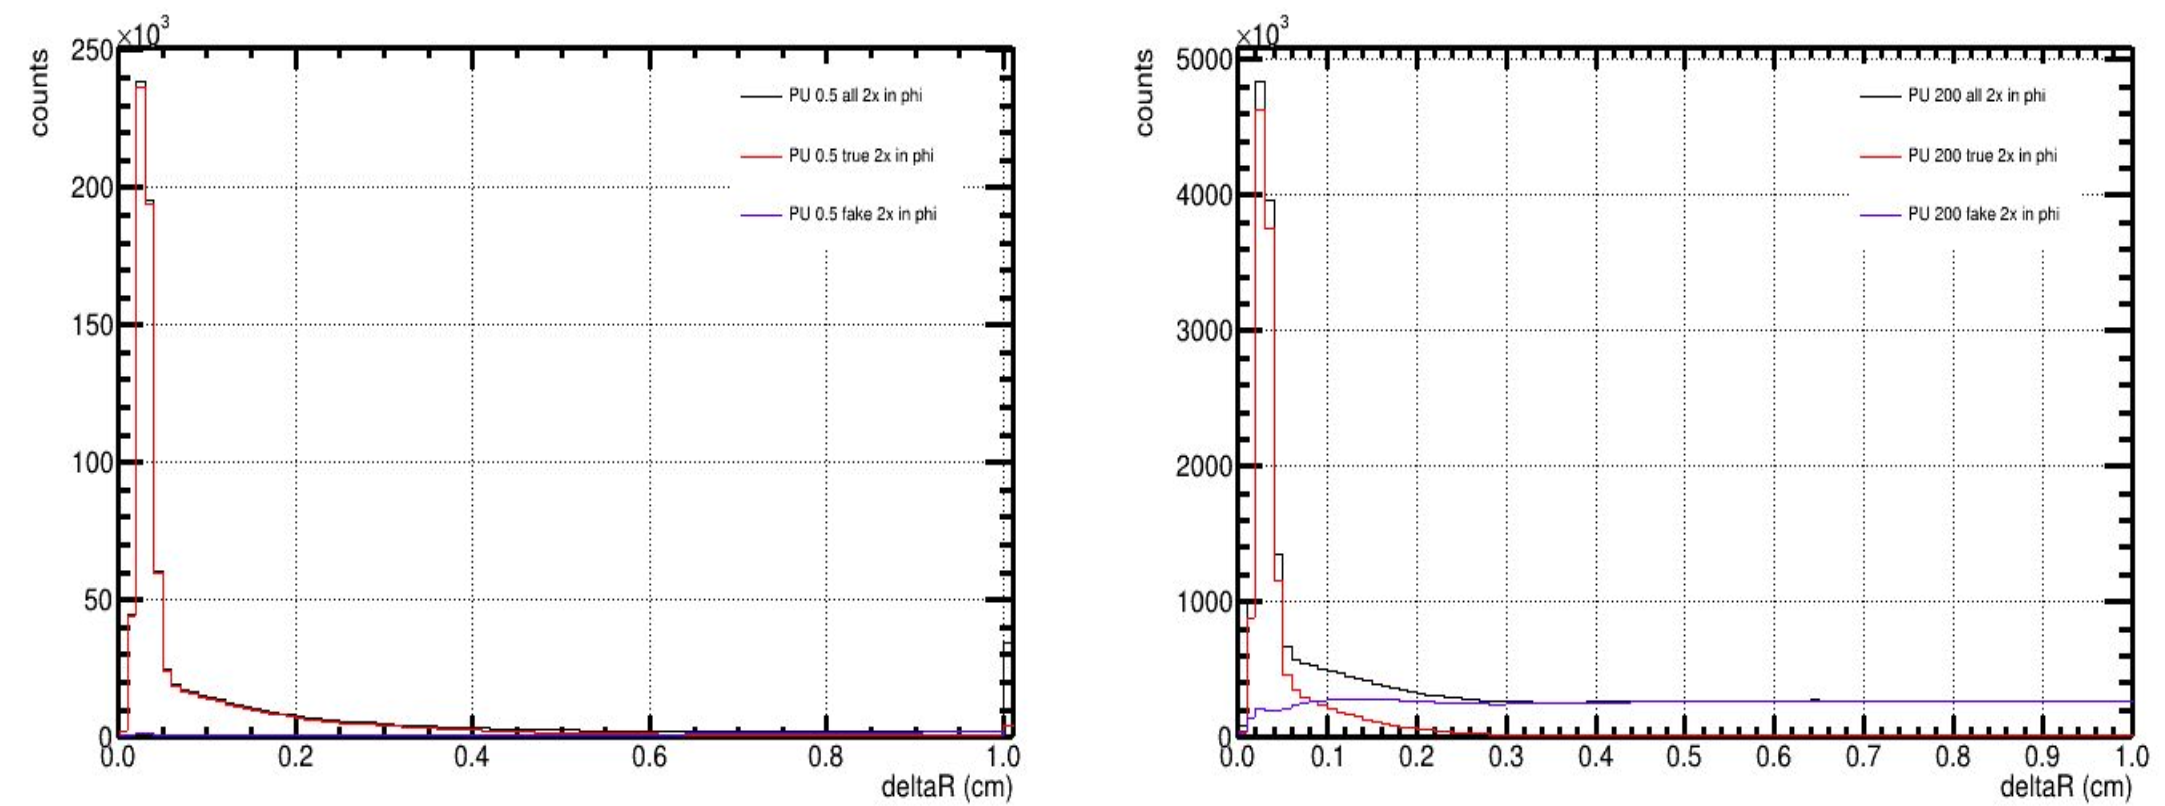
\includegraphics[width=1\textwidth]{ashish_thesis/deltaR.png}
\caption{%
 dR
}
\label{fig:dR}
\end{figure}


\begin{figure}[!htp]
\centering
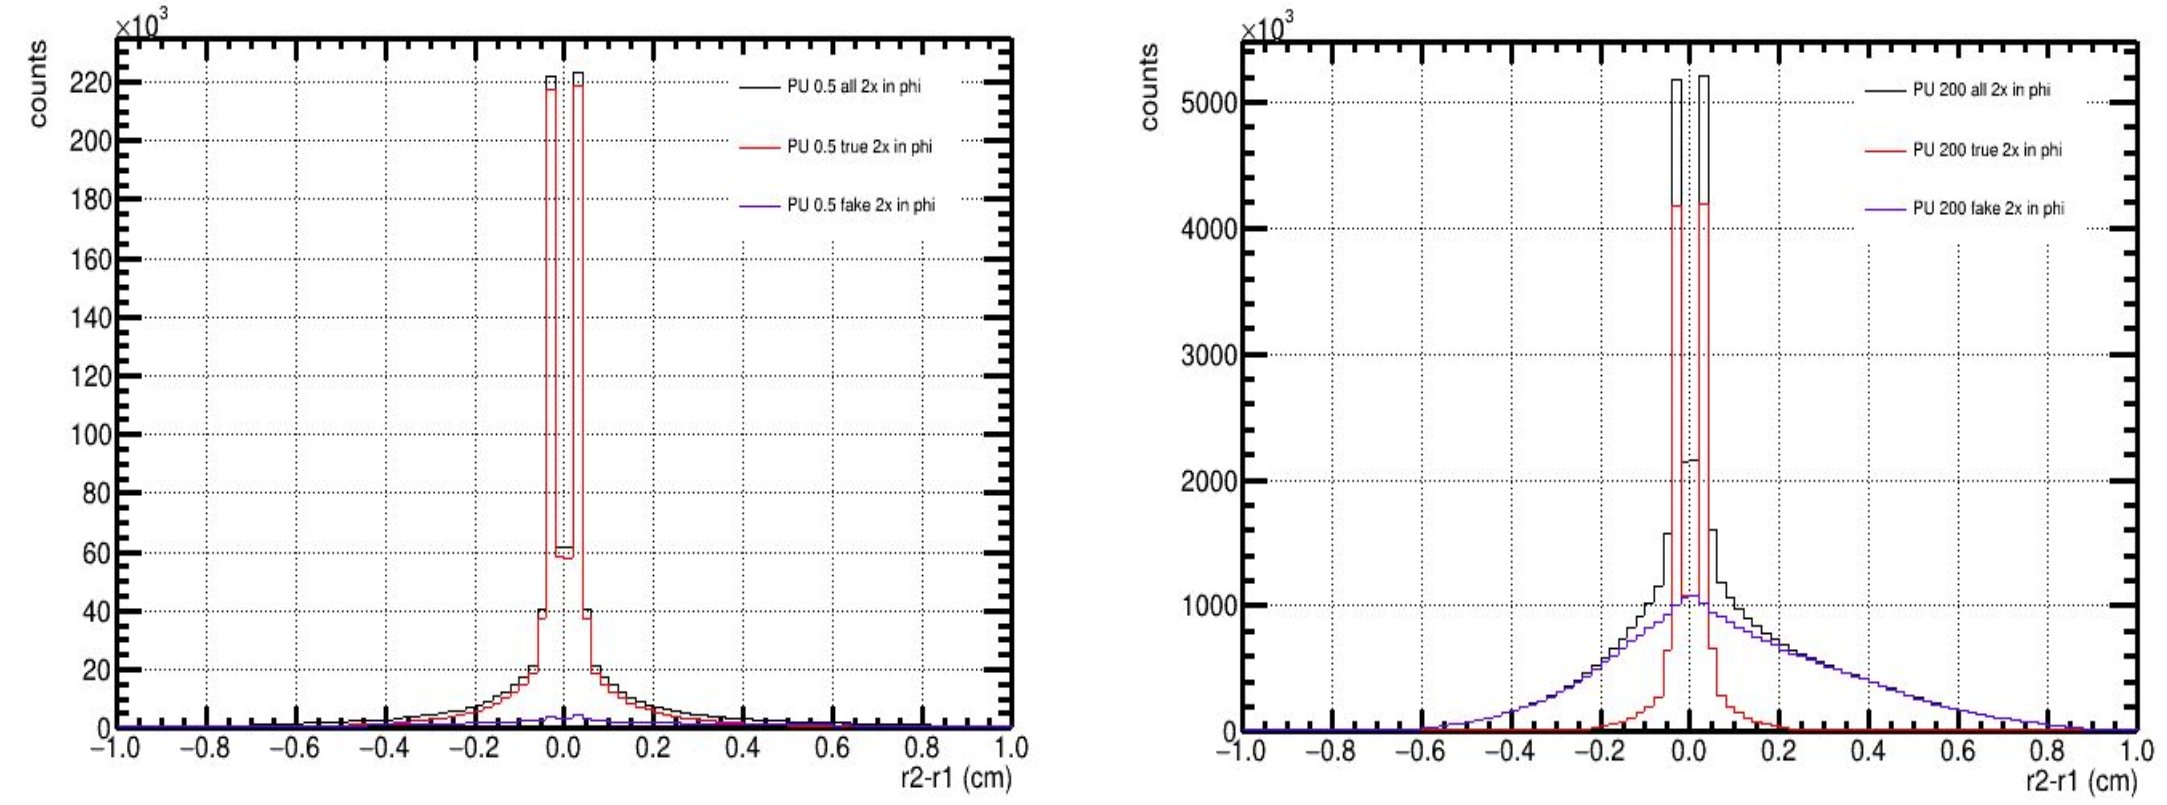
\includegraphics[width=1\textwidth]{ashish_thesis/delta_r.png}
\caption{%
  dr
}
\label{fig:dr}
\end{figure}


\begin{figure}[!htp]
\centering
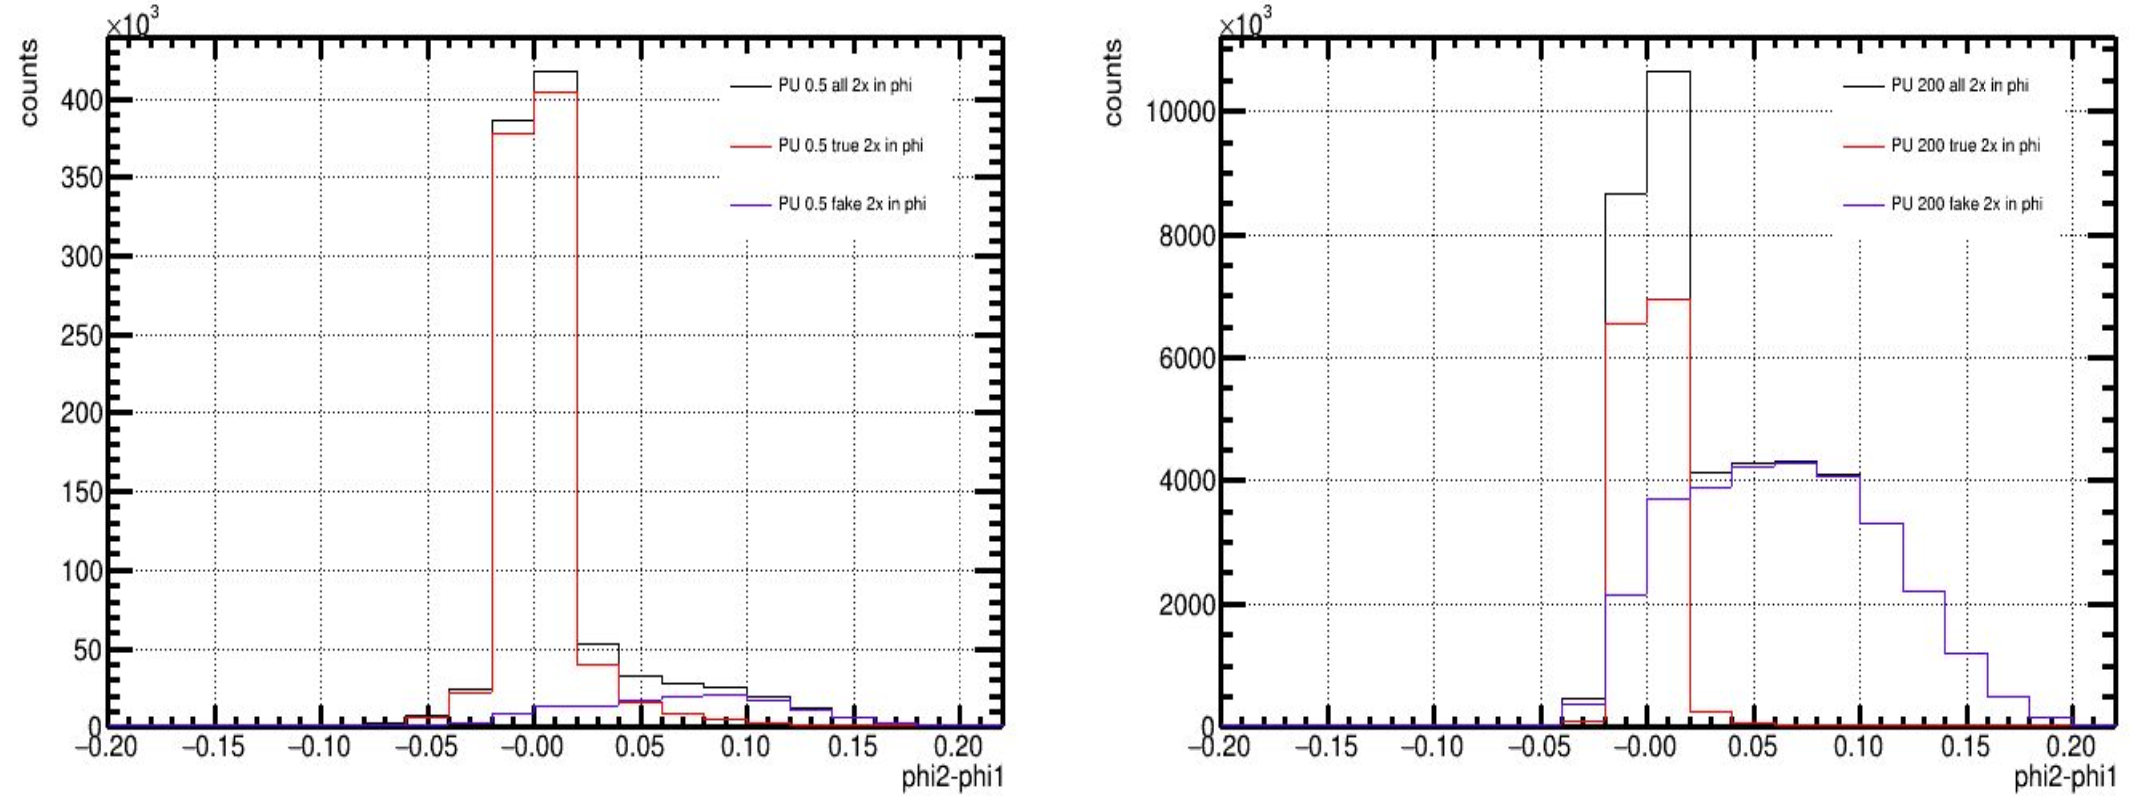
\includegraphics[width=1\textwidth]{ashish_thesis/dphi.png}
\caption{%
 dphi 
}
\label{fig:dphi}
\end{figure}


\begin{figure}[!htp]
\centering
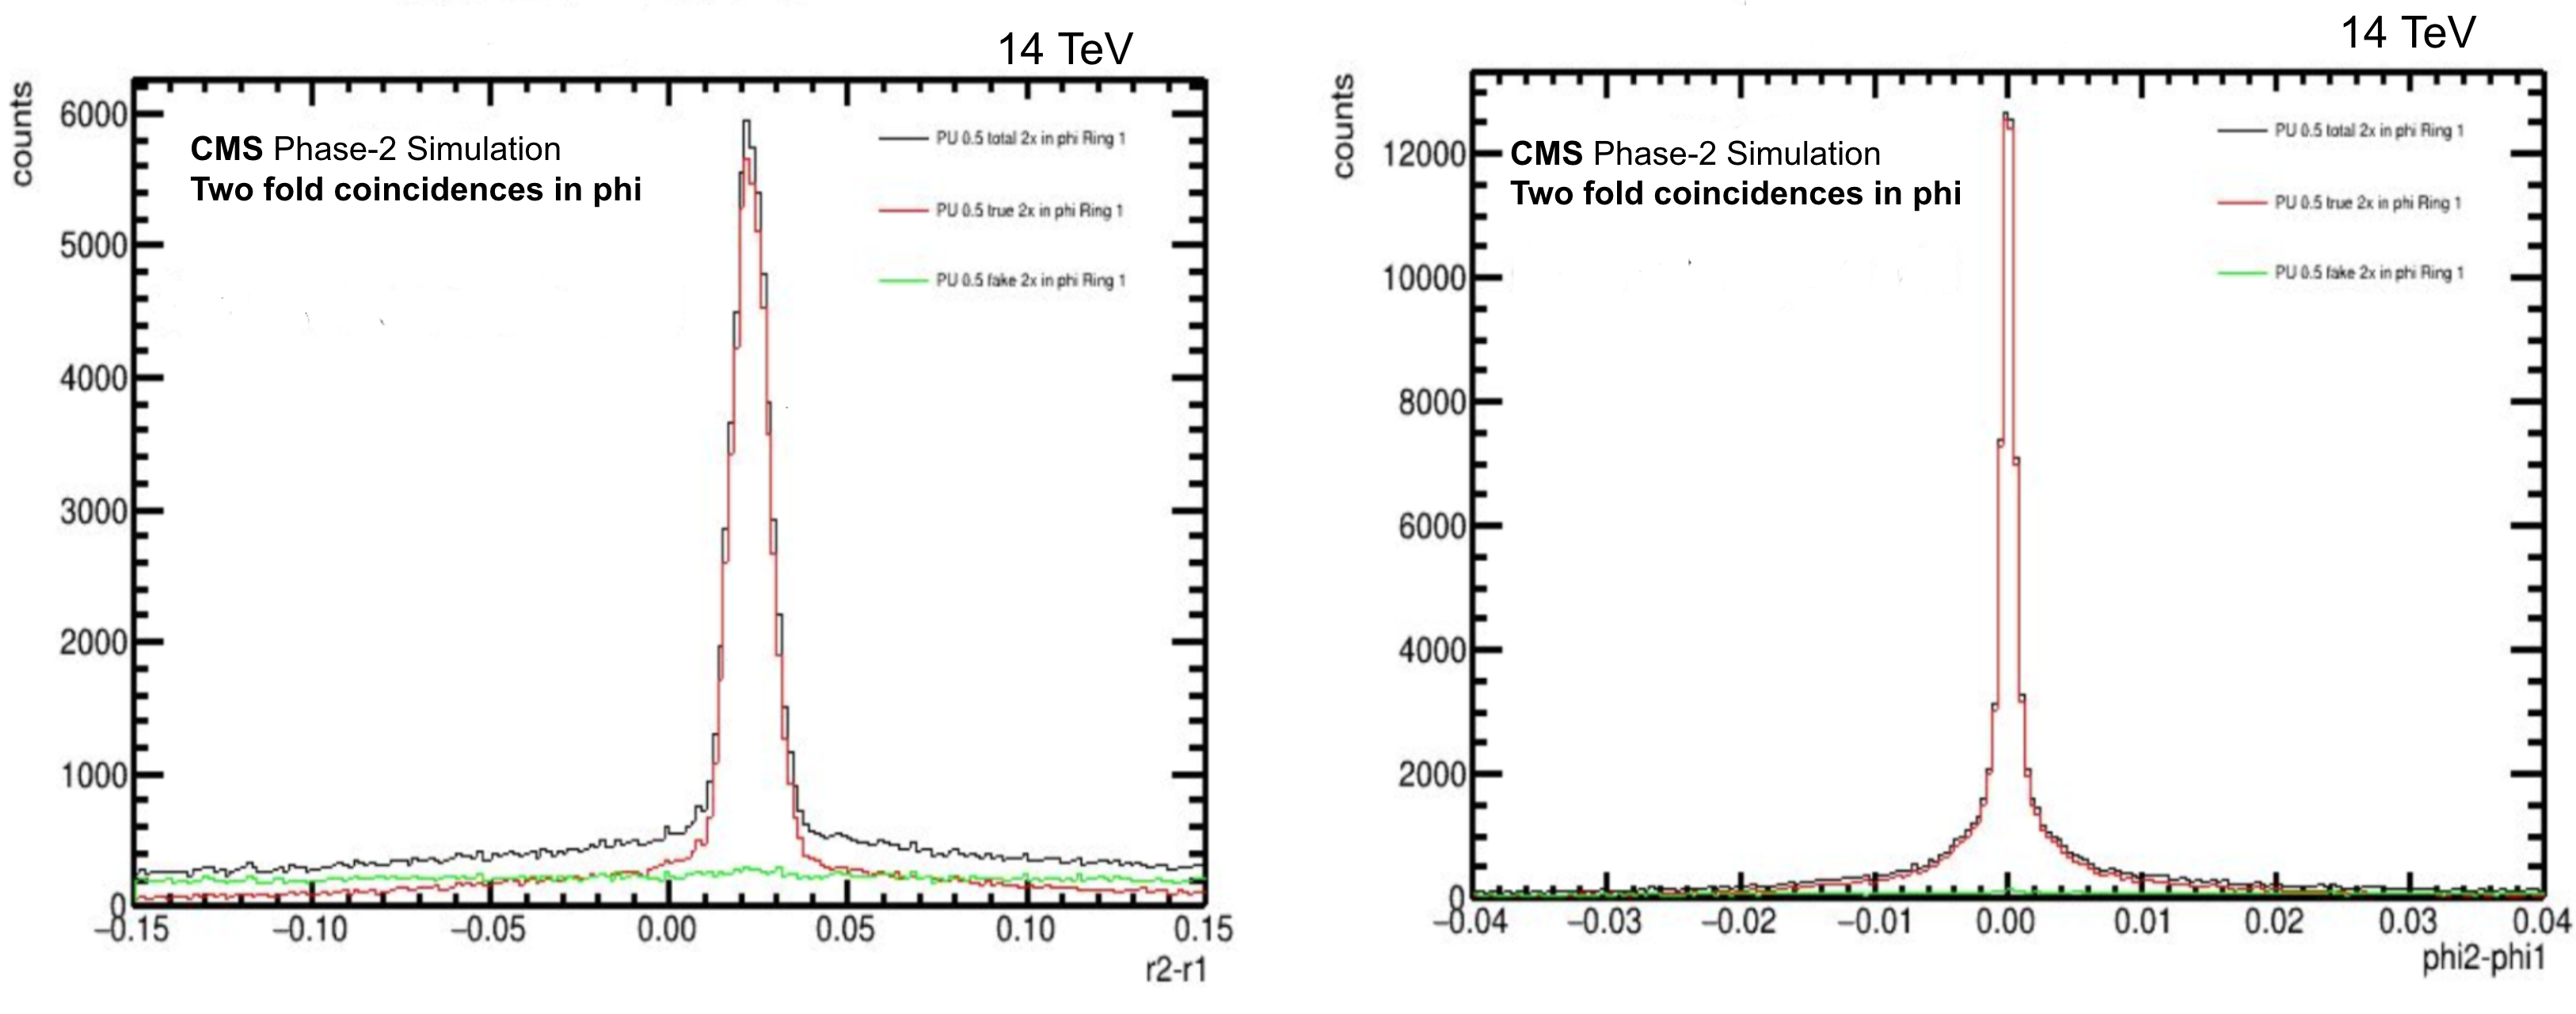
\includegraphics[width=1\textwidth]{ashish_thesis/D4R1_S2_drdphi_cut.png}
\caption{%
  Distribution of cluster count as a function of dr and dphi variables for pileup 0.5 for disk 4 Ring 1 (+Z). Appropriate selection on dr, dphi are used to minimize fake two fold coincidence clusters.
}
\label{fig:cluster_dr_dphi_dist}
\end{figure}



\begin{figure}[!htp]
\centering
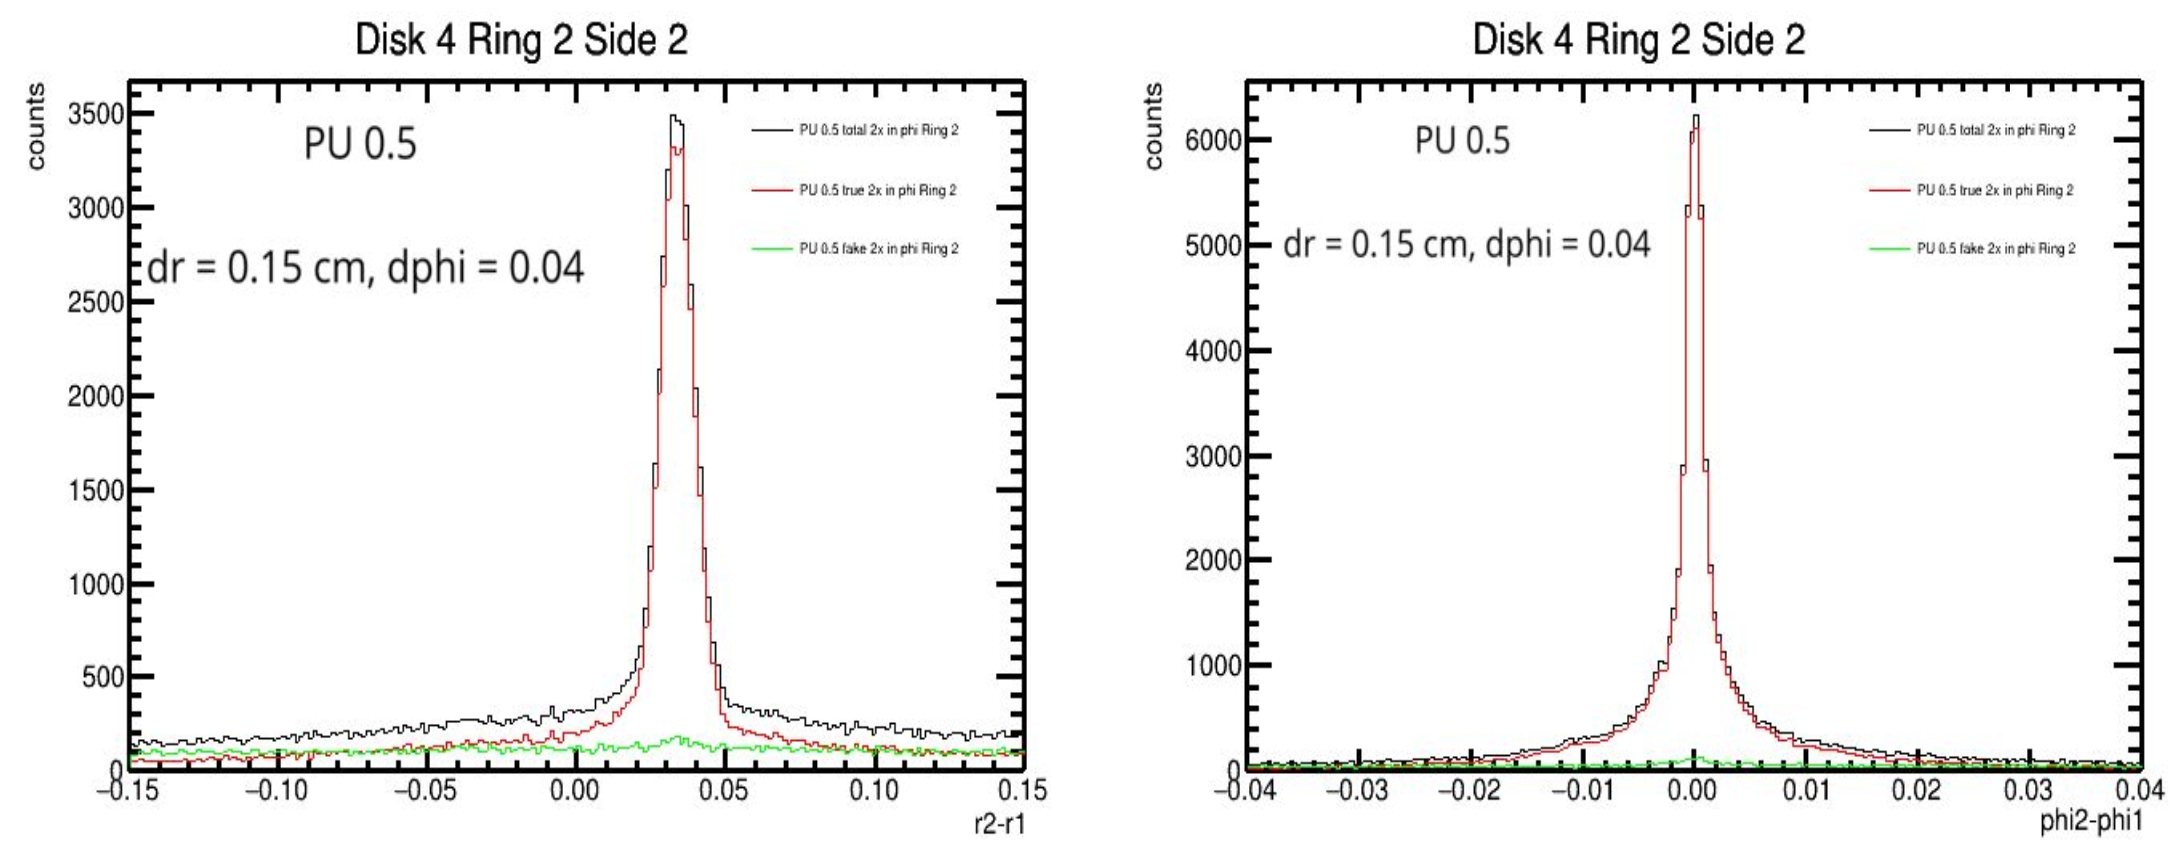
\includegraphics[width=1\textwidth]{ashish_thesis/D4R2_S2_drdphicut.png}
\caption{%
   Distribution of cluster count as a function of dr and dphi variables for pileup 0.5 for disk 4 Ring 2 (+Z). Appropriate selection on dr, dphi are used to minimize fake two fold coincidence clusters.
}
\label{fig:cluster_ring}
\end{figure}


\begin{figure}[!htp]
\centering
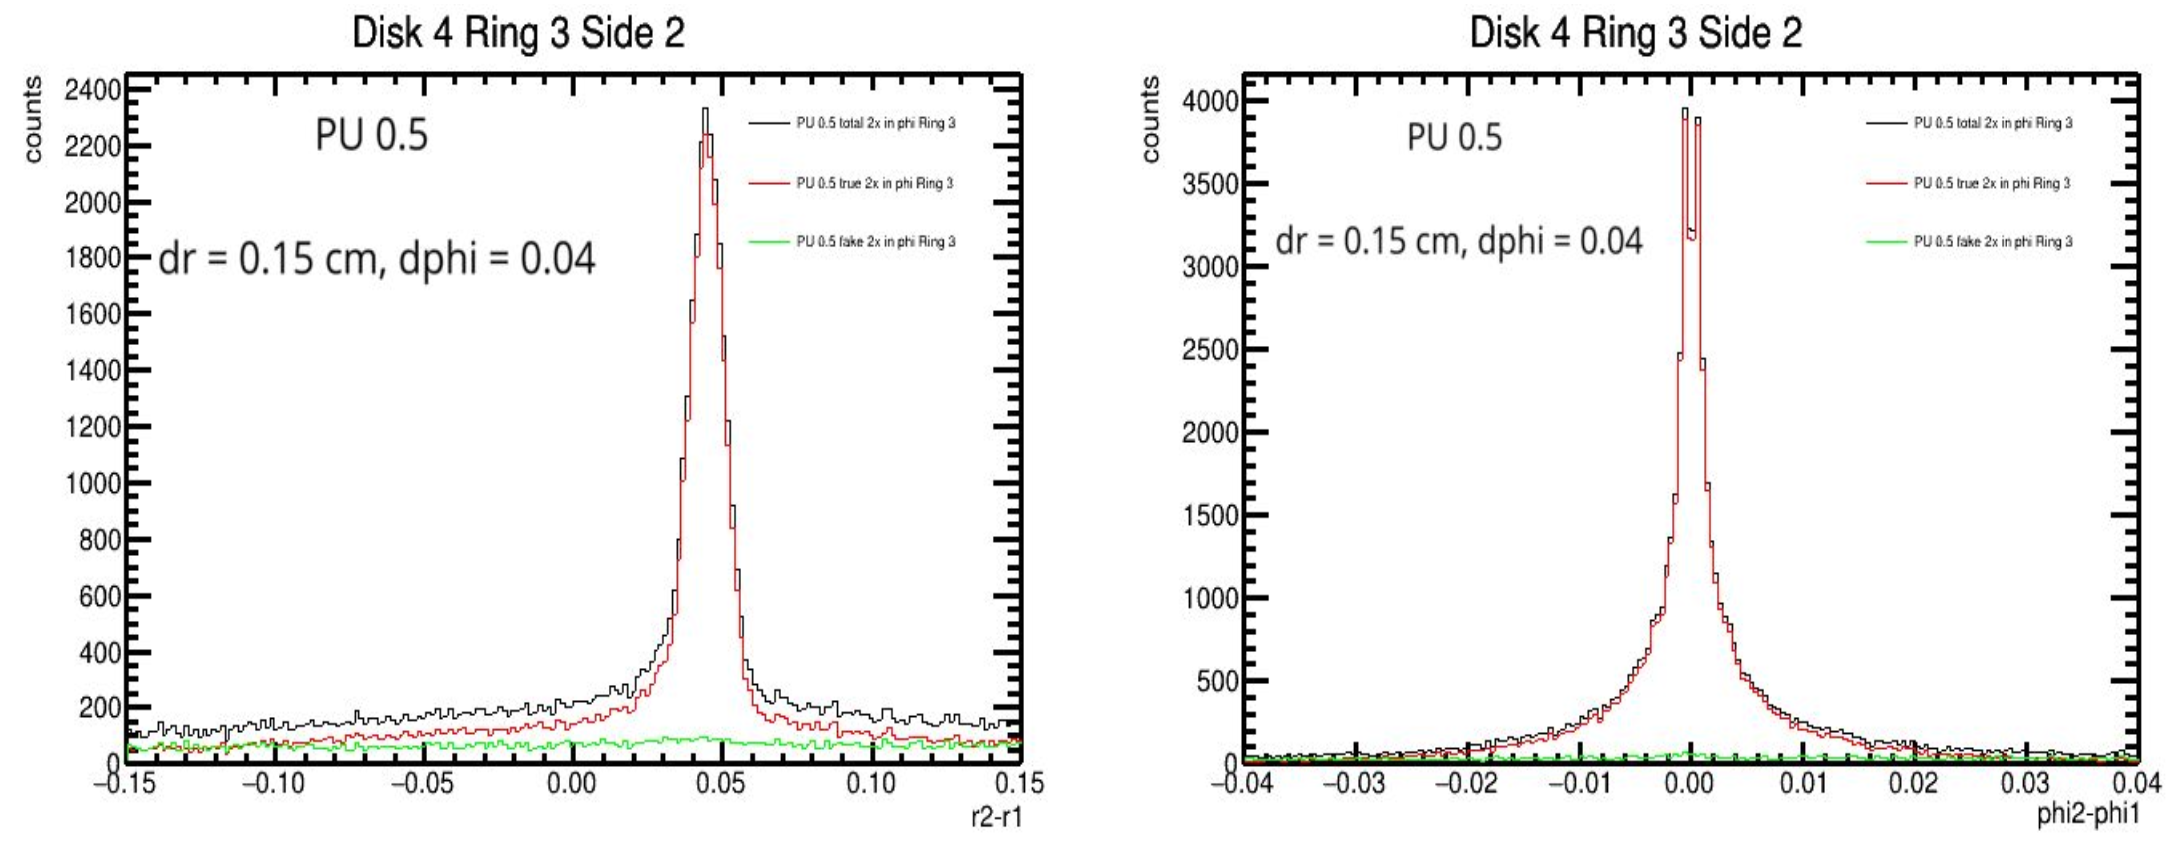
\includegraphics[width=1\textwidth]{ashish_thesis/D4R3_S2_drdphi_cut.png}
\caption{%
  Distribution of cluster count as a function of dr and dphi variables for pileup 0.5 for disk 4 Ring 3 (+Z). Appropriate selection on dr, dphi are used to minimize fake two fold coincidence clusters.
}
\label{fig:cluster_ring}
\end{figure}


\begin{figure}[!htp]
\centering
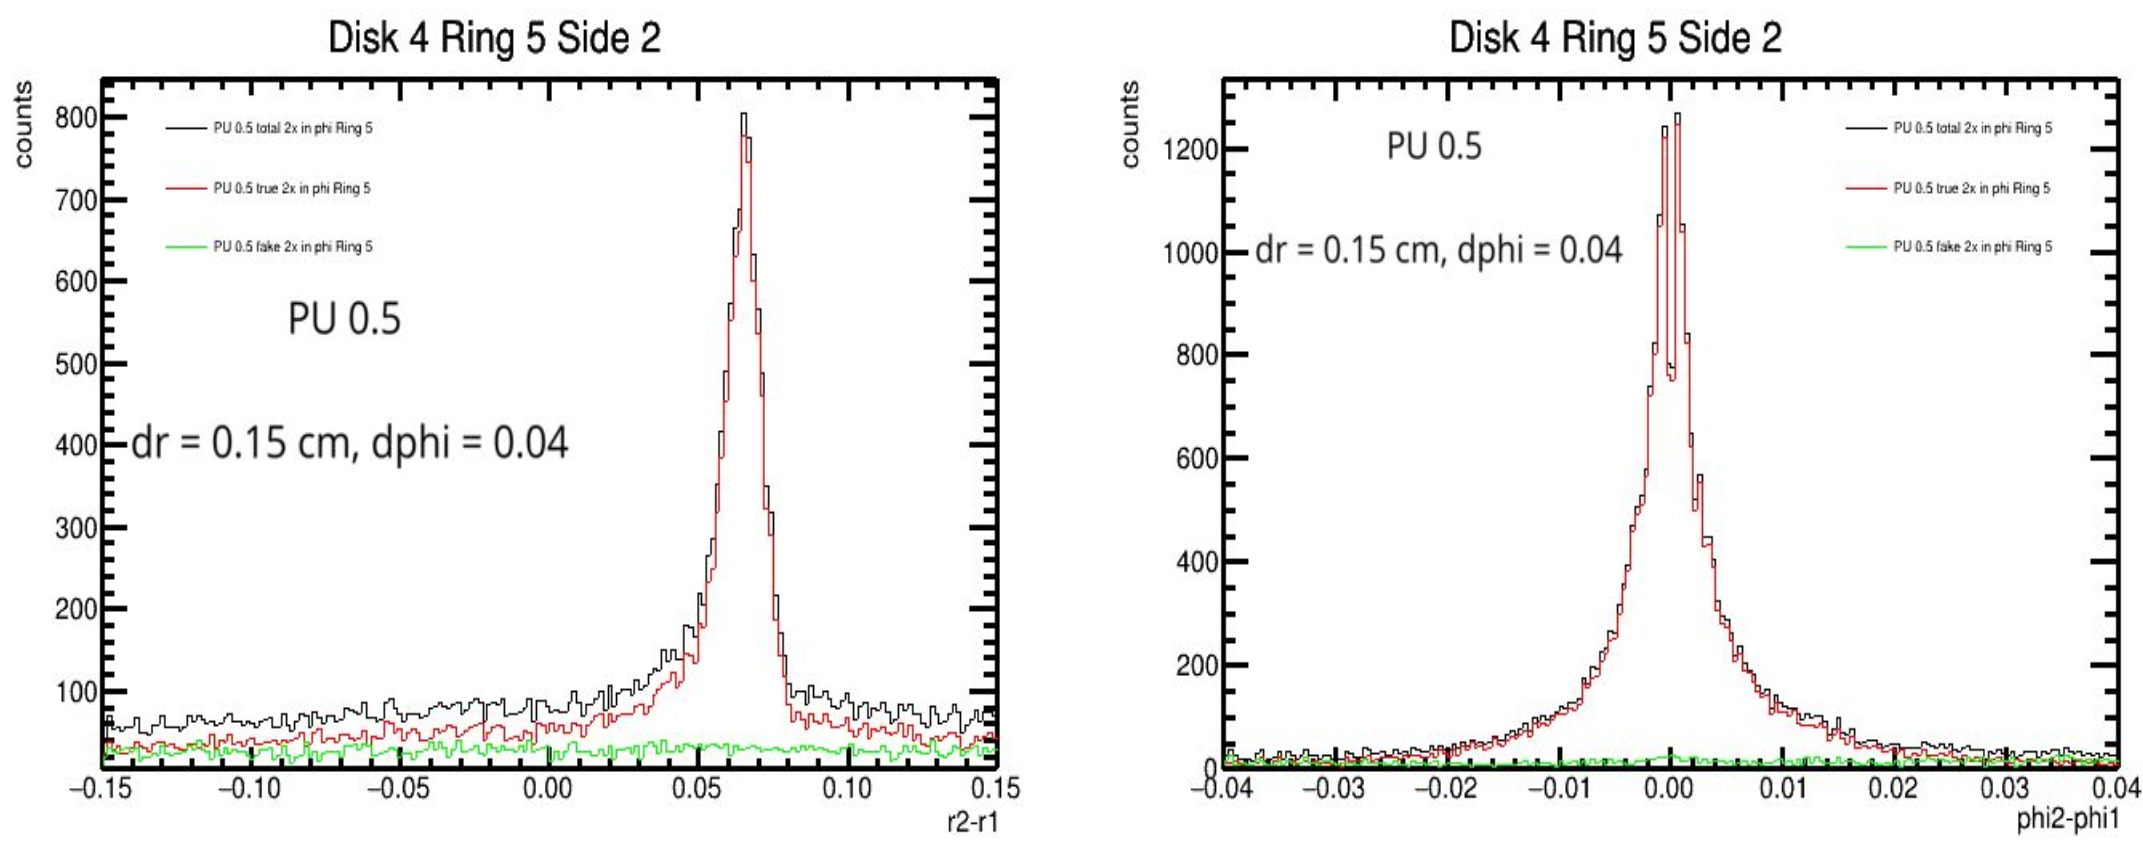
\includegraphics[width=1\textwidth]{ashish_thesis/D4R5_drdphicut.png}
\caption{%
  Distribution of cluster count as a function of dr and dphi variables for pileup 0.5 for disk 4 Ring 5 (+Z). Appropriate selection on dr, dphi are used to minimize fake two fold coincidence clusters.
}
\label{fig:cluster_ring}
\end{figure}


\begin{figure}[!htp]
\centering
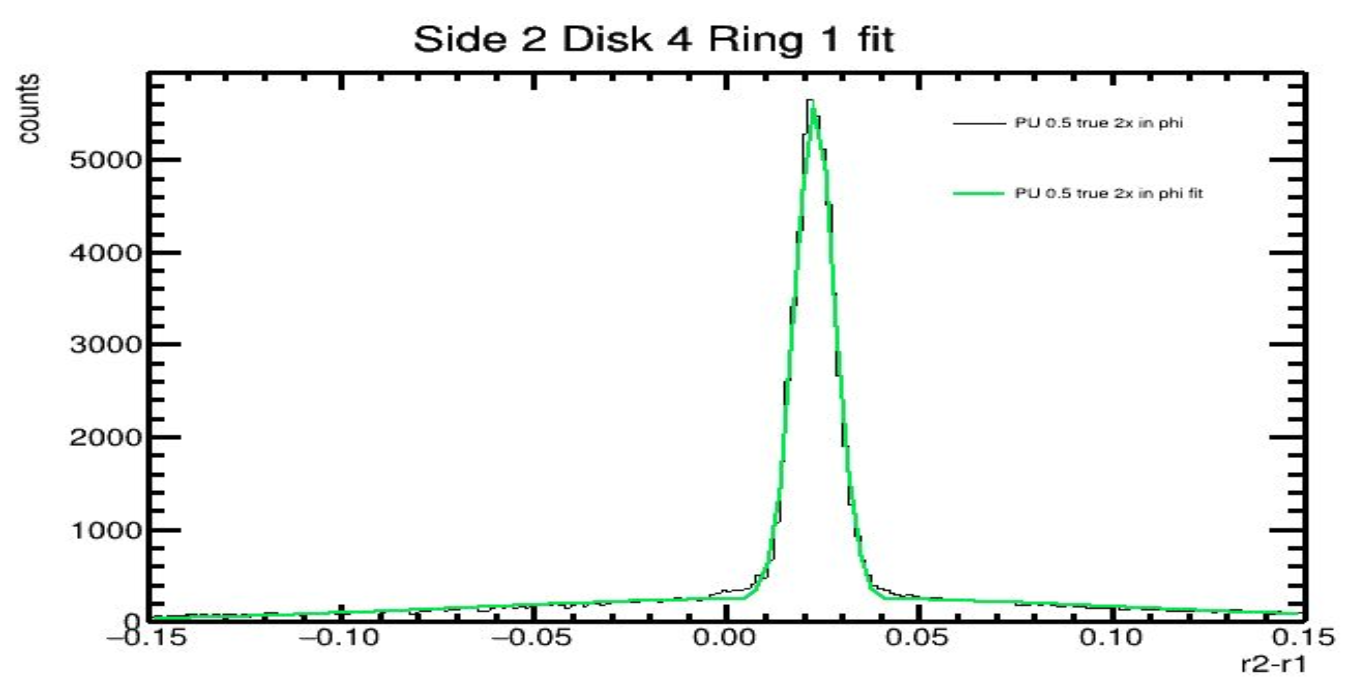
\includegraphics[width=1\textwidth]{ashish_thesis/D4R1S2_fit.png}
\caption{%
   Example fit using single gaussian function of cluster count as a function of dr variable for Disk 4 Ring 1 (+Z).
}
\label{fig:cluster_ring}
\end{figure}


\begin{figure}[!htp]
\centering
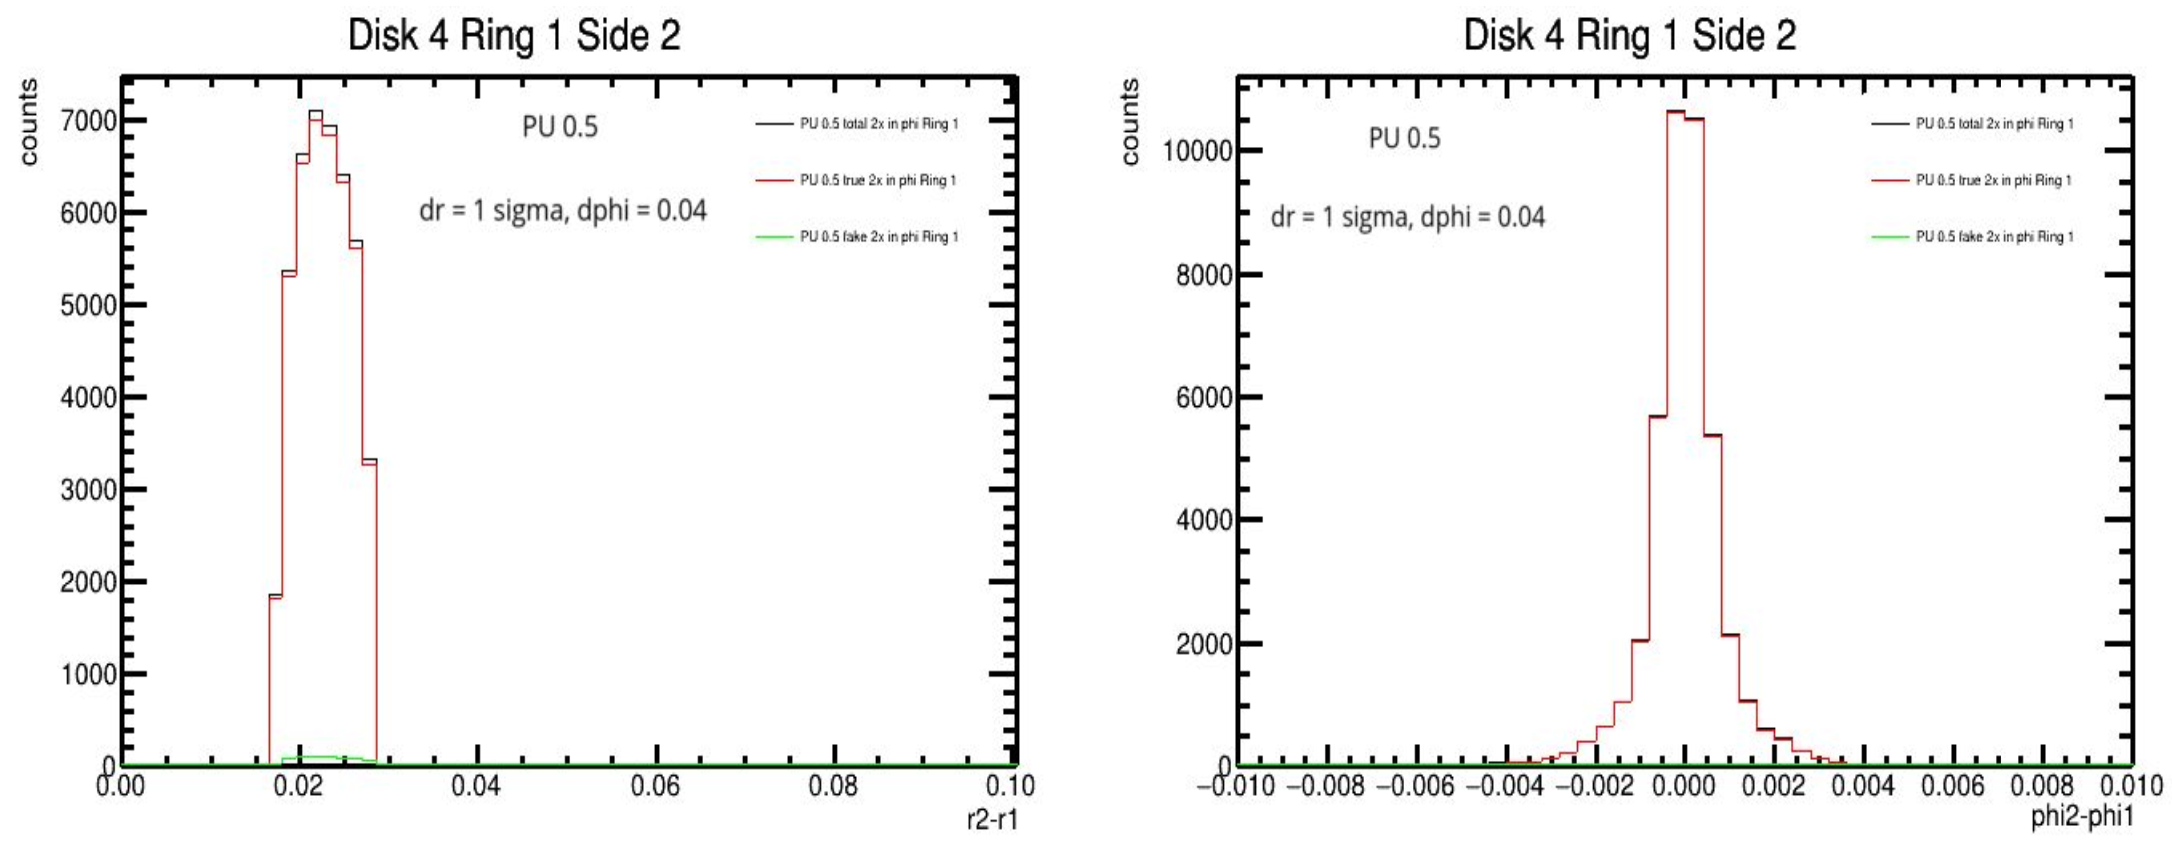
\includegraphics[width=1\textwidth]{ashish_thesis/D4R1S2_dr_dphi_cut.png}
\caption{%
 Distribution of cluster count as a function of dr and dphi variables for pileup 0.5 for disk 4 Ring 1 (+Z). 1 sigma selection on dr and dphi equal to 0.04 are used to minimize fake two fold coincidence clusters.
}
\label{fig:cluster_ring}
\end{figure}



\begin{figure}[!htp]
\centering
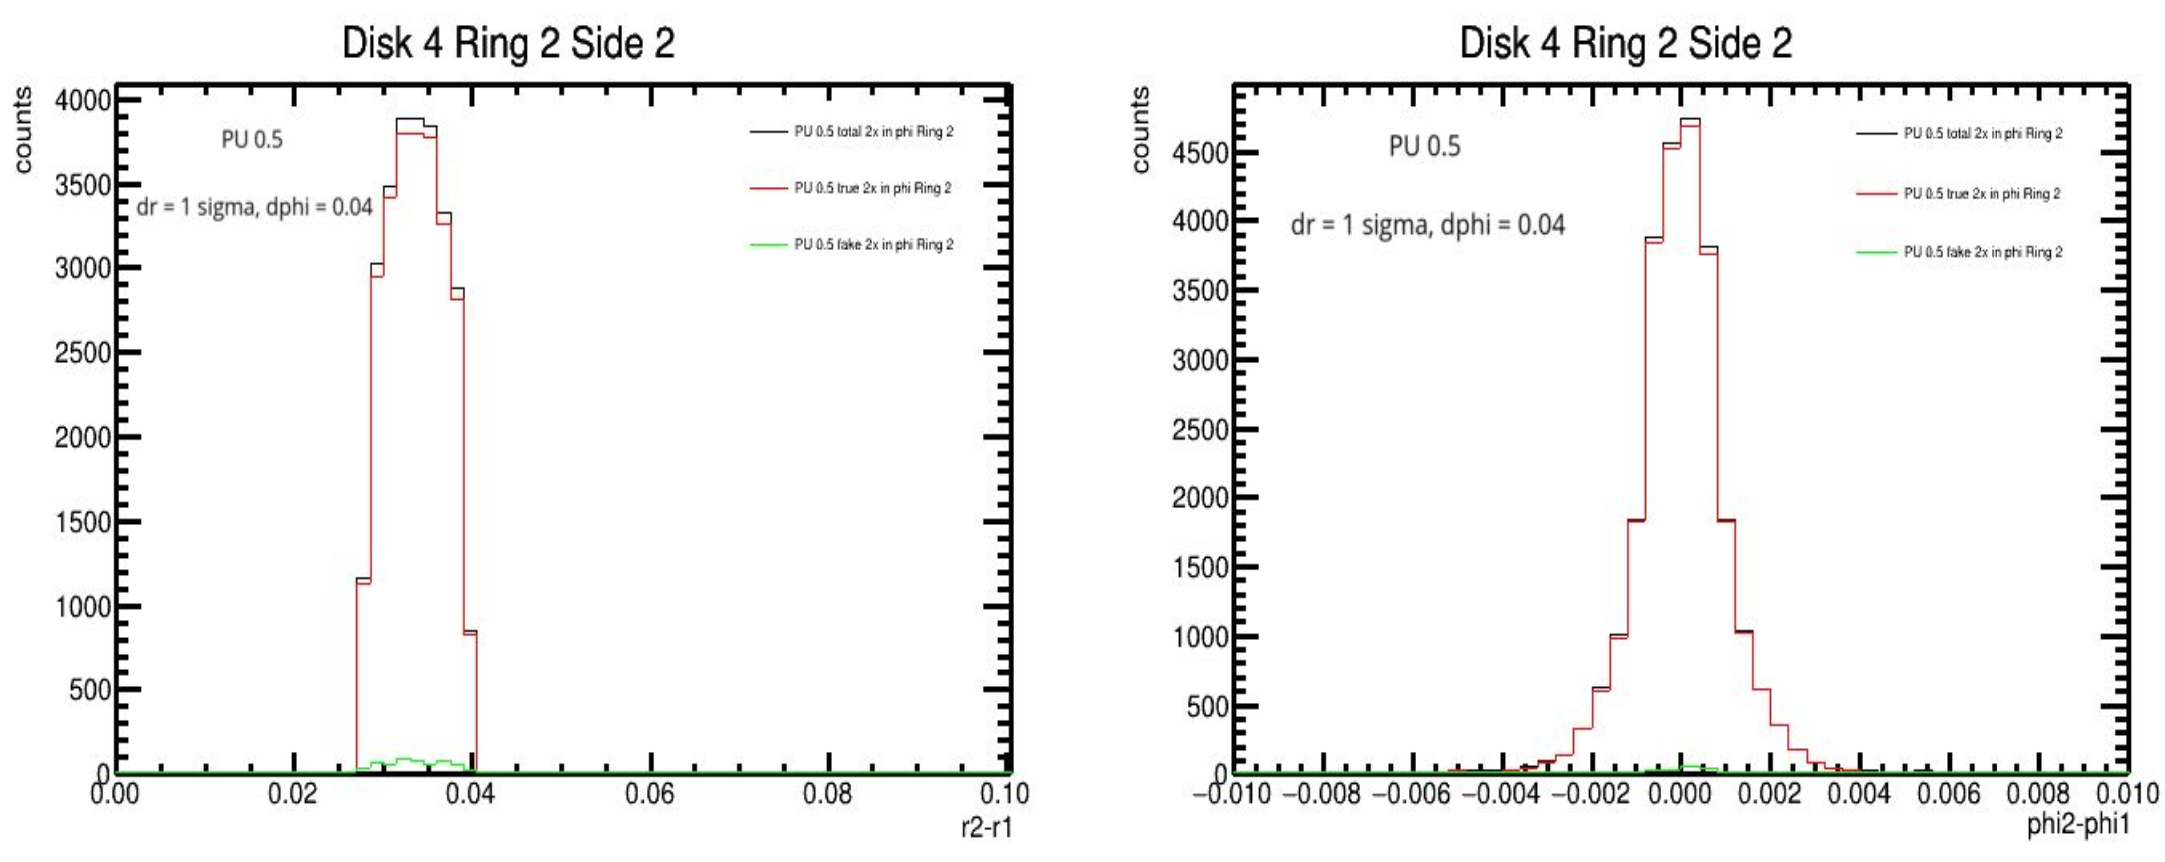
\includegraphics[width=1\textwidth]{ashish_thesis/D4R2S2_dr_dphi_cut.png}
\caption{%
   Distribution of cluster count as a function of dr and dphi variables for pileup 0.5 for disk 4 Ring 2 (+Z). 1 sigma selection on dr and dphi equal to 0.04 are used to minimize fake two fold coincidence clusters.
}
\label{fig:cluster_ring}
\end{figure}


\begin{figure}[!htp]
\centering
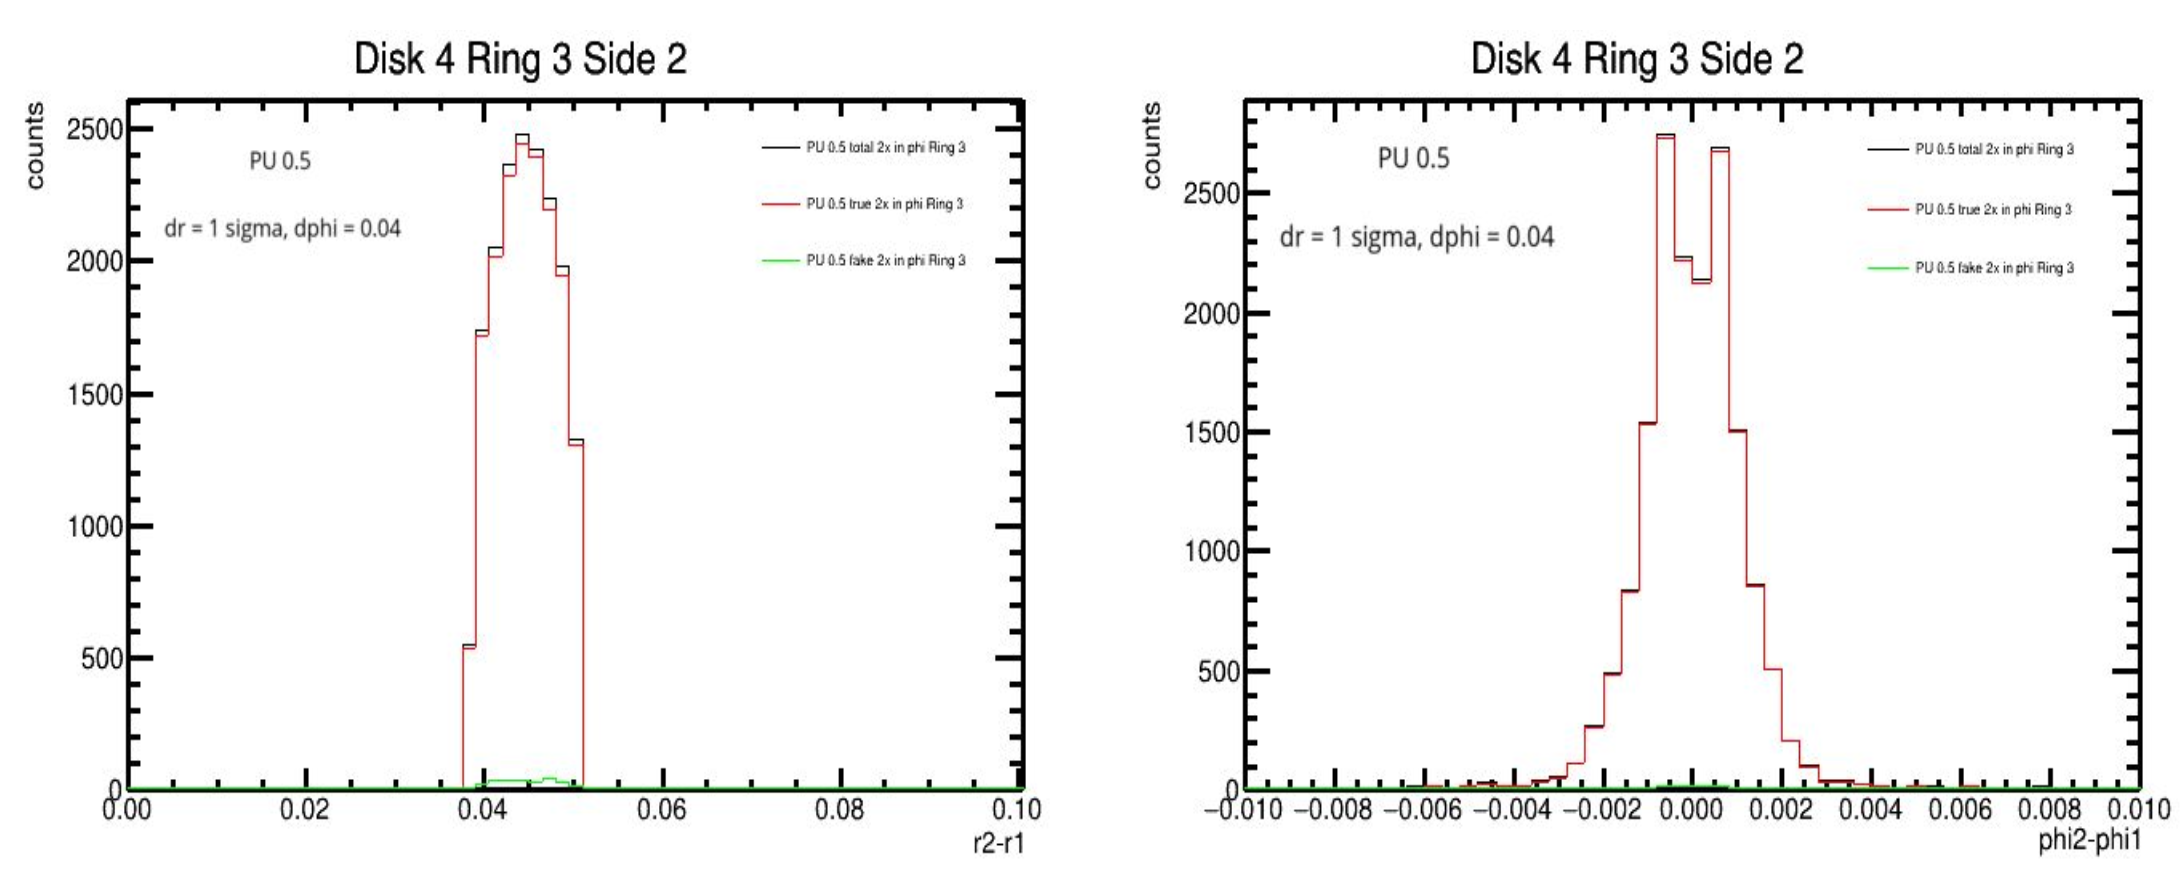
\includegraphics[width=1\textwidth]{ashish_thesis/D4R3S2_dr_dphi_cut.png}
\caption{%
    Distribution of cluster count as a function of dr and dphi variables for pileup 0.5 for disk 4 Ring 3 (+Z). 1 sigma selection on dr and dphi equal to 0.04 are used to minimize fake two fold coincidence clusters.
}
\label{fig:cluster_ring}
\end{figure}



\begin{figure}[!htp]
\centering
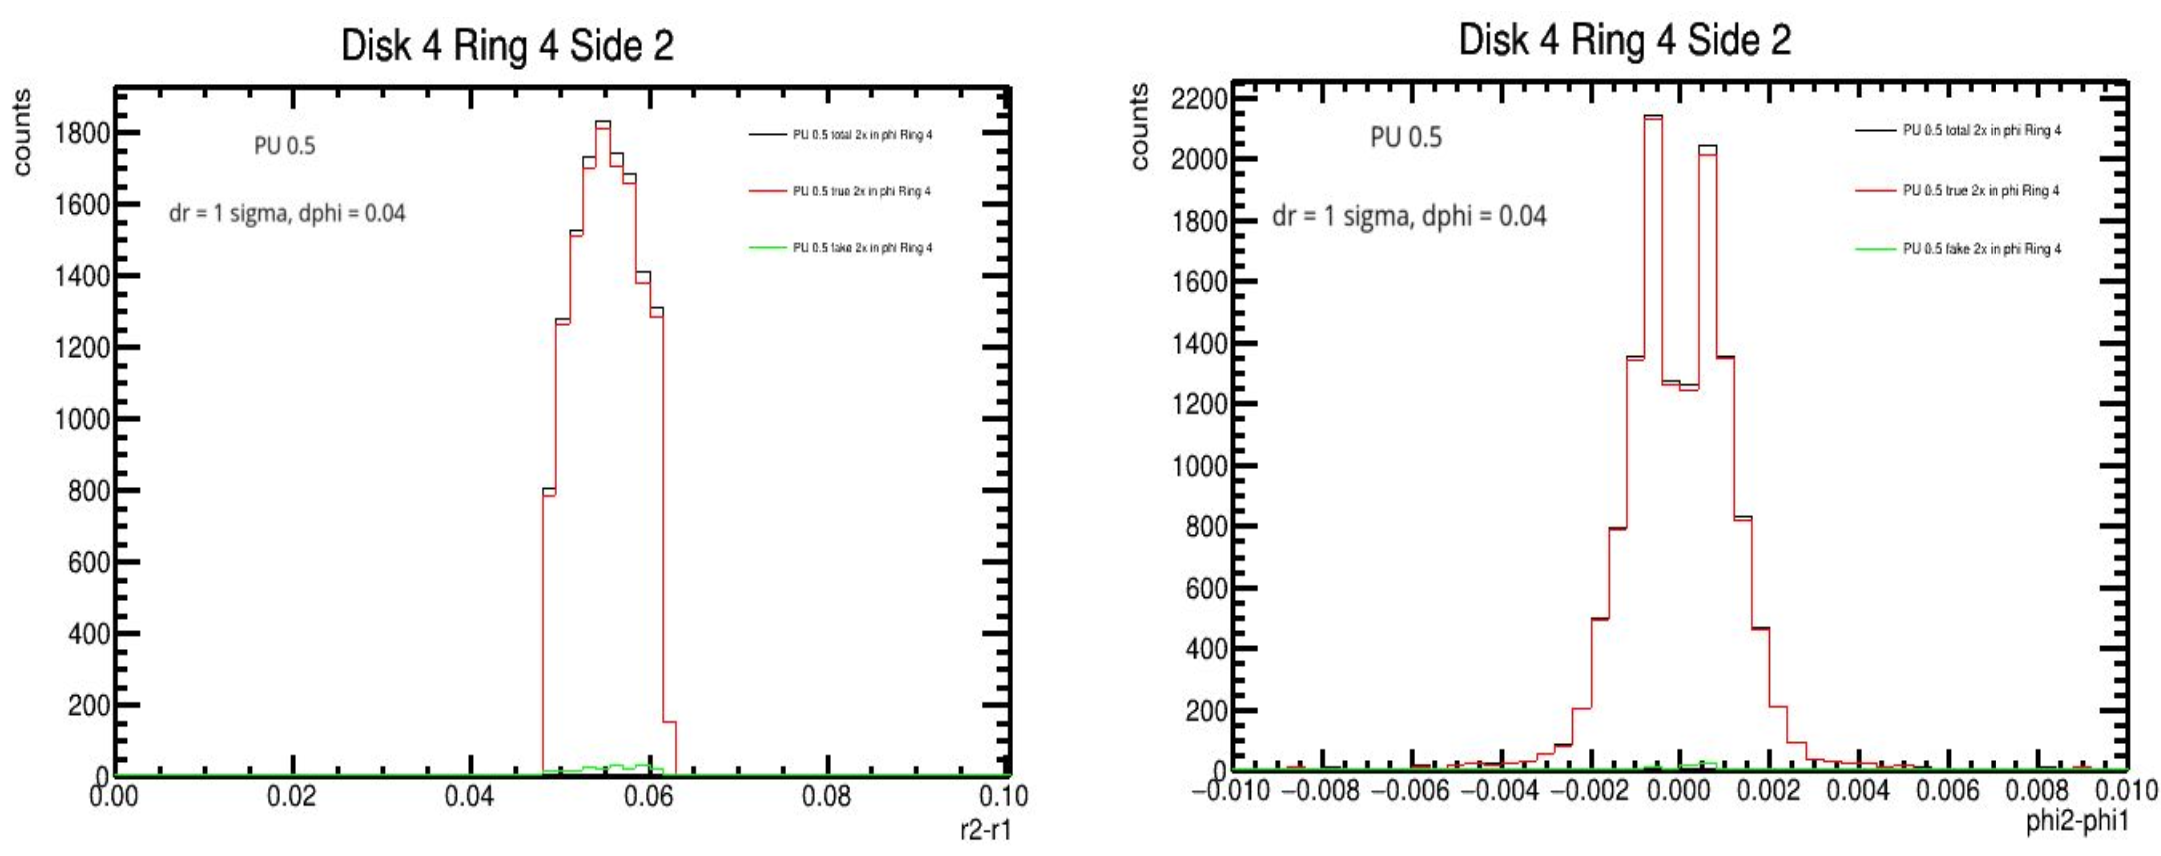
\includegraphics[width=1\textwidth]{ashish_thesis/D4R4S2_dr_dphi_cut.png}
\caption{%
  Distribution of cluster count as a function of dr and dphi variables for pileup 0.5 for disk 4 Ring 4 (+Z). 1 sigma selection on dr and dphi equal to 0.04 are used to minimize fake two fold coincidence clusters.  
}
\label{fig:cluster_ring}
\end{figure}



\begin{figure}[!htp]
\centering
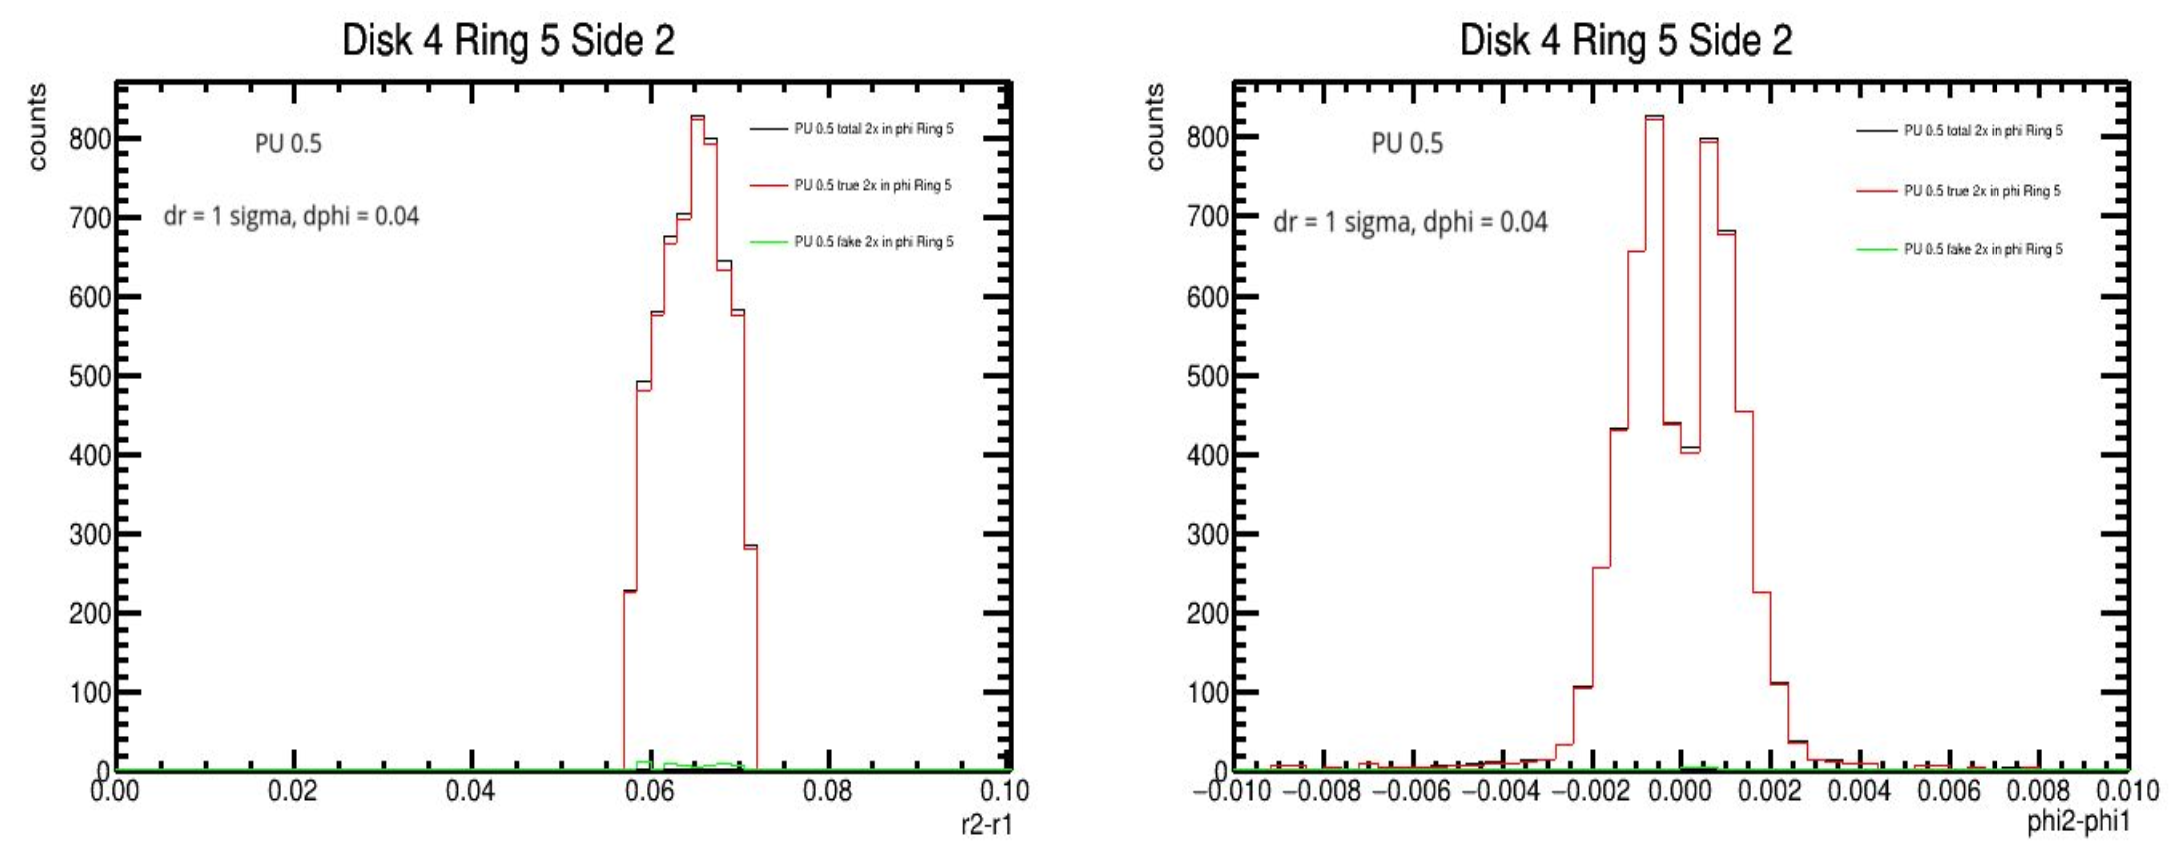
\includegraphics[width=1\textwidth]{ashish_thesis/D4R5S2_dr_dphi_cut.png}
\caption{%
  Distribution of cluster count as a function of dr and dphi variables for pileup 0.5 for disk 4 Ring 5 (+Z). 1 sigma selection on dr and dphi equal to 0.04 are used to minimize fake two fold coincidence clusters.  
}
\label{fig:cluster_ring}
\end{figure}


\begin{figure}[!htp]
\centering
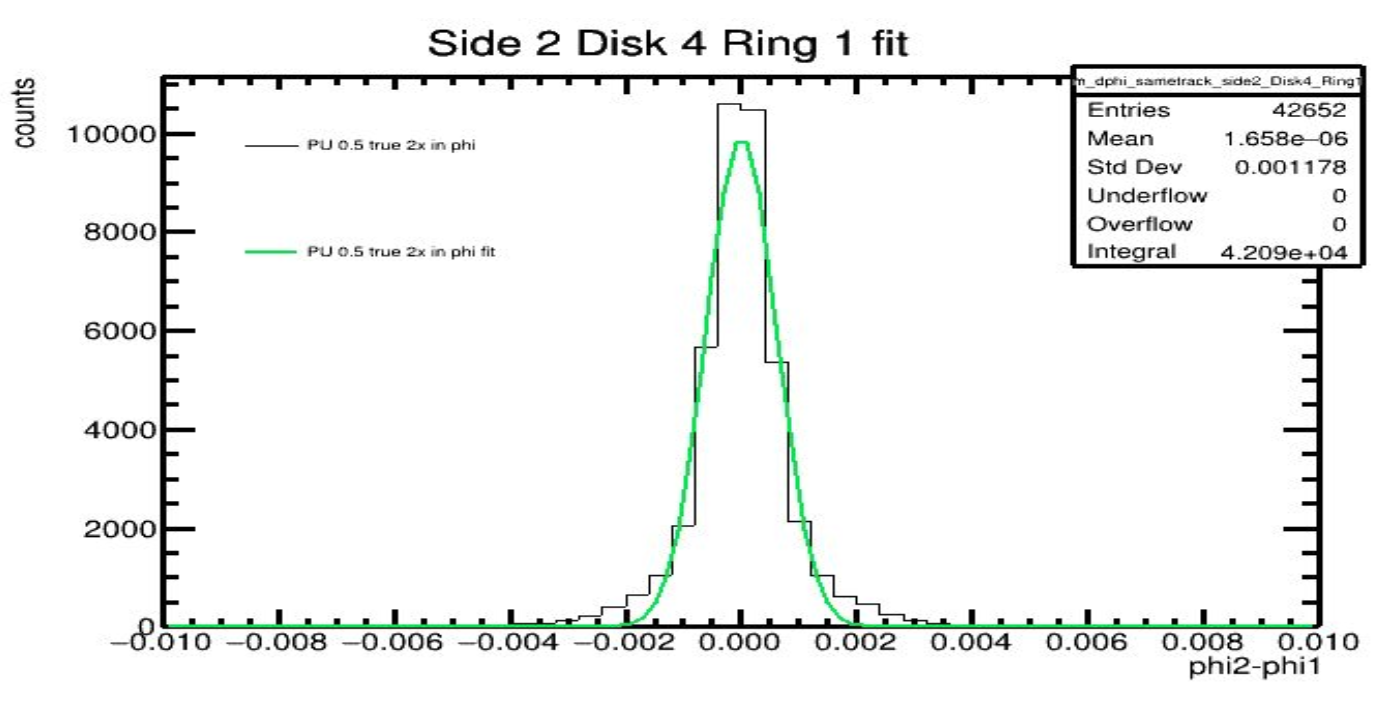
\includegraphics[width=1\textwidth]{ashish_thesis/D4R1S2_fit_PU0p5.png}
\caption{%
  Example fit using single Gaussian function of cluster count as a function of dr variable for pileup 0.5 Disk 4 Ring 1 (+Z).
}
\label{fig:cluster_ring}
\end{figure}


\begin{figure}[!htp]
\centering
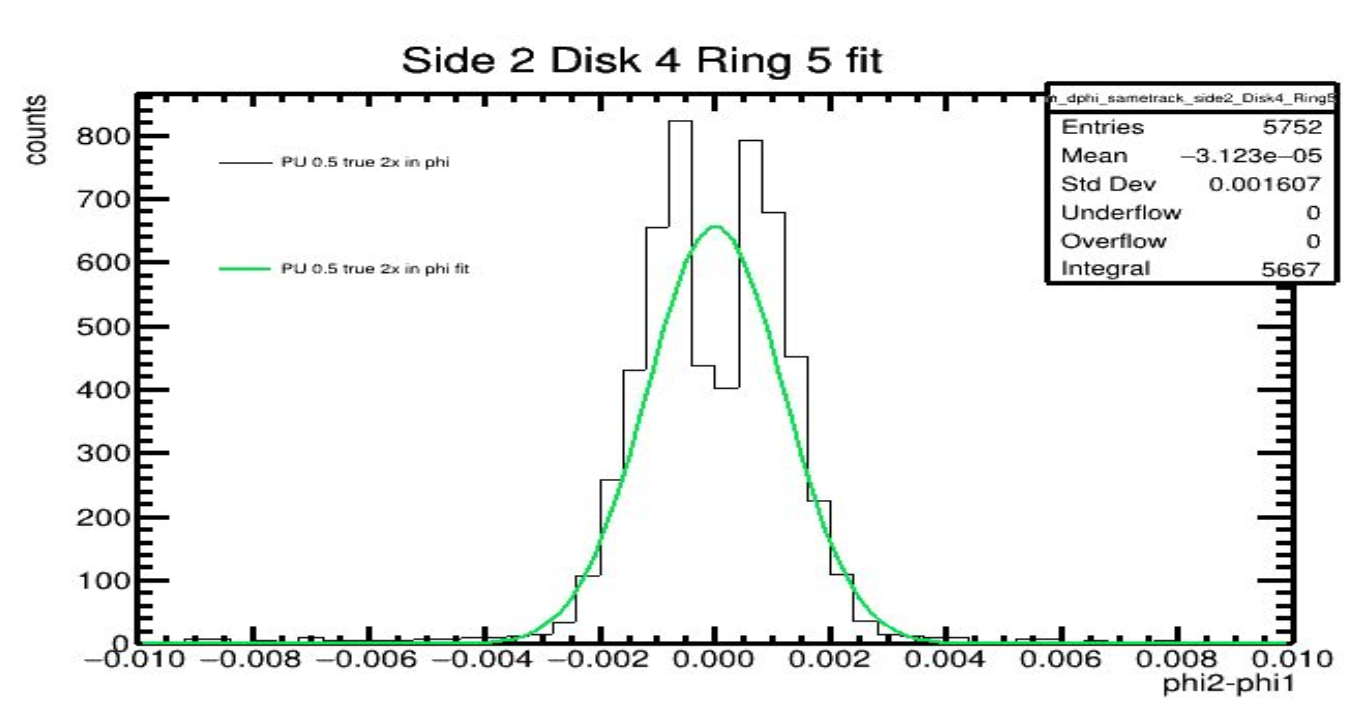
\includegraphics[width=1\textwidth]{ashish_thesis/D4R5_fit_PU0p5.png}
\caption{%
 Example fit using single Gaussian function of cluster count as a function of dr variable for pileup 0.5 Disk 4 Ring 5 (+Z). 
}
\label{fig:cluster_ring}
\end{figure}

\begin{table}[htbp]
  \centering
  \caption{dr cut values for two fold coincidences in phi for all disks and rings}
  \label{tab:disk_values}
  \begin{tabular}{cccccc}
    \textbf{Disk} & \textbf{Ring 1} & \textbf{Ring 2} & \textbf{Ring 3} & \textbf{Ring 4} & \textbf{Ring 5} \\
    \hline
    -1 & 0.00633554 & 0.00709231 & 0.00757662 & 0.008659   & 0.00872148 \\
    -2 & 0.00594206 & 0.00663493 & 0.00718173 & 0.00766371 & 0.00797059 \\
    -3 & 0.00594206 & 0.00663493 & 0.00660603 & 0.00713035 & 0.00679445 \\
    -4 & 0.00530235 & 0.00587692 & 0.00616465 & 0.00661972 & 0.00660599 \\
    1  & 0.00635769 & 0.0071538  & 0.00780034 & 0.00863764 & 0.00883121 \\
    2  & 0.00587583 & 0.00656126 & 0.00700576 & 0.00773345 & 0.00786885 \\
    3  & 0.00557387 & 0.00617934 & 0.00664346 & 0.0070085  & 0.00727192 \\
    4  & 0.0053299  & 0.00586655 & 0.0061499  & 0.00667791 & 0.00678366 \\
  \end{tabular}
\end{table}



\begin{table}[htbp]
  \centering
  \caption{dphi cut values for two fold coincidences in phi for all disks and rings}
  \label{tab:mdphi_cuts_values}
  \begin{tabular}{cccccc}
    \textbf{Disk} & \textbf{Ring 1} & \textbf{Ring 2} & \textbf{Ring 3} & \textbf{Ring 4} & \textbf{Ring 5} \\
    \hline
    -1 & 0.000856727  & 0.00128078   & 0.00151297   & 0.00151297   & 0.0016561    \\
    -2 & 0.000765842  & 0.00110698   & 0.00131104   & 0.00143555   & 0.00150265   \\
    -3 & 0.000684645  & 0.000975385  & 0.00115899   & 0.00126858   & 0.00131598   \\
    -4 & 0.000598839  & 0.000862728  & 0.00104327   & 0.00112621   & 0.00115609   \\
    1  & 0.000877912  & 0.00125898   & 0.0015378    & 0.00164165   & 0.00173015   \\
    2  & 0.00076339   & 0.00110755   & 0.00132174   & 0.00144755   & 0.00150547   \\
    3  & 0.000679543  & 0.000972429  & 0.00116735   & 0.00125955   & 0.00132885   \\
    4  & 0.000609859  & 0.000881345  & 0.00101584   & 0.00112554   & 0.00118477   \\
  \end{tabular}
\end{table}

\begin{table}[htbp]
  \centering
  \caption{dr mean values obtained from fit for two fold coincidences in phi for all disks and rings}
  \label{tab:mdr_cuts_offset_values}
  \begin{tabular}{cccccc}
    \textbf{Disk} & \textbf{Ring 1} & \textbf{Ring 2} & \textbf{Ring 3} & \textbf{Ring 4} & \textbf{Ring 5} \\
    \hline
    -1 & 0.0342041  & 0.0511416 & 0.0676943 & 0.0834355 & 0.0984932 \\
    -2 & 0.0298276  & 0.0445398 & 0.0589828 & 0.0727454 & 0.0853587 \\
    -3 & 0.0260326  & 0.0386608 & 0.05122   & 0.0632478 & 0.0746467 \\
    -4 & 0.0227089  & 0.0336467 & 0.044476  & 0.0551065 & 0.06484   \\
    1  & 0.0341565  & 0.0511018 & 0.0676485 & 0.0835835 & 0.0984028 \\
    2  & 0.0298515  & 0.0444016 & 0.0589681 & 0.0727789 & 0.0854843 \\
    3  & 0.0260239  & 0.0387303 & 0.0511824 & 0.0633755 & 0.0742994 \\
    4  & 0.022729   & 0.0336624 & 0.0445526 & 0.0550466 & 0.0644863 \\
  \end{tabular}
\end{table}


\subsection{TEPX two fold coincidences in R}


\begin{figure}[!htp]
\centering
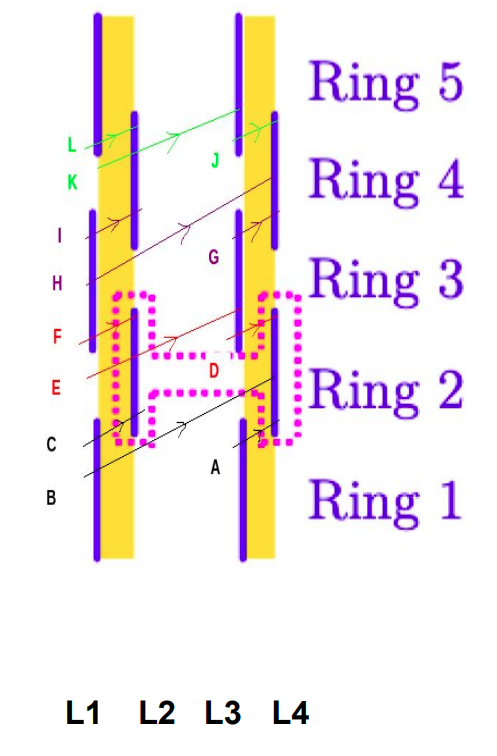
\includegraphics[width=0.5\textwidth]{ashish_thesis/2foldinR.png}
\caption{%
  All possible module overlaps between different rings that can give rise to two fold coincidences in R.
}
\label{fig:cluster_ring}
\end{figure}


\begin{table}[htbp]
\centering
\caption{Various types of two fold coincidences in R in one TEPX double disk with module overlaps and z separation is shown in the table.}
\label{tab:module_connections}
\begin{tabular}{ccc}
\textbf{Two fold in R types} & \textbf{Module overlaps} & \textbf{dz} \\ \hline
A & R1L3-R2L4 & 0.4 \\
B & R1L1-R2L4 & 1.2 \\
C & R1L1-R2L2 & 0.4 \\
D & R3L3-R2L4 & 0.4 \\
E & R2L2-R3L3 & 0.4 \\
F & R3L1-R2L2 & 0.4 \\
G & R3L3-R4L4 & 0.4 \\
H & R3L1-R4L4 & 1.2 \\
I & R3L1-R4L2 & 0.4 \\
J & R5L3-R4L4 & 0.4 \\
K & R4L2-R5L3 & 0.4 \\
L & R5L1-R4L2 & 0.4 \\ 
\end{tabular}
\end{table}


\begin{figure}[!htp]
\centering
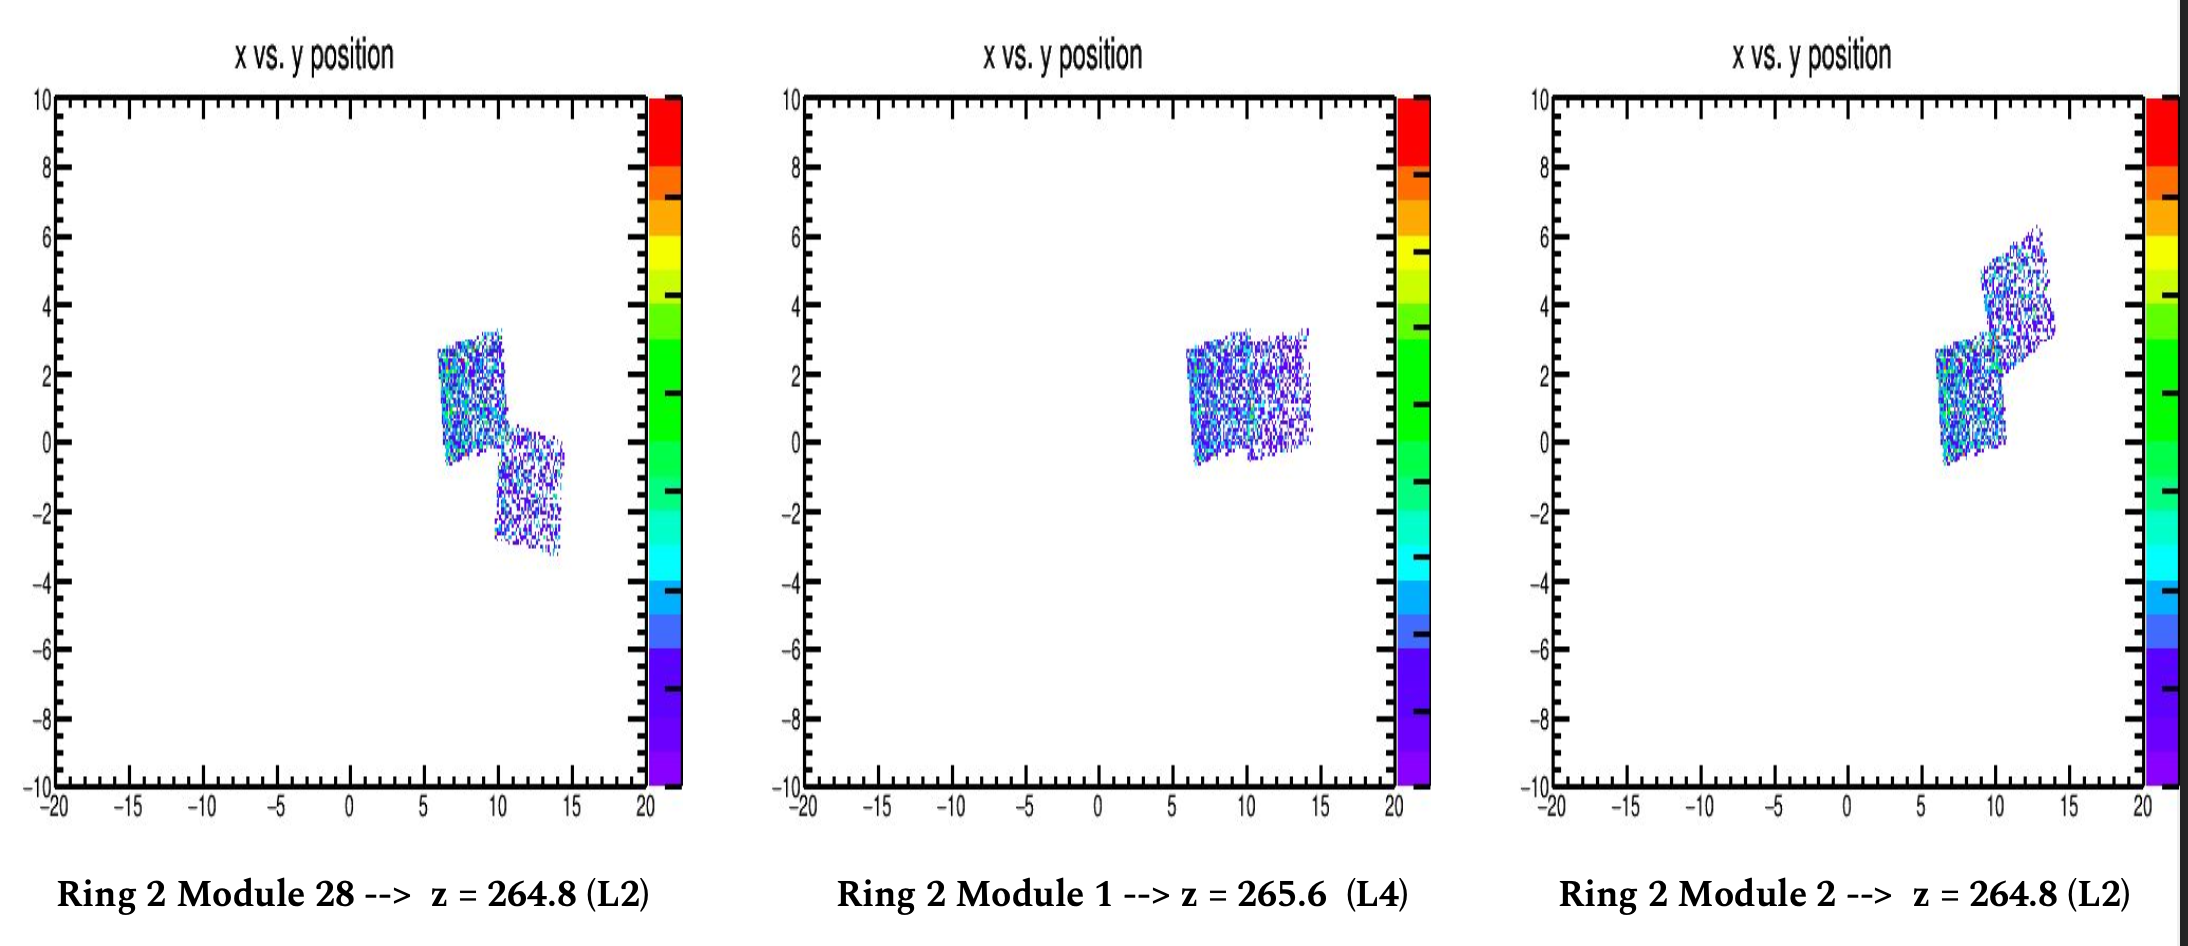
\includegraphics[width=1\textwidth]{ashish_thesis/moduleoverlapinR_1.png}
\caption{%
  Example of module overlap between different ring modules that can give rise to two fold coincidences in R.
}
\label{fig:cluster_ring}
\end{figure}




\begin{figure}[!htp]
\centering
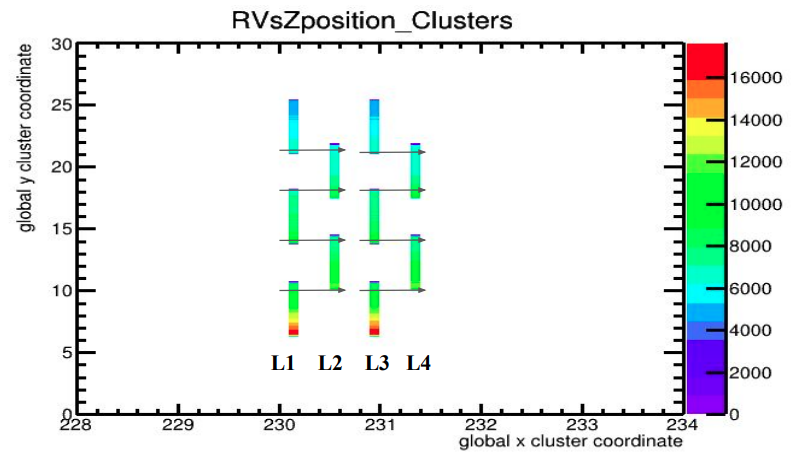
\includegraphics[width=1\textwidth]{ashish_thesis/twofoldinRmethod.png}
\caption{%
  Example of module overlap between different ring modules in the first two and last two layers of one tepx double disk that can give rise to two fold coincidences in R.
}
\label{fig:cluster_ring}
\end{figure}



\begin{figure}[!htp]
\centering
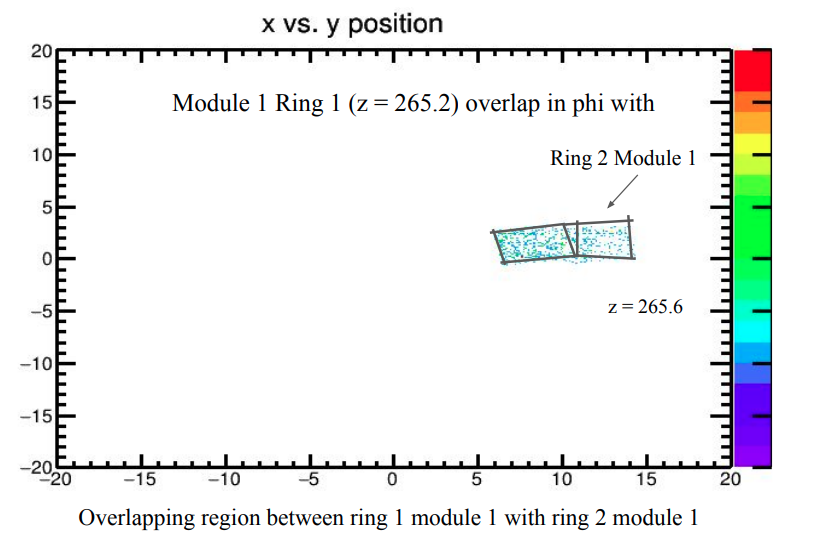
\includegraphics[width=1\textwidth]{ashish_thesis/moduleoverlapfortwofoldinR.png}
\caption{%
   Module overlap between different ring modules that can give rise to two fold coincidences in R.
}
\label{fig:cluster_ring}
\end{figure}



\begin{figure}[!htp]
\centering
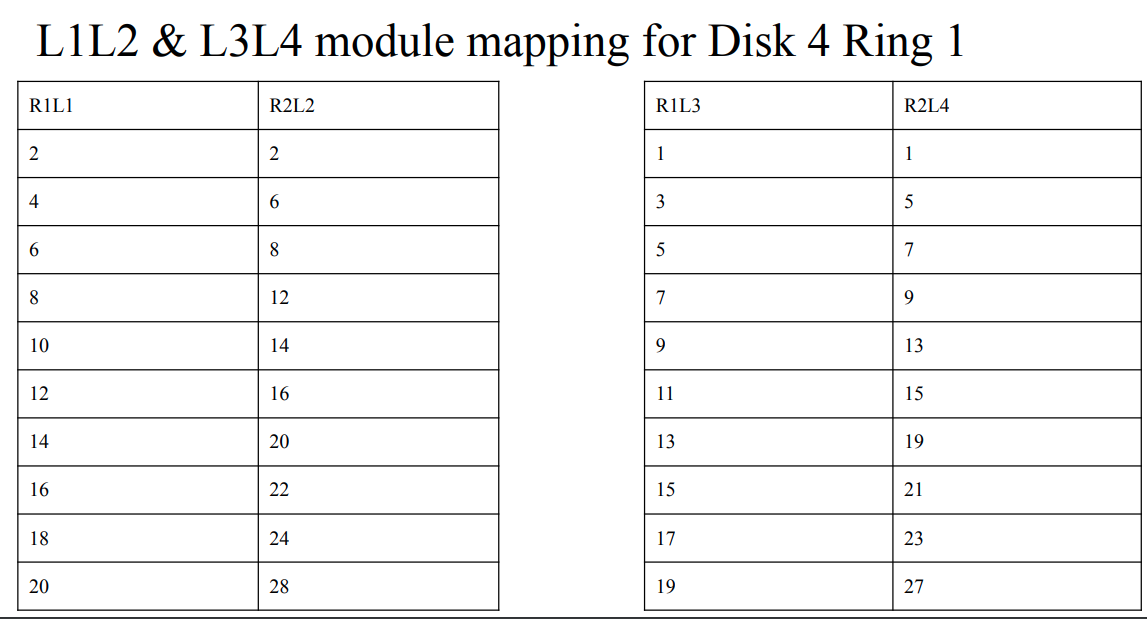
\includegraphics[width=1\textwidth]{ashish_thesis/onetoonemoduleoverlap2xinR_table.png}
\caption{%
   Module overlap between different ring modules that can give rise to two fold coincidences in R.
}
\label{fig:cluster_ring}
\end{figure}



\begin{figure}[!htp]
\centering
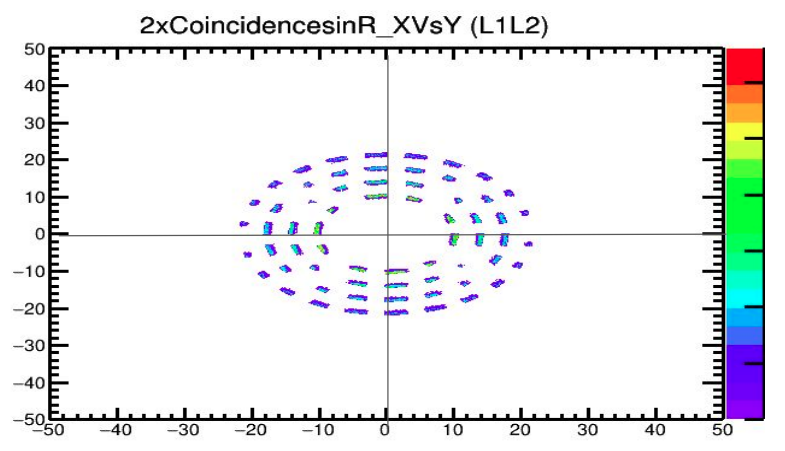
\includegraphics[width=1\textwidth]{ashish_thesis/l1l2_2xinr.png}
\caption{%
   Module overlap between different ring modules that can give rise to two fold coincidences in R.
}
\label{fig:cluster_ring}
\end{figure}

\begin{figure}[!htp]
\centering
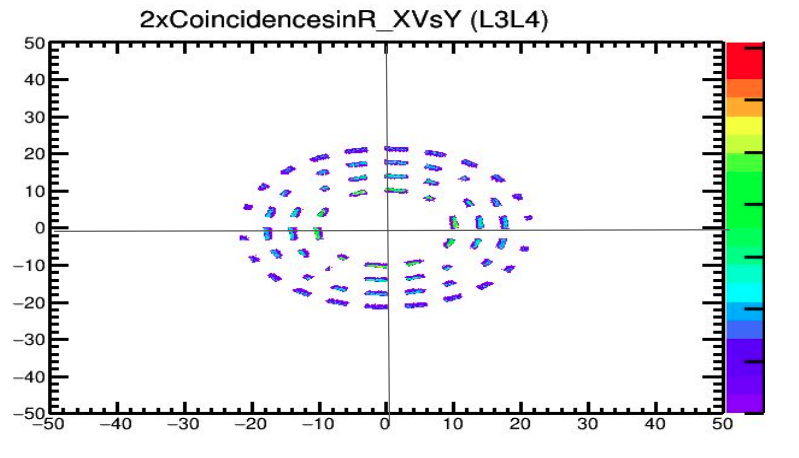
\includegraphics[width=1\textwidth]{ashish_thesis/l3l4_2xinr.png}
\caption{%
   Module overlap between different ring modules that can give rise to two fold coincidences in R.
}
\label{fig:cluster_ring}
\end{figure}



\begin{figure}[!htp]
\centering
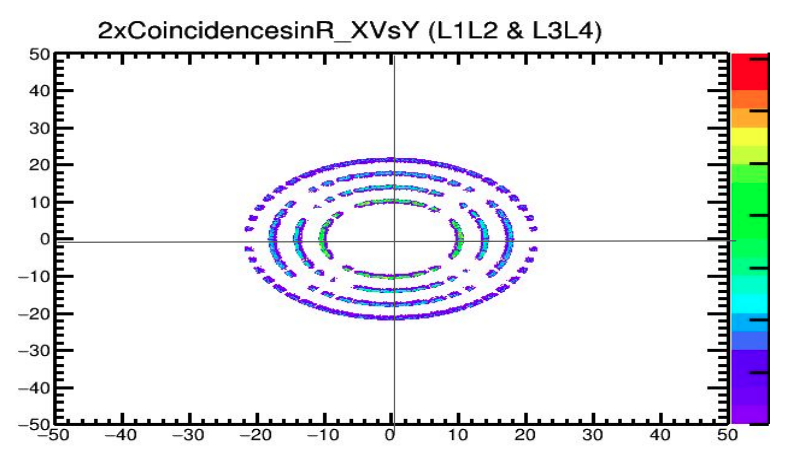
\includegraphics[width=1\textwidth]{ashish_thesis/l1l2_l3l4_2xinr.png}
\caption{%
   Module overlap between different ring modules that can give rise to two fold coincidences in R.
}
\label{fig:cluster_ring}
\end{figure}


\begin{figure}[!htp]
\centering
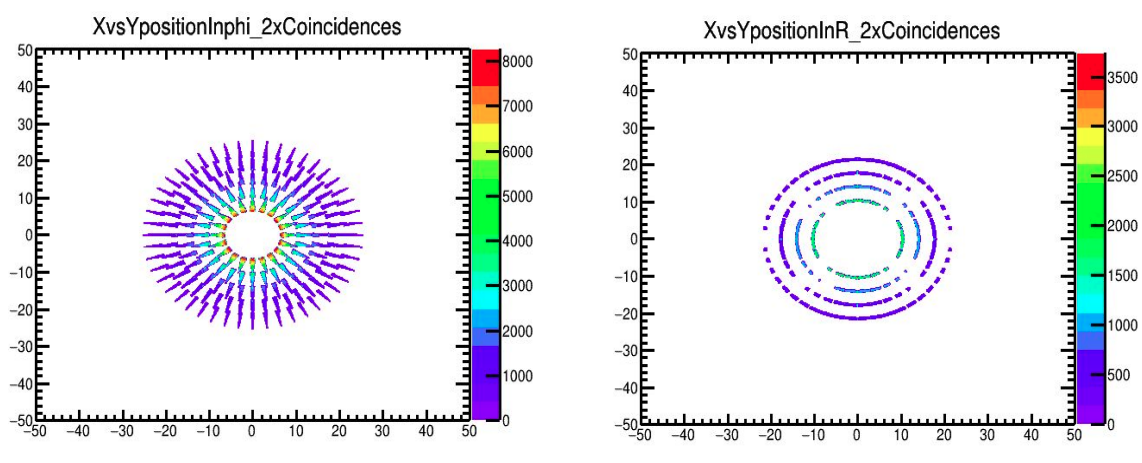
\includegraphics[width=1\textwidth]{ashish_thesis/XY_map_2xinphi_2xinr.png}
\caption{%
   Module overlap between different ring modules that can give rise to two fold coincidences in R.
}
\label{fig:cluster_ring}
\end{figure}



\begin{figure}[!htp]
\centering
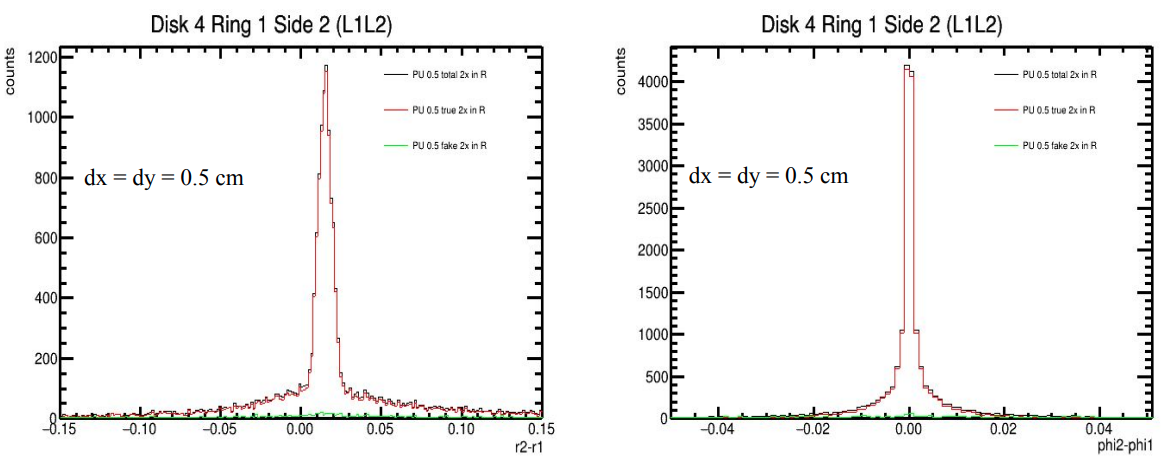
\includegraphics[width=1\textwidth]{ashish_thesis/l1l2_dr_dphi_D4R1S2.png}
\caption{%
   Module overlap between different ring modules that can give rise to two fold coincidences in R.
}
\label{fig:cluster_ring}
\end{figure}

\begin{figure}[!htp]
\centering
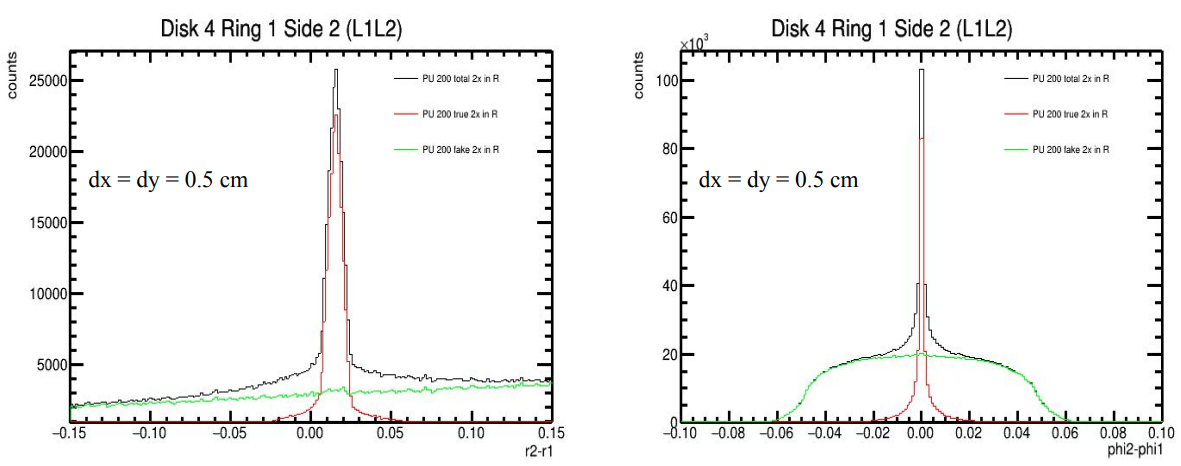
\includegraphics[width=1\textwidth]{ashish_thesis/l1l2_drdphi_2xinr_PU200.png}
\caption{%
   Module overlap between different ring modules that can give rise to two fold coincidences in R.
}
\label{fig:cluster_ring}
\end{figure}


\begin{figure}[!htp]
\centering
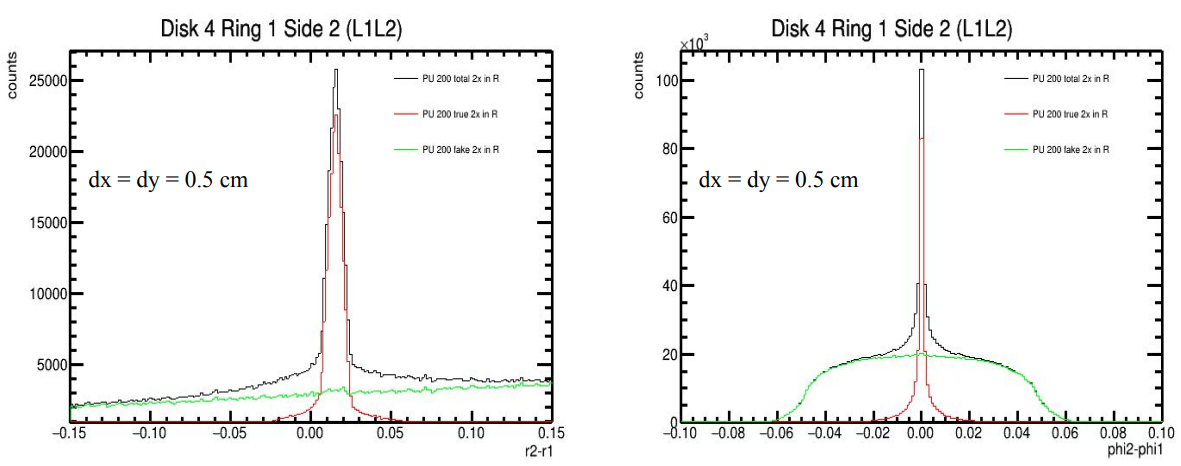
\includegraphics[width=1\textwidth]{ashish_thesis/l1l2_drdphi_2xinr_PU200.png}
\caption{%
   Module overlap between different ring modules that can give rise to two fold coincidences in R.
}
\label{fig:cluster_ring}
\end{figure}



\begin{figure}[!htp]
\centering
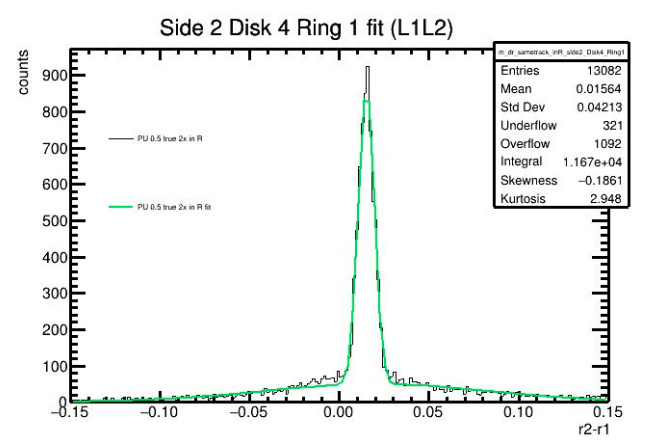
\includegraphics[width=1\textwidth]{ashish_thesis/fit_l1l2_dr_2xinr.png}
\caption{%
   Module overlap between different ring modules that can give rise to two fold coincidences in R.
}
\label{fig:cluster_ring}
\end{figure}



\begin{figure}[!htp]
\centering
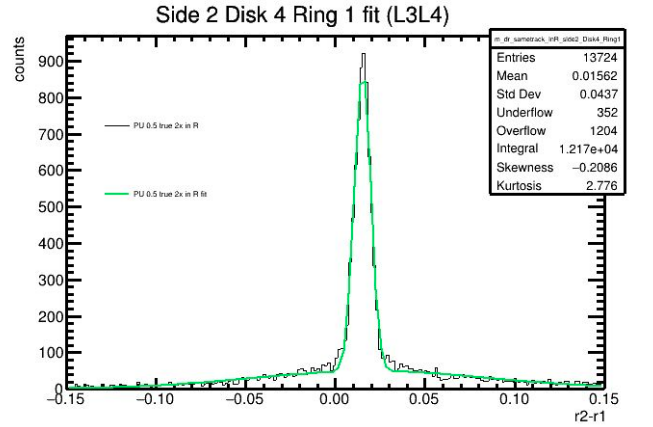
\includegraphics[width=1\textwidth]{ashish_thesis/fit_l3l4_dr_2xinr.png}
\caption{%
   Module overlap between different ring modules that can give rise to two fold coincidences in R.
}
\label{fig:cluster_ring}
\end{figure}



\begin{figure}[!htp]
\centering
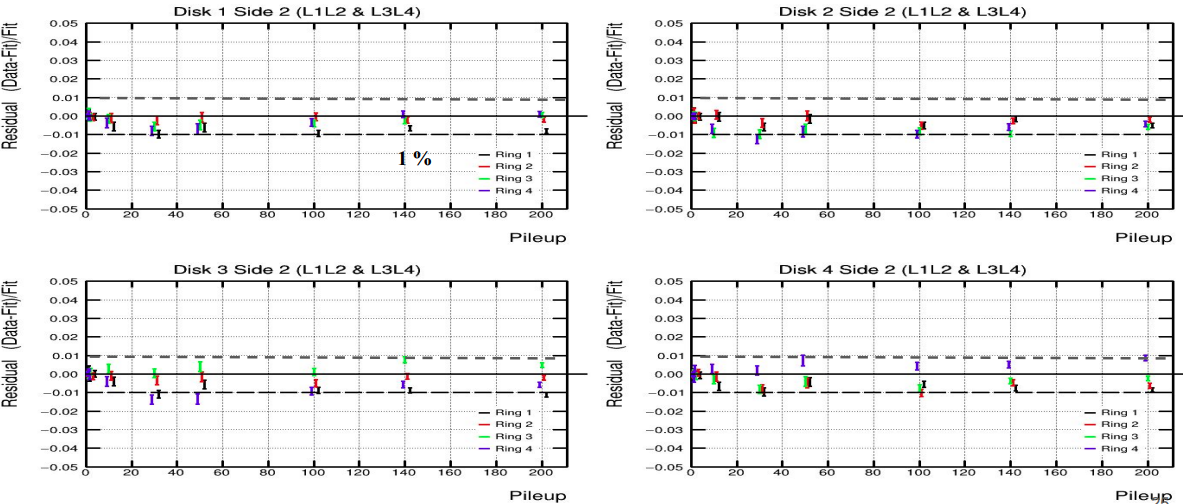
\includegraphics[width=1\textwidth]{ashish_thesis/residuaL_L1L2_L3L4_2xinr.png}
\caption{%
   Module overlap between different ring modules that can give rise to two fold coincidences in R.
}
\label{fig:cluster_ring}
\end{figure}

\begin{comment}

\begin{table}[htbp]
  \centering
  \caption{m\_dr\_cuts\_offset\_InR\_f Values}
  \label{tab:mdr_cuts_offset_InR_f_values}
  \begin{tabular}{cccc}
    \hline
    \textbf{Disk} & \textbf{Ring 1} & \textbf{Ring 2} & \textbf{Ring 3} &  \textbf{Ring 4}\\
    \hline
    -1 & 0.0230881 & 0.0309854 & 0.0387241 & 0.0464962 \\
    -2 & 0.0199761 & 0.0270206 & 0.0338467 & 0.0403068 \\
    -3 & 0.017385  & 0.0233397 & 0.0294101 & 0.0348779 \\
    -4 & 0.0150614 & 0.0202725 & 0.0255259 & 0.0303849 \\
    1  & 0.0229736 & 0.0311421 & 0.0390871 & 0.0468038 \\
    2  & 0.0202136 & 0.0268963 & 0.0337796 & 0.040398  \\
    3  & 0.0174894 & 0.0233893 & 0.0293971 & 0.0351501 \\
    4  & 0.0149661 & 0.020194  & 0.0255051 & 0.0305483 \\
    \hline
  \end{tabular}
\end{table}



\begin{table}[htbp]
  \centering
  \caption{m\_dphi\_cuts\_InR\_f Values}
  \label{tab:mdphi_cuts_InR_f_values}
  \begin{tabular}{cccc}
    \hline
    \textbf{Disk} & \textbf{Ring 1} & \textbf{Ring 2} & \textbf{Ring 3} \\
    \hline
    -1 & 0.000628313 & 0.000828659 & 0.000975585 & 0.00101984  \\
    -2 & 0.000545699 & 0.000722289 & 0.00081899  & 0.000918094 \\
    -3 & 0.000495422 & 0.000649127 & 0.000754224 & 0.000839347 \\
    -4 & 0.000451069 & 0.000604104 & 0.000689508 & 0.000755603 \\
    1  & 0.000627781 & 0.000814669 & 0.000941641 & 0.0010221   \\
    2  & 0.000573352 & 0.000761853 & 0.000851161 & 0.000901014 \\
    3  & 0.000523361 & 0.000662691 & 0.000778358 & 0.000834924 \\
    4  & 0.000471669 & 0.000589938 & 0.000692007 & 0.000750302 \\
    \hline
  \end{tabular}
\end{table}


\begin{table}[htbp]
  \centering
  \caption{m\_dr\_cuts\_InR\_f Values}
  \label{tab:mdr_cuts_InR_f_values}
  \begin{tabular}{cccc}
    \hline
    \textbf{Disk} & \textbf{Ring 1} & \textbf{Ring 2} & \textbf{Ring 3} \\
    \hline
    -1 & 0.00458531 & 0.00466448 & 0.00486059 & 0.0052905  \\
    -2 & 0.00444971 & 0.0046465  & 0.00472138 & 0.00490022 \\
    -3 & 0.00453556 & 0.00471864 & 0.00465781 & 0.00503102 \\
    -4 & 0.00457346 & 0.00458345 & 0.00478342 & 0.00497171 \\
    1  & 0.00448255 & 0.00445856 & 0.00474102 & 0.0051553  \\
    2  & 0.00442349 & 0.00472485 & 0.00474663 & 0.0050426  \\
    3  & 0.00450002 & 0.0045179  & 0.00492058 & 0.00494887 \\
    4  & 0.00444657 & 0.00468584 & 0.00493828 & 0.00488064 \\
    \hline
  \end{tabular}
\end{table}



\begin{table}[htbp]
  \centering
  \caption{m\_dr\_cuts\_InR\_S Values}
  \label{tab:mdr_cuts_InR_S_values}
  \begin{tabular}{cccc}
    \hline
    \textbf{Disk} & \textbf{Ring 1} & \textbf{Ring 2} & \textbf{Ring 3} \\
    \hline
    -1 & 0.00448255 & 0.00445856 & 0.00474102 & 0.0051553  \\
    -2 & 0.00442349 & 0.00472485 & 0.00474663 & 0.0050426  \\
    -3 & 0.00450002 & 0.0045179  & 0.00492058 & 0.00494887 \\
    -4 & 0.00444657 & 0.00468584 & 0.00493828 & 0.00488064 \\
    1  & 0.00458531 & 0.00466448 & 0.00486059 & 0.0052905  \\
    2  & 0.00444971 & 0.0046465  & 0.00472138 & 0.00490022 \\
    3  & 0.00453556 & 0.00471864 & 0.00465781 & 0.00503102 \\
    4  & 0.00457346 & 0.00458345 & 0.00478342 & 0.00497171 \\
    \hline
  \end{tabular}
\end{table}




\begin{table}[htbp]
  \centering
  \caption{m\_dphi\_cuts\_InR\_S Values}
  \label{tab:mdphi_cuts_InR_S_values}
  \begin{tabular}{cccc}
    \hline
    \textbf{Disk} & \textbf{Ring 1} & \textbf{Ring 2} & \textbf{Ring 3} \\
    \hline
    -1 & 0.000627781 & 0.000814669 & 0.000941641 & 0.0010221   \\
    -2 & 0.000573352 & 0.000761853 & 0.000851161 & 0.000901014 \\
    -3 & 0.000523361 & 0.000662691 & 0.000778358 & 0.000834924 \\
    -4 & 0.000471669 & 0.000589938 & 0.000692007 & 0.000750302 \\
    1  & 0.000628313 & 0.000828659 & 0.000975585 & 0.00101984  \\
    2  & 0.000545699 & 0.000722289 & 0.00081899  & 0.000918094 \\
    3  & 0.000495422 & 0.000649127 & 0.000754224 & 0.000839347 \\
    4  & 0.000451069 & 0.000604104 & 0.000689508 & 0.000755603 \\
    \hline
  \end{tabular}
\end{table}

\begin{table}[htbp]
  \centering
  \caption{m\_dr\_cuts\_offset\_InR\_S Values}
  \label{tab:mdr_cuts_offset_InR_S_values}
  \begin{tabular}{cccc}
    \hline
    \textbf{Disk} & \textbf{Ring 1} & \textbf{Ring 2} & \textbf{Ring 3} \\
    \hline
    -1 & 0.0229736 & 0.0311421 & 0.0390871 & 0.0468038 \\
    -2 & 0.0202136 & 0.0268963 & 0.0337796 & 0.040398  \\
    -3 & 0.0174894 & 0.0233893 & 0.0293971 & 0.0351501 \\
    -4 & 0.0149661 & 0.020194  & 0.0255051 & 0.0305483 \\
    1  & 0.0230881 & 0.0309854 & 0.0387241 & 0.0464962 \\
    2  & 0.0199761 & 0.0270206 & 0.0338467 & 0.0403068 \\
    3  & 0.017385  & 0.0233397 & 0.0294101 & 0.0348779 \\
    4  & 0.0150614 & 0.0202725 & 0.0255259 & 0.0303849 \\
    \hline
  \end{tabular}
\end{table}

\end{comment}


%\begin{figure}[!htp]
%\centering
%\includegraphics[width=0.7\textwidth]%{ashish_thesis/events_processed_twofoldcoin_newcuts.png}
%\caption
%\label{fig:cluster_ring}
%\end{figure}


\begin{figure}[!htp]
\centering
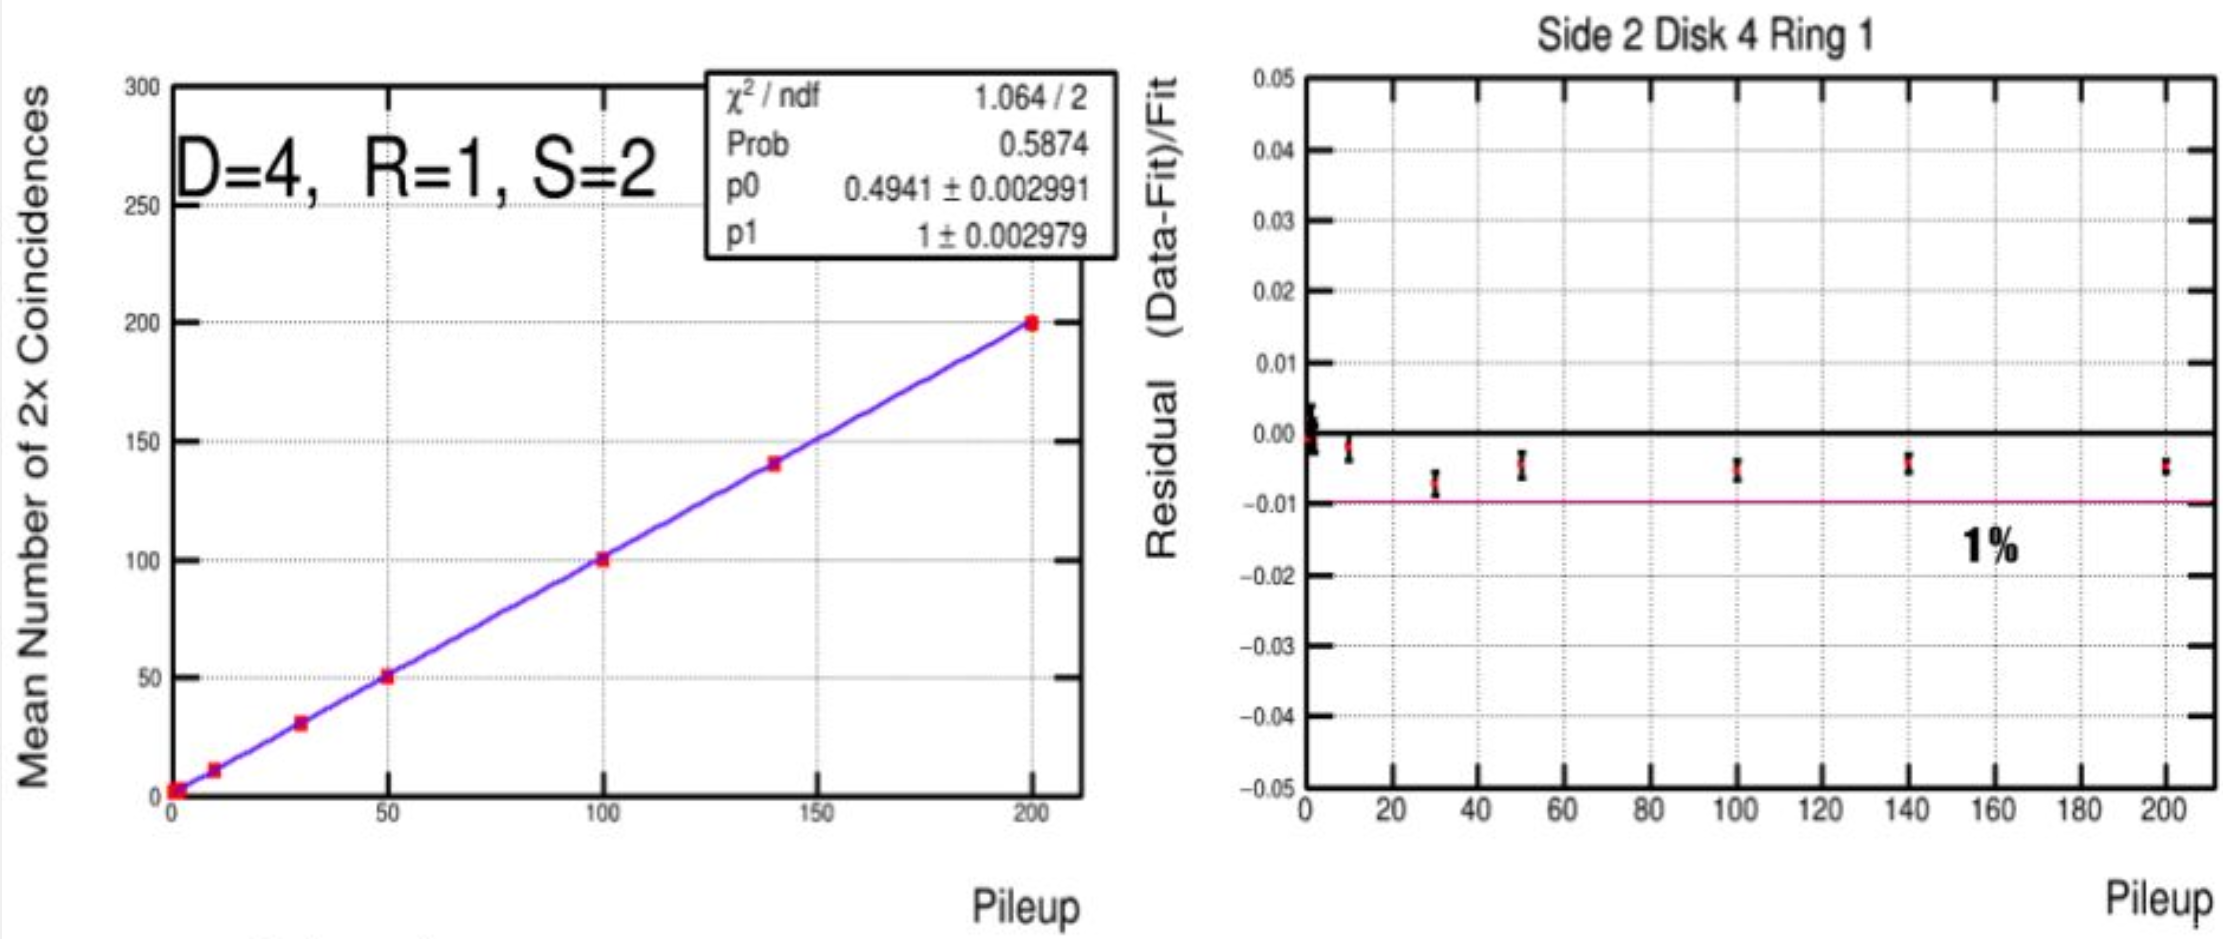
\includegraphics[width=1\textwidth]{ashish_thesis/D4R1S2_linear_fit_twofoldcoin.png}
\caption{%
  Fit two fold coincidences Disk 4 Ring 1 side 2
}
\label{fig:cluster_ring}
\end{figure}


\begin{figure}[!htp]
\centering
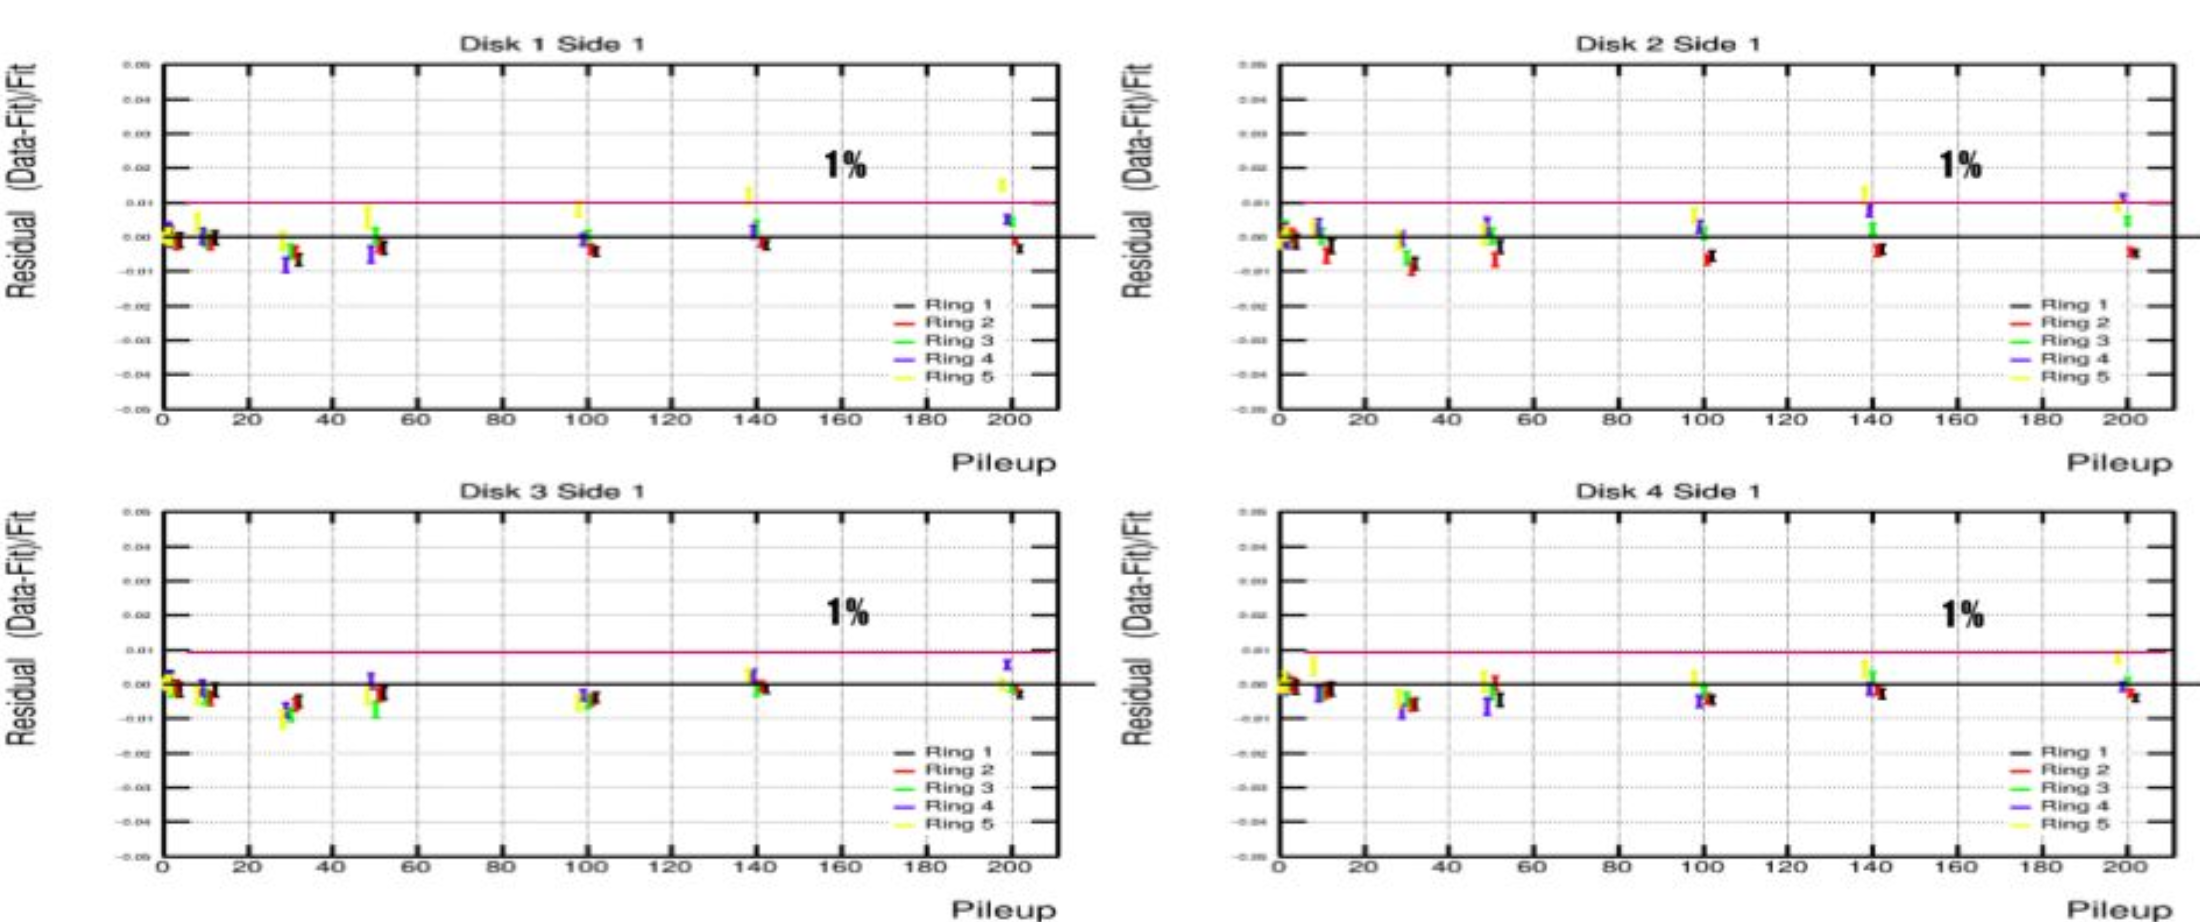
\includegraphics[width=1\textwidth]{ashish_thesis/Alldisk_S1_twofoldcoin_residuals.png}
\caption{%
   fit residual two fold coincidences 
}
\label{fig:cluster_ring}
\end{figure}




\begin{figure}[!htp]
\centering
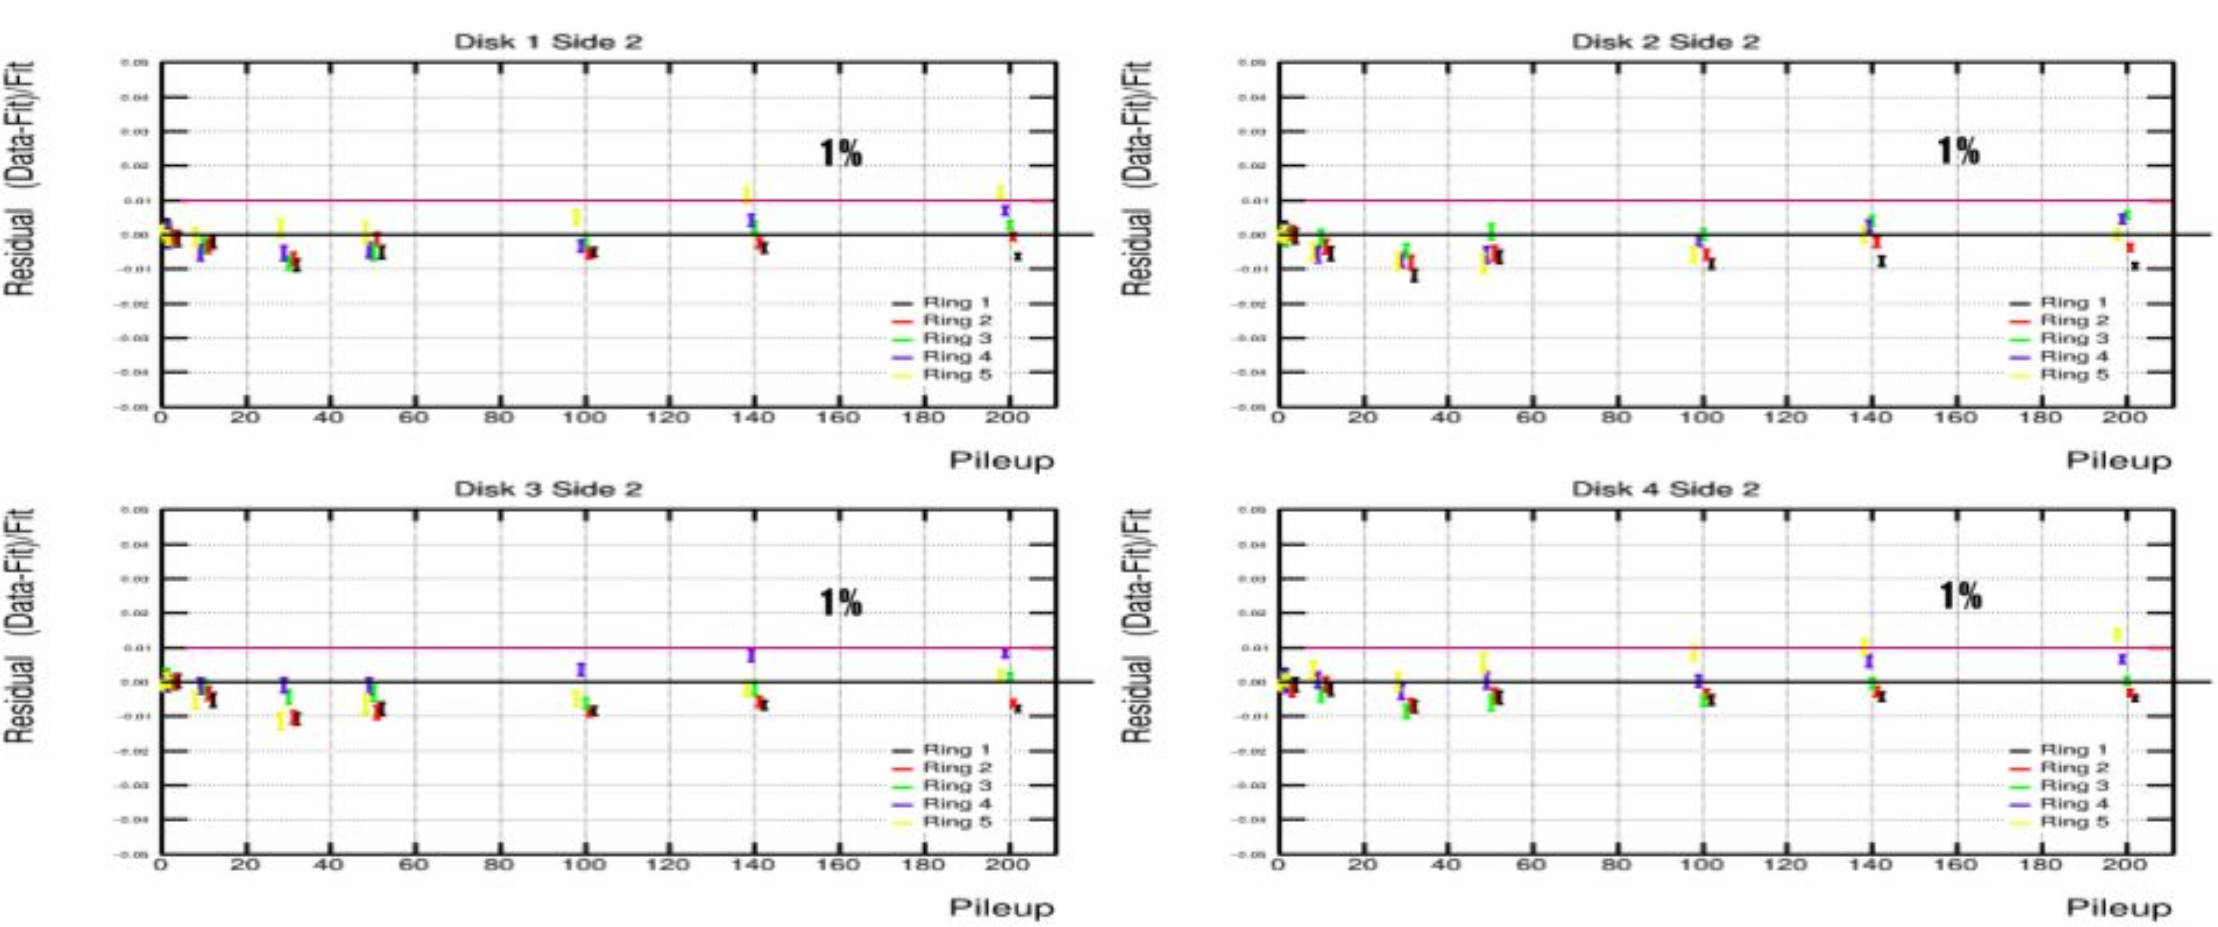
\includegraphics[width=1\textwidth]{ashish_thesis/Alldisk_S2_twofoldcoin_residuals.png}
\caption{%
  fit residual two fold coincidences all disk.
}
\label{fig:cluster_ring}
\end{figure}


\begin{figure}[!htp]
\centering
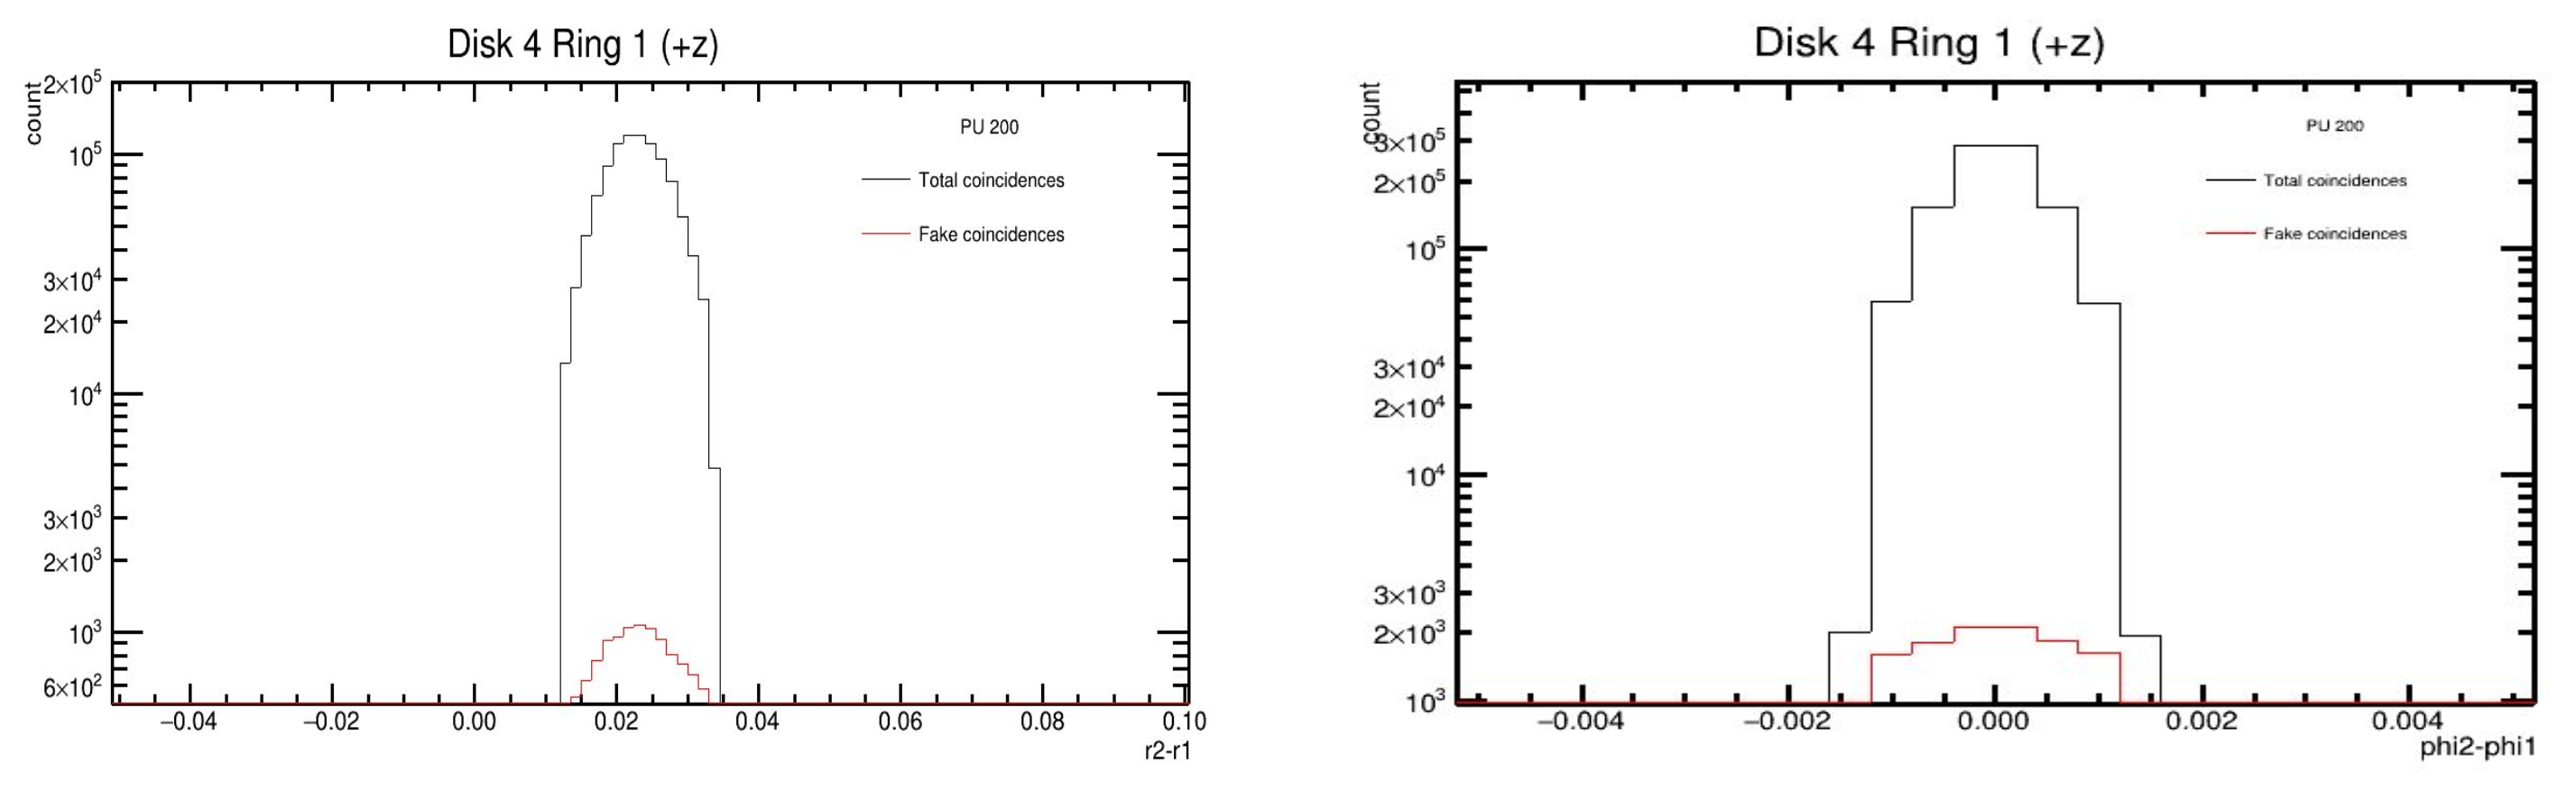
\includegraphics[width=1\textwidth]{ashish_thesis/D4R1_z_dr_dphi_total_fake_twofold.png}
\caption{%
  jhgil
}
\label{fig:cluster_ring}
\end{figure}



\begin{figure}[!htp]
\centering
\includegraphics[width=1\textwidth]{ashish_thesis/D4R5_z_dr_dphi_twofoldcoin_total_fake.png}
\caption{%
   klbjihvb
}
\label{fig:cluster_ring}
\end{figure}



\begin{figure}[!htp]
\centering
\includegraphics[width=0.7\textwidth]{ashish_thesis/fake_rate_D4allring.png}
\caption{%
  lhivbhiv
}
\label{fig:cluster_ring}
\end{figure}


\begin{table}[htbp]
  \centering
  \caption{Sample Table}
  \label{tab:sample}
  \begin{tabular}{cc}
    \textbf{Disk 4} & \textbf{Fake two fold coincidence rate (\%)} \\
    \hline
    Ring 1 &  1.1\\
    Ring 2 &  1.9\\
    Ring 3 &  2.0\\
    Ring 4 &  2.5\\
    Ring 5 &  2.3\\
  \end{tabular}
\end{table}



\begin{table}[htbp]
  \centering
  \caption{Sample Table}
  \label{tab:sample}
  \begin{tabular}{cccc}
    \textbf{Pileup} & \textbf{Fake two fold coincidence in phi rate ()} & \textbf{Fake two fold coincidence in R rate ()} & \textbf{Fake two fold coincidence rate ()} \\
    \hline
   0.5  &  0.78& 0.99 & 0.83 \\
     1& 0.79 &  1.01 &0.85\\
    1.5 &  0.80& 1.02 & 0.86 \\
     2 & 0.79 & 1.02&  0.84\\
    10 &  0.83&  1.04&  0.88\\
     30&  0.94&  1.09&  0.98\\
     50 &  1.04&  1.14&  1.07\\
    100  & 1.31 & 1.29& 1.31\\
     140  & 1.53 & 1.41& 1.50\\
    200   & 1.85 & 1.57 &1.78\\
  \end{tabular}
\end{table}



\begin{table}[htbp]
  \centering
  \caption{Sample Table}
  \label{tab:sample}
  \begin{tabular}{cccc}
    \textbf{Pileup} & \textbf{efficiency for two fold coincidence in phi} & \textbf{Efficiency for Fake two fold coincidence in R} & \textbf{Efficiency for two fold coincidence ()} \\
    \hline 
     0.5  & 99.21 &99.00  &99.16  \\
     1& 99.20 &98.98  & 99.14 \\
    1.5 & 99.19 & 98.97 & 99.13 \\
     2& 99.20 & 98.97 & 99.13 \\
    10 & 99.16 & 98.95 & 99.11 \\
     30& 99.05 & 98.90 & 99.01 \\
     50 & 98.95 & 98.85 & 98.92 \\
    100& 98.68 & 98.70 & 98.68 \\
     140& 98.46 & 98.58 & 98.49 \\
    200 &98.14  & 98.42 &98.21  \\
  \end{tabular}
\end{table}

\begin{figure}[!htp]
\centering
\includegraphics[width=1\textwidth]{ashish_thesis/D4R1_fake_true_ratio.png}
\caption{%
  Ratio of fake and total two fold coincidences for disk 4 ring 1.
}
\label{fig:cluster_ring}
\end{figure}


\begin{figure}[!htp]
\centering
\includegraphics[width=0.7\textwidth]{ashish_thesis/D4R5_fake_true_ratio.png}
\caption{%
  Ratio of fake and total two fold coincidences for disk 4 ring 5.
}
\label{fig:cluster_ring}
\end{figure}

\begin{figure}[H]
  \centering
  \includegraphics[width=0.7\columnwidth]{./2foldinrphi.png}
  \caption{ \onehalfspacing Diagram showing modules overlap between the front (L1 \& L2) and back (L3 \& L4) layers of one double disk of TEPX that creates two fold coincidences in $\phi$ and r.}
  \label{fig:CMS}
\end{figure}

\begin{figure}[H]
  \centering
  \includegraphics[width=0.6\columnwidth]{./23coin.png}
  \caption{\onehalfspacing Example of two and threefold coincidence regions on a portion of a single TEPX disk.}
  \label{fig:CMS}
\end{figure}

\subsection{TEPX linearity}

Linearity is one of the systematic uncertainty in the calculation of instantaneous luminosity and PCC visible cross section $\sigma_{vis}$. A linear relation between the number of clusters and pileup (PU) imply that \\

$<N_{cl/pp}> = \frac{<N_{cl}>}{\mu} = \frac{\sigma_{vis}}{\sigma_{pp}}$ \\

$<N_{cl}> =  \frac{\sigma_{vis}}{\sigma_{pp}} \mu $ \\

Linearity indicates that the PCC visible cross section $\sigma_{vis}$ does not depend on the per bunch instantaneous luminosity (ideal luminometer). In ideal scenario, $\sigma_{vis}$ is not dependent on pileup, but this a potential problem with the luminometer. Linearity results for simulated TEPX clusters and coincidences from low to high pileup values are shown from Fig. 29 to Fig. 40. TEPX luminometer proposed for Phase II shows excellent linearity over entire pileup range. A non-linear relation $<N_{cluster}> = \alpha (PU)^{\gamma}, \gamma \neq 1$ would add non-linear terms in the rate equation $R = \sigma_{vis} L_{inst}$  and cause $\sigma_{vis}$ to vary with the per bunch instantaneous luminosity and pileup values.


\begin{figure}[H]
  \centering
  \includegraphics[width=1\columnwidth]{./totalclusters.png}
  \caption{\onehalfspacing Left: Simulated mean number of clusters for all entire TEPX detector as a function of pileup. A line is fitted between pileup values of 0 and 2, and then extrapolated up to a pileup of 200. Right: Deviation from linearity for clusters for entire TEPX detector. The non-linearity is calculated as the relative difference between the data points and the values of the fit function at the respective pileup value. Non-linearity is within 1 \% for entire pileup range. Pileup 200 corresponds to High Luminosity (HL)-LHC environment.}
  \label{fig:CMS}
\end{figure}



\begin{figure}[H]
  \centering
  \includegraphics[width=1\columnwidth]{./clustersD4R1.png}
  \caption{\onehalfspacing Left: Simulated mean number of clusters for TEPX Disk 4 Ring 1 as a function of pileup. Right: Deviation from linearity for clusters for TEPX Disk 4 Ring 1. The non-linearity is calculated as the relative difference between the data points and the values of the fit function at the respective pileup value.}
  \label{fig:CMS}
\end{figure}



\begin{figure}[H]
  \centering
  \includegraphics[width=1 \columnwidth]{./clustersperdisk+z.png}
  \caption{Left: Simulated mean number of clusters for +z side TEPX disks as a function of pileup. Right: Deviation from linearity for clusters for +z side TEPX disks.}
  \label{fig:CMS}
\end{figure}




\begin{figure}[H]
  \centering
  \includegraphics[width=1\columnwidth]{./clustersperringD+4.png}
  \caption{Left: Simulated mean number of clusters for +z side TEPX Disk 4 all rings as a function of pileup. Ring 1 has highest slope and Ring 5 has least slope. Right: Deviation from linearity for clusters for TEPX Disk +4 all rings. Non-linearity is within $1\%$ for all rings over entire pileup range.}
  \label{fig:CMS}
\end{figure}


\begin{figure}[H]
  \centering
  \includegraphics[width=1 \columnwidth]{./totalcoincidences.png}
  \caption{Left: Simulated mean number of coincidences in $\phi$ and r for all entire TEPX detector as a function of pileup. A line is fitted between pileup values of 0 and 2, and then extrapolated up to a pileup of 200. Right: Deviation from linearity for coincidence in $\phi$ and r for entire TEPX detector. The non-linearity is calculated as the relative difference between the data points and the values of the fit function at the respective pileup value. Non-linearity is within 1 \% for entire pileup range. Pileup 200 corresponds to High Luminosity (HL)-LHC environment.}
  \label{fig:CMS}
\end{figure}


\begin{figure}[H]
  \centering
  \includegraphics[width=1\columnwidth]{./totalcoincidencesD4R1.png}
  \caption{Left: Simulated mean number of coincidences in $\phi$ and r for TEPX Disk 4 Ring 1 as a function of pileup. Right: Deviation from linearity for coincidences in $\phi$ and r for TEPX Disk 4 Ring 1. The non-linearity is calculated as the relative difference between the data points and the values of the fit function at the respective pileup value.}
  \label{fig:CMS}
\end{figure}





\begin{figure}[H]
  \centering
  \includegraphics[width=1\columnwidth]{./coincidencesperdisk+z.png}
  \caption{Left: Simulated mean number of coincidences in $\phi$ and r for +z side TEPX disks as a function of pileup. Right: Deviation from linearity for coincidences in $\phi$ and r for +z side TEPX disks.}
  \label{fig:CMS}
\end{figure}


\begin{figure}[H]
  \centering
  \includegraphics[width=1\columnwidth]{./coincidencesinphiD4R1z+.png}
  \caption{Left: Simulated mean number of coincidences in $\phi$ for TEPX +z side Disk 4 Ring 1 as a function of pileup. Right: Deviation from linearity for coincidences in $\phi$ for TEPX +z side Disk 4 Ring 1. The non-linearity is calculated as the relative difference between the data points and the values of the fit function at the respective pileup value.}
  \label{fig:CMS}
\end{figure}



\begin{figure}[H]
  \centering
  \includegraphics[width=1\columnwidth]{./coincidencesinrD4R1z+.png}
  \caption{Left: Simulated mean number of coincidences in r for TEPX +z side Disk 4 Ring 1 as a function of pileup. Right: Deviation from linearity for coincidences in r for TEPX +z side Disk 4 Ring 1. The non-linearity is calculated as the relative difference between the data points and the values of the fit function at the respective pileup value.}
  \label{fig:CMS}
\end{figure}





\begin{figure}[H]
  \centering
  \includegraphics[width=1\columnwidth]{./coincidencesperringD+4.png}
  \caption{Left: Simulated mean number of coincidences in $\phi$ and r for +z side TEPX Disk 4 per ring as a function of pileup. Ring 1 has highest slope and Ring 5 has least slope. Right: Deviation from linearity for coincidences in $\phi$ and r for +z side TEPX Disk 4 per ring. Non-linearity is within 1\% for all rings over entire pileup range.}
  \label{fig:CMS}
\end{figure}








\begin{figure}[H]
  \centering
  \includegraphics[width=1\columnwidth]{./coincidencesinphiperringD+4.png}
  \caption{Left: Simulated mean number of coincidences in $\phi$ for +z side TEPX Disk 4 per ring as a function of pileup. Ring 1 has highest slope and Ring 5 has least slope. Right: Deviation from linearity for coincidences in $\phi$ for +z side TEPX Disk 4 per ring. Non-linearity is within 1\% for all rings over entire pileup range.}
  \label{fig:CMS}
\end{figure}





\begin{figure}[H]
  \centering
  \includegraphics[width=1\columnwidth]{./coincidencesinrperringD+4.png}
  \caption{Left: Simulated mean number of coincidences in r for +z side TEPX Disk 4 per ring as a function of pileup. Ring 1 has highest slope and Ring 5 has least slope. Right: Deviation from linearity for coincidences in r for +z side TEPX Disk 4 per ring. Non-linearity is within $1\%$ for all rings over entire pileup range.}
  \label{fig:CMS}
\end{figure}


\subsection{Statistical precision for TEPX luminometer}
Statistical precision is another uncertainty that need to be considered for precise luminosity measurement. It must be kept minimal to achieve 1 $\%$ accuracy for HL-LHC luminosity measurement.

Relative statistical uncertainty in $\%$ = $\frac{\sqrt{N}}{N} \times 100$ \\

where N = (Number of counts per event)$\times$(Trigger Frequency)$\times$(Time Integration period). 

\newpage
\begin{flushleft} 
Table 1: Expected statistical precision (in $\%$) in head-on collisions during typical vdM conditions with pileup of 0.5 for TEPX clusters and two fold coincidences over different integration time period.
\end{flushleft} 
\begin{center}
\scalebox{1}{
\begin{tabular}{|l | c | c | c |c|}
\hline
 vdM (PU 0.5) & Readout Rate (kHz) &1 bx, 1s & 1 bx, 30s & 100 bx, 30s\\
\hline
TEPXD4R1 Clusters&1000&1.82&0.332 & 0.0332\\
\hline
TEPXD4R1 2x Coincidences in phi &1000&5.98&1.09 & 0.109\\
\hline
TEPXD4R1 2x Coincidences in r &1000&11.1&2.02 & 0.202\\
\hline
TEPXD4R1 2x Coincidences &1000&5.27&0.962 & 0.0962\\
\hline
TEPX Clusters&500&0.709&0.129 & 0.0129\\
\hline
TEPX 2x Coincidences in phi &500&2.65&0.485 & 0.0485\\
\hline
TEPX 2x Coincidences in r &500&4.59&0.838 & 0.0838\\
\hline
TEPX 2x Coincidences &500&2.3&0.42 & 0.042\\
\hline
\end{tabular}}
\end{center}

\begin{flushleft} 
  Table 2: Expected statistical precision (in $\%$) in head-on collisions during physics conditions with pileup of 200 for TEPX clusters and two fold coincidences over different integration time period.
  \end{flushleft} 
\begin{center}
\scalebox{1}{
\begin{tabular}{|l | c | c | c |c |}
\hline
Algorithm & Readout Rate (kHz)& 1 bx, 1s &2500 bx, 1s   & 2500 bx, 1 LS \\
\hline
TEPXD4R1 Clusters&825&0.1&0.002&0.000414\\
\hline
TEPXD4R1 2x Coincidences in phi &825&0.329&0.00659&0.00136\\
\hline
TEPXD4R1 2x Coincidences in r &825&0.61&0.0122&0.00252\\
\hline
TEPXD4R1 2x Coincidences  &825&0.29&0.0058&0.0012\\
\hline
TEPX Clusters &75&0.0915&0.00183&0.000379\\
\hline
TEPX 2x Coincidences in phi &75&0.343&0.00685&0.00142\\
\hline
TEPX 2x Coincidences in r &75&0.593&0.0119&0.00245\\
\hline
TEPX 2x Coincidences &75&0.297&0.00594&0.00123\\
\hline
\end{tabular}}
\end{center}


\section{Summary of the planned upgrade schedule}

The Phase II upgrade of the CMS detector is a major project that will take several years to complete. The design and development of the upgraded components is currently underway, and the installation of the new detectors and electronics is scheduled to take place over the next few years. The commissioning and testing phase will be critical to ensure that the upgraded detector is functioning properly, and full operation of the upgraded CMS detector is expected to begin in 2026. Planned upgrade schedule for the Phase II upgrade of the CMS detector:

\begin{itemize}

\item 2018-2024: Design and development of the upgraded components, including the new pixel and strip detectors, timing layer, and data acquisition system.

\item 2022-2023: Installation of the new carbon-fiber support structure for the upgraded tracker.

\item 2023-2025: Installation of the new detectors and electronics in the CMS detector, including the pixel and strip detectors, timing layer, and data acquisition system.

\item 2025-2026: Commissioning and testing of the upgraded detector.

\item 2026: Full operation of the upgraded CMS detector.

\end{itemize}






\begin{comment}

\begin{figure}[!htp]
\centering
\includegraphics[width=0.7\textwidth]{ashish_thesis/xvsy_cluster.png}
\caption{%
  cluster map tepx 
}
\label{fig:cluster_xvsy}
\end{figure}


\begin{figure}[!htp]
\centering
\includegraphics[width=0.7\textwidth]{ashish_thesis/cluster_ring.png}
\caption{%
  cluster per event ring tepx 
}
\label{fig:cluster_ring}
\end{figure}


\begin{figure}[!htp]
\centering
\includegraphics[width=0.7\textwidth]{ashish_thesis/tepx_dataset.png}
\caption{%
  cluster per event ring tepx 
}
\label{fig:cluster_ring}
\end{figure}


\begin{figure}[!htp]
\centering
\includegraphics[width=0.7\textwidth]{ashish_thesis/tepx_events_processed.png}
\caption{%
  cluster per event ring tepx 
}
\label{fig:cluster_ring}
\end{figure}


\begin{figure}[!htp]
\centering
\includegraphics[width=0.7\textwidth]{ashish_thesis/tepx_cluster_pu100.png}
\caption{%
  cluster per event ring tepx 
}
\label{fig:cluster_ring}
\end{figure}

\begin{figure}[!htp]
\centering
\includegraphics[width=0.7\textwidth]{ashish_thesis/clusters_tepx_disk4.png}
\caption{%
  cluster per event ring tepx 
}
\label{fig:cluster_ring}
\end{figure}


\begin{figure}[!htp]
\centering
\includegraphics[width=0.7\textwidth]{ashish_thesis/clusters_tepx_pu10_allrings.png}
\caption{%
  cluster per event ring tepx 
}
\label{fig:cluster_ring}
\end{figure}

\begin{figure}[!htp]
\centering
\includegraphics[width=0.7\textwidth]{ashish_thesis/lowpu_clusters_fit_D4R1.png}
\caption{%
  cluster per event ring tepx 
}
\label{fig:cluster_ring}
\end{figure}



\begin{figure}[!htp]
\centering
\includegraphics[width=0.7\textwidth]{ashish_thesis/fit_extrapol_D4R1.png}
\caption{%
  cluster per event ring tepx 
}
\label{fig:cluster_ring}
\end{figure}

\begin{figure}[!htp]
\centering
\includegraphics[width=0.7\textwidth]{ashish_thesis/twofoldcoin_D4_allring (1).png}
\caption{%
  cluster per event ring tepx 
}
\label{fig:cluster_ring}
\end{figure}


\begin{figure}[!htp]
\centering
\includegraphics[width=0.7\textwidth]{ashish_thesis/twofold_geometry_pu30.png}
\caption{%
  cluster per event ring tepx 
}
\label{fig:cluster_ring}
\end{figure}



\begin{figure}[!htp]
\centering
\includegraphics[width=0.7\textwidth]{ashish_thesis/lowpufit_twofold_D4R1.png}
\caption{%
  cluster per event ring tepx 
}
\label{fig:cluster_ring}
\end{figure}



\begin{figure}[!htp]
\centering
\includegraphics[width=0.7\textwidth]{ashish_thesis/twofoldcoincidences_extrapolation_D4R1.png}
\caption{%
  cluster per event ring tepx 
}
\label{fig:cluster_ring}
\end{figure}


\begin{figure}[!htp]
\centering
\includegraphics[width=0.7\textwidth]{ashish_thesis/twofold_residual_D4R1.png}
\caption{%
  cluster per event ring tepx 
}
\label{fig:cluster_ring}
\end{figure}


\begin{figure}[!htp]
\centering
\includegraphics[width=0.7\textwidth]{ashish_thesis/events_per_file_tepx_sim.png}
\caption{%
  cluster per event ring tepx 
}
\label{fig:cluster_ring}
\end{figure}


\begin{figure}[!htp]
\centering
\includegraphics[width=0.7\textwidth]{ashish_thesis/clusters_D4R1_low_allPU.png}
\caption{%
  cluster per event ring tepx 
}
\label{fig:cluster_ring}
\end{figure}



\begin{figure}[!htp]
\centering
\includegraphics[width=0.7\textwidth]{ashish_thesis/twofoldcoin_low_allpu_D4R1.png}
\caption{%
  cluster per event ring tepx 
}
\label{fig:cluster_ring}
\end{figure}



\begin{figure}[!htp]
\centering
\includegraphics[width=0.7\textwidth]{ashish_thesis/threefoldcoin_D4_PU100.png}
\caption{%
  cluster per event ring tepx 
}
\label{fig:cluster_ring}
\end{figure}


\begin{figure}[!htp]
\centering
\includegraphics[width=0.7\textwidth]{ashish_thesis/threefoldcoin_D4_allpu.png}
\caption{%
  cluster per event ring tepx 
}
\label{fig:cluster_ring}
\end{figure}

\begin{figure}[!htp]
\centering
\includegraphics[width=0.7\textwidth]{ashish_thesis/threefoldcoin_D4_lowPU.png}
\caption{%
  cluster per event ring tepx 
}
\label{fig:cluster_ring}
\end{figure}













\begin{figure}[!htp]
\centering
\includegraphics[width=0.7\textwidth]{ashish_thesis/stat_prec_d4r1.png}
\caption{%
  cluster per event ring tepx 
}
\label{fig:cluster_ring}
\end{figure}














\begin{figure}[!htp]
\centering
\includegraphics[width=0.7\textwidth]{ashish_thesis/cut_optimization_twofold.png}
\caption{%
  cluster per event ring tepx 
}
\label{fig:cluster_ring}
\end{figure}



\begin{figure}[!htp]
\centering
\includegraphics[width=0.7\textwidth]{ashish_thesis/cut_optimization_twofold.png}
\caption{%
  cluster per event ring tepx 
}
\label{fig:cluster_ring}
\end{figure}




















\end{comment}
